% \iffalse
%  Local Variables:
%  mode: doctex
%  TeX-master: t
%  End:
% \fi
%
% \iffalse meta-comment
%
% Copyright (C) 2005-2013 by Ruini Xue <xueruini@gmail.com>
%
% This file may be distributed and/or modified under the
% conditions of the LaTeX Project Public License, either version 1.3a
% of this license or (at your option) any later version.
% The latest version of this license is in:
%
% http://www.latex-project.org/lppl.txt
%
% and version 1.3a or later is part of all distributions of LaTeX
% version 2004/10/01 or later.
%
% $Id$
%
% \fi
%
% \CheckSum{0}
% \CharacterTable
%  {Upper-case    \A\B\C\D\E\F\G\H\I\J\K\L\M\N\O\P\Q\R\S\T\U\V\W\X\Y\Z
%   Lower-case    \a\b\c\d\e\f\g\h\i\j\k\l\m\n\o\p\q\r\s\t\u\v\w\x\y\z
%   Digits        \0\1\2\3\4\5\6\7\8\9
%   Exclamation   \!     Double quote  \"     Hash (number) \#
%   Dollar        \$     Percent       \%     Ampersand     \&
%   Acute accent  \'     Left paren    \(     Right paren   \)
%   Asterisk      \*     Plus          \+     Comma         \,
%   Minus         \-     Point         \.     Solidus       \/
%   Colon         \:     Semicolon     \;     Less than     \<
%   Equals        \=     Greater than  \>     Question mark \?
%   Commercial at \@     Left bracket  \[     Backslash     \\
%   Right bracket \]     Circumflex    \^     Underscore    \_
%   Grave accent  \`     Left brace    \{     Vertical bar  \|
%   Right brace   \}     Tilde         \~}
%
% \iffalse
%<*driver>
\ProvidesFile{thuthesis.dtx}[2012/07/28 4.8dev Tsinghua University Thesis Template]
\documentclass[10pt]{ltxdoc}
\usepackage{dtx-style}
\EnableCrossrefs
\CodelineIndex
\RecordChanges
%\OnlyDescription
\begin{document}
  \DocInput{\jobname.dtx}
\end{document}
%</driver>
% \fi
%
% \GetFileInfo{\jobname.dtx}
% \MakeShortVerb{\|}
%
% \def\thuthesis{\textsc{Thu}\-\textsc{Thesis}}
% \def\pkg#1{\texttt{#1}}
%
% \changes{v1.0-}{2005/07/06}{Please refer to ``Bao--Pan'' version.}
%
% \changes{v1.1}{2005/11/03}{Initial version, migrate from the old ``Bao--Pan''
% version. Make the template a class instead of package.}
%
% \changes{v1.2}{2005/11/04}{Remove \textbf{fancyref}; Remove \textbf{ucite} and implemente
% \textbf{onlinecite}; use package arial or helvet selectively.}
%
% \changes{v1.3}{2005/11/14}{replace subfigure with subfig, replace caption2
% with caption, add details about using figure in the example.}
%
% \changes{v1.4rc1}{2005/11/20}{I do not why \textbf{thu@authorizationaddon} does not work
% now for v1.3, while it's fine in v1.2. Temporarily, I remove the directive
% :(. There might be nicer solution. Other changes: add \textsf{config} option to
% subfig to be compatible with subfigure. add \textbf{courier} package for tt font.}
%
% \changes{v1.4}{2005/12/05}{Fix the problem of \textbf{chinese}, that is
% because both CJK and everysel redefined the \textbf{selectfont}. So, a not so good
% workaround is merge them up. Add \textbf{shuji} example. Add \textbf{pozhehao} command.}
%
% \changes{v2.1}{2006/02/27}{Add support to bachelor thesis.}
% \changes{v2.1}{2006/03/01}{Remove \pkg{fancyhdr} and \pkg{geometry}.}
% \changes{v2.1}{2006/03/01}{Redefine footnote marks.}
% \changes{v2.1}{2006/03/01}{Replace thubib.bst with chinesebst.bst.}
% \changes{v2.1}{2006/03/02}{Merge the modification of \pkg{ntheorem}.}
% \changes{v2.1}{2006/03/02}{Remove \pkg{footmisc} and refine the document.}
% \changes{v2.1}{2006/03/03}{Work very hard on the document.}
% \changes{v2.1}{2006/03/03}{Add |checklab| code to reduce ``unresolved labels'' warning}
% \changes{v2.2}{2006/03/26}{Adjust margins. How bad it is to simulate MS WORD!.}
% \changes{v2.2}{2006/03/26}{Add bachelor training overview details supporting.}
% \changes{v2.2}{2006/03/26}{CJK support in preamble.}
% \changes{v2.2}{2006/03/26}{Adjust hyperref to avoid boxes around links.}
% \changes{v2.3}{2006/04/07}{Fix a great bug: \cmd{PassOptionsToClass} and \cs{LoadClass}
% rather than \cs{PassOptionToPackage} and \cs{LoadPackage}.}
% \changes{v2.3}{2006/04/07}{Reorganize the codes in cover, make the pagestyle more readable.}
% \changes{v2.3}{2006/04/07}{Add gbk2uni into the document.}
% \changes{v2.3}{2006/04/07}{Support openright and openany.}
% \changes{v2.3}{2006/04/09}{Adjust hypersetup to remove color and box.}
% \changes{v2.3}{2006/04/09}{Adjust margins again.}
% \changes{v2.3}{2006/04/09}{Adjust references formats.}
% \changes{v2.3}{2006/04/09}{Redefine frontmatter and mainmatter to fit our case.}
% \changes{v2.3}{2006/04/09}{Add assumption environment.}
% \changes{v2.3}{2006/04/09}{Change the brace in the cover.}
% \changes{v2.4}{2006/04/14}{Fill more pdf info. with hypersetup.}
% \changes{v2.4}{2006/04/14}{自动隐藏密级为内部时后面的五角星。}
% \changes{v2.4}{2006/04/14}{增加``注释(Remark)''环境。}
% \changes{v2.4}{2006/04/14}{压缩 item 之间的距离。}
% \changes{v2.4}{2006/04/14}{thubib.bst 文献标题取消自动小写。}
% \changes{v2.4}{2006/04/14}{中文参考文献取消 In: Proceedings。}
% \changes{v2.4}{2006/04/14}{英文文参考文献调整 In: editor, Proceedings。}
% \changes{v2.4}{2006/04/14}{参考文献为学位论文时,加方括号,作者后面为实心点。}
% \changes{v2.4}{2006/04/14}{中文参考文献作者超过三个加等。}
% \changes{v2.4}{2006/04/14}{中文参考文献需要在 bib 中指定 |lang="chinese"|。}
% \changes{v2.4}{2006/04/14}{学位论文不在需要 type 字段。}
% \changes{v2.4}{2006/04/14}{为摘要等条目增加书签。}
% \changes{v2.4}{2006/04/14}{章节的编号用黑体,也就是自动打开 arialtitle 选项。}
% \changes{v2.4.1}{2006/04/17}{2.4 忘了把关键词的 tabular 改成 thu@tabular。}
% \changes{v2.4.1}{2006/04/17}{参考文献最后一个作者前是逗号而不是 and。}
% \changes{v2.4.2}{2006/04/18}{去掉参考文献第二个作者后面烦人的逗号。}
% \changes{v2.5}{2006/05/19}{对本科论文进行大幅度的重写,因为教务处修改了格式要求。}
% \changes{v2.5}{2006/05/19}{重新整理代码,使其布局更易读。}
% \changes{v2.5.1}{2006/05/24}{根据教务处的新要求调整附录部分。}
% \changes{v2.5.1}{2006/05/25}{参考文献中杂志文章如果没有卷号,那么页码直接跟在
% 年份后面,并用句点分割。在 thubib.bst 中增加 output.year 函数。}
% \changes{v2.6.1}{2006/06/16}{取消 thubib.bst 中 inbook 类 volume 后的页码。}
% \changes{v4.5}{2008/01/04}{彻底转向 UTF-8,并支持 xelatex。}
% \changes{v4.6}{2011/04/27}{增加博士后文档部分。}
% \changes{v4.6}{2011/10/22}{使用手册更新。}
% \changes{v4.7}{2012/06/12}{去掉 hypernat 依赖,hyperref 和 natbib 可以很好配合了。}
%
% \DoNotIndex{\begin,\end,\begingroup,\endgroup}
% \DoNotIndex{\ifx,\ifdim,\ifnum,\ifcase,\else,\or,\fi}
% \DoNotIndex{\let,\def,\xdef,\newcommand,\renewcommand}
% \DoNotIndex{\expandafter,\csname,\endcsname,\relax,\protect}
% \DoNotIndex{\Huge,\huge,\LARGE,\Large,\large,\normalsize}
% \DoNotIndex{\small,\footnotesize,\scriptsize,\tiny}
% \DoNotIndex{\normalfont,\bfseries,\slshape,\interlinepenalty}
% \DoNotIndex{\hfil,\par,\hskip,\vskip,\vspace,\quad}
% \DoNotIndex{\centering,\raggedright}
% \DoNotIndex{\c@secnumdepth,\@startsection,\@setfontsize}
% \DoNotIndex{\ ,\@plus,\@minus,\p@,\z@,\@m,\@M,\@ne,\m@ne}
% \DoNotIndex{\@@par,\DeclareOperation,\RequirePackage,\LoadClass}
% \DoNotIndex{\AtBeginDocument,\AtEndDocument}
%
% \IndexPrologue{\section*{索引}%
%    \addcontentsline{toc}{section}{索~~~~引}}
% \GlossaryPrologue{\section*{修改记录}%
%    \addcontentsline{toc}{section}{修改记录}}
%
% \renewcommand{\abstractname}{摘~~要}
% \renewcommand{\contentsname}{目~~录}
%
%
% \title{\thuthesis:清华大学学位论文模板\thanks{Tsinghua University \LaTeX{} Thesis Template.}}
% \author{{\fangsong 薛瑞尼\thanks{LittleLeo@newsmth}}\\[5pt]{\fangsong 清华大学计算机系高性能所}\\[5pt] \texttt{xueruini@gmail.com}}
% \date{v\fileversion\ (\filedate)}
% \maketitle\thispagestyle{empty}
%
%
% \begin{abstract}\noindent
%   此宏包旨在建立一个简单易用的清华大学学位论文模板,包括本科综合论文训练、硕士
%   论文、博士论文以及博士后出站报告。
% \end{abstract}
%
% \vskip2cm
% \def\abstractname{免责声明}
% \begin{abstract}
% \noindent
% \begin{enumerate}
% \item 本模板的发布遵守 \LaTeX{} Project Public License,使用前请认真阅读协议内容。
% \item 本模板为作者根据清华大学教务处颁发的《综合论文训练写作指南》,清华大学研
%   究生院颁发的《研究生学位论文写作指南》,清华大学《编写“清华大学博士后研究报告”参考意见》
%   编写而成,旨在供清华大学毕业生撰写学位论文使用。
% \item 清华大学教务处和研究生院只提供毕业论文写作指南,不提供官方模板,也不会授
%   权第三方模板为官方模板,所以此模板仅为写作指南的参考实现,不保证格式审查老师
%   不提意见。任何由于使用本模板而引起的论文格式审查问题均与本模板作者无关。
% \item 任何个人或组织以本模板为基础进行修改、扩展而生成的新的专用模板,请严格遵
%   守 \LaTeX{} Project Public License 协议。由于违犯协议而引起的任何纠纷争端均与
%   本模板作者无关。
% \end{enumerate}
% \end{abstract}
%
%
% \clearpage
% \begin{multicols}{2}[
%   \section*{\contentsname}
%   \setlength{\columnseprule}{.4pt}
%   \setlength{\columnsep}{18pt}]
%   \tableofcontents
% \end{multicols}
%
% \clearpage
% \pagenumbering{arabic}
% \pagestyle{headings}
% \section{模板介绍}
% \thuthesis\ (\textbf{T}sing\textbf{hu}a \textbf{Thesis}) 是为了帮助清华大学毕业
% 生撰写毕业论文而编写的 \LaTeX{} 论文模板。
%
% 本文档将尽量完整的介绍模板的使用方法,如有不清楚之处可以参考示例文档或者给邮件
% 列表(见后)写信,欢迎感兴趣的同学出力完善此使用手册。由于个人水平有限,虽然现
% 在的这个版本基本上满足了学校的要求,但难免还存在不足之处,欢迎大家积极反馈。
%
% {\color{blue}\fangsong 模板的作用在于减轻论文写作过程中格式调整的时间,其前提就是遵
%   守模板的用法,否则即使使用了 \thuthesis{} 也难以保证输出的论文符合学校规范。}
%
%
% \section{安装}
% \label{sec:installation}
%
% \subsection{下载}
% \thuthesis{} 相关链接:
% \begin{itemize}
% \item 主页:
% \href{https://github.com/xueruini/thuthesis}{GitHub}\footnote{已经从
% \url{http://thuthesis.sourceforge.net}迁移至此。}
% \item 下载:\href{http://code.google.com/p/thuthesis/}{Google Code}
% \item 同时本模板也提交至
% \href{http://www.ctan.org/macros/latex/contrib/thuthesis}{CTAN}
% \end{itemize}
% 除此之外,不再维护任何镜像。
%
% \thuthesis{} 的开发版本同样可以在 GitHub 上获得:
% \begin{shell}
% $ git clone git://github.com/xueruini/thuthesis.git
% \end{shell}
%
% \subsection{模板的组成部分}
% 下表列出了 \thuthesis{} 的主要文件及其功能介绍:
%
% \begin{center}
%   \begin{longtable}{l|p{10cm}}
% \hline
% {\heiti 文件(夹)} & {\heiti 功能描述}\\\hline\hline
% \endfirsthead
% \hline
% {\heiti 文件(夹)} & {\heiti 功能描述}\\\hline\hline
% \endhead
% \endfoot
% \endlastfoot
% thuthesis.ins & 模板驱动文件 \\
% thuthesis.dtx & 模板文档代码的混合文件\\
% thuthesis.cls & 模板类文件\\
% thuthesis.cfg & 模板配置文件\\
% thubib.bst & 参考文献样式文件\\\hline
% main.tex & 示例文档主文件\\
% shuji.tex & 书脊示例文档\\
% ref/ & 示例文档参考文献目录\\
% data/ & 示例文档章节具体内容\\
% figures/ & 示例文档图片路径\\
% thutils.sty & 为示例文档加载其它宏包\\\hline
% Makefile & self-explanation \\
% Readme & self-explanation\\
% \textbf{thuthesis.pdf} & 用户手册(本文档)\\\hline
%   \end{longtable}
% \end{center}
%
% 需要说明几点:
% \begin{itemize}
% \item \emph{thuthesis.cls} 和 \emph{thuthesis.cfg} 可以
%   由 \emph{thuthesis.ins} 和 \emph{thuthesis.dtx} 生成,但为了降低新
%   手用户的使用难度,故将 cls和 cfg 一起发布。
% \item 使用前认真阅读文档:\emph{thuthesis.pdf}.
% \end{itemize}
% 
% \subsection{准备工作}
% \label{sec:prepare}
% 本模板用到以下宏包:
%
% \begin{center}
% \begin{minipage}{1.0\linewidth}\centering
% \begin{tabular}{*{6}{l}}\hline
%   ifxetex & xunicode & CJK\footnote{版本要求:$\geq$ v4.8.1} & xeCJK & \pkg{CJKpunct} & \pkg{ctex} \\
%   array & booktabs & longtable  &  amsmath & amssymb & ntheorem \\
%   indentfirst & paralist & txfonts & natbib & hyperref & \\
%   graphicx & \pkg{subcaption} &
%   \pkg{caption}\footnote{版本要求:$\geq$2006/03/21 v3.0j} &
%   \pkg{thubib.bst} & &\\\hline
% \end{tabular}
% \end{minipage}
% \end{center}
%
% 这些包在常见的 \TeX{} 系统中都有,如果没有请到 \url{www.ctan.org} 下载。推
% 荐 \TeX\ Live。
%
%
% \subsection{开始安装}
% \label{sec:install}
%
% \subsubsection{生成模板}
% \label{sec:generate-cls}
% {\heiti 说明:默认的发行包中已经包含了所有文件,可以直接使用。如果对如何由 dtx 生
%   成模板文件以及模板文档不感兴趣,请跳过本小节。}
%
% 模板解压缩后生成文件夹 thuthesis-VERSION\footnote{VERSION 为版本号。},其中包括:
% 模板源文件(thuthesis.ins 和 thuthesis.dtx),参考文献样式 thubib.bst,示例文档
% (main.tex,shuji.tex,thutils.sty\footnote{我把可能用到但不一定用到的包以及一
%   些命令定义都放在这里面,以免 thuthesis.cls 过分臃
%   肿。},data/ 和 figures/ 和 ref/)。在使用之前需要先生成模板文件和配置文件
% (具体命令细节请参考 |Readme| 和 |Makefile|):
%
% \begin{shell}
% $ cd thuthesis-VERSION
% # 生成 thuthesis.cls 和 thuthesis.cfg
% $ latex thuthesis.ins
%
% # 下面的命令用来生成用户手册,可以不执行
% $ latex thuthesis.dtx
% $ makeindex -s gind.ist -o thuthesis.ind thuthesis.idx
% $ makeindex -s gglo.ist -o thuthesis.gls thuthesis.glo
% $ latex thuthesis.dtx
% $ latex thuthesis.dtx  % 生成说明文档 thuthesis.dvi
% \end{shell}
%
%
% \subsubsection{dvi$\rightarrow$ps$\rightarrow$pdf}
% \label{sec:dvipspdf}
% 很多用户对 \LaTeX{} 命令执行的次数不太清楚,一个基本的原则是多次运行 \LaTeX{}
% 命令直至不再出现警告。下面给出生成示例文档的详细过程(\# 开头的行为注释),首先
% 来看经典的 \texttt{dvi$\rightarrow$ps$\rightarrow$pdf} 方式:
% \begin{shell}
% # 1. 发现里面的引用关系,文件后缀 .tex 可以省略
% $ latex main
%
% # 2. 编译参考文件源文件,生成 bbl 文件
% $ bibtex main
%
% # 3. 下面解决引用
% $ latex main
% # 如果是 GBK 编码,此处运行:
% # $ gbk2uni main  # 防止书签乱码
% $ latex main   # 此时生成完整的 dvi 文件
%
% # 4. 生成 ps
% $ dvips main.dvi
%
% # 5. 生成 pdf
% $ ps2pdf main.ps
% \end{shell}
%
% 模板已经把纸型信息写入目标文件,这样执行 \texttt{dvips} 时就可以避免由于遗忘
%  \texttt{-ta4} 参数而导致输出不合格的文件(因为 \texttt{dvips} 默认使用
%  letter 纸型)。
%
% \subsubsection{dvipdfm(x)}
% \label{sec:dvipdfmx}
% 如果使用 dvipdfm(x),那么在生成完整的 dvi 文件之后(参见上面的例子),可以直接得到 pdf:
% \begin{shell}%
% $ dvipdfm  main.dvi
% # 或者
% $ dvipdfmx  main.dvi
% \end{shell}
%
% \subsubsection{pdflatex}
% \label{sec:pdflatex}
% 如果使用 PDF\LaTeX,按照第~\ref{sec:dvipspdf} 节的顺序执行到第 3 步即可,不再经
% 过中间转换。
%
% 需要注意的是 PDF\LaTeX\ 不能处理常见的 EPS 图形,需要先用 epstopdf 将其转化
% 成 PDF。不过 PDF\LaTeX\ 增加了对 png,jpg 等标量图形的支持,比较方便。
%
% \subsubsection{xelatex}
% \label{sec:xelatex}
% XeTeX 最大的优势就是不再需要繁琐的字体配置。\thuthesis{} 通过 \pkg{xeCJK} 来控
% 制中文字体和标点压缩。模板里默认用的是中易的四款免费字体(宋,黑,楷,仿宋),
% 用户可以根据自己的实际情况方便的替换。另外,本科论文封面要用到隶书,请用户自行
% 修改,参考第~\ref{sec:font-config} 节。
%
% Xe\LaTeX\ 的使用步骤同 PDF\LaTeX。
%
%
% \subsubsection{自动化过程}
% \label{sec:automation}
% 上面的例子只是给出一般情况下的使用方法,可以发现虽然命令很简单,但是每次都输入
% 的话还是非常罗嗦的,所以 \thuthesis{} 还提供了一些自动处理的文件。
%
% 我们提供了一个简单的 \texttt{Makefile}:
% \begin{shell}
% $ make clean
% $ make cls       # 生成 thuthesis.cls 和 thuthesis.cfg
% $ make doc       # 生成说明文档 thuthesis.pdf
% $ make thesis    # 生成示例文档 main.pdf
% $ make shuji     # 生成书脊 shuji.pdf
% \end{shell}
%
% \texttt{Makefile} 默认采用 Xe\LaTeX\ 编译,可以根据自己的
% 需要修改 \texttt{config.mk} 中的参数设置。
%
%
% \subsection{升级}
% \label{sec:updgrade}
% \thuthesis{} 升级非常简单,下载最新的版本,
% 将 thuthesis.ins,thuthesis.dtx 和thubib.bst 拷贝至工作目录覆盖相应的文件,然后
% 运行:
% \begin{shell}
% $ latex thuthesis.ins
% \end{shell}
%
% 生成新的类文件和配置文件即可。当然也可以直接拷贝 thuthesis.cls, thuthesis.cfg
% 和 thubib.bst,免去上面命令的执行。只要明白它的工作原理,这个不难操作。
%
%
% \section{使用说明}
% \label{sec:usage}
% 本手册假定用户已经能处理一般的 \LaTeX{} 文档,并对 \BibTeX{} 有一定了解。如果你
% 从来没有接触过 \TeX 和 \LaTeX,建议先学习相关的基础知识。磨刀不误砍柴工!
%
% \subsection{关于提问}
% \label{sec:howtoask}
% \begin{itemize}\addtolength{\itemsep}{-5pt}
% \item \url{http://groups.google.com/group/thuthesis}
% 或直接给\href{mailto:thuthesis@googlegroups.com}{邮件列表}写信。
% \item Google Groups mirror: \url{http://thuthesis.1048723.n5.nabble.com/}
% \item \href{http://www.newsmth.net/bbsdoc.php?board=TeX}{\TeX@newsmth}
% \end{itemize}
%
% \subsection{\thuthesis{} 使用向导}
% \label{sec:userguide}
% 推荐新用户先看网上的《\thuthesis{} 使用向导》幻灯片\footnote{有点老了,不过还是
%   很有帮助的。},那份讲稿比这份文档简练易懂。
%
% \subsection{\thuthesis{} 示例文件}
% \label{sec:userguide1}
% 模板核心文件只有三个:thuthesis.cls,thuthesis.cfg 和 thubib.bst,但是如果没有
% 示例文档用户会发现很难下手。所以推荐新用户从模板自带的示例文档入手,里面包括了
% 论文写作用到的所有命令及其使用方法,只需要用自己的内容进行相应替换就可以。对于
% 不清楚的命令可以查阅本手册。下面的例子描述了模板中章节的组织形式,来自于示例文
% 档,具体内容可以参考模板附带的 main.tex 和 data/。
%
% \begin{example}
% \documentclass[bachelor,nofonts]{thuthesis}
% %\documentclass[master,adobefonts]{thuthesis}
% %\documentclass[doctor]{thuthesis}
% %\documentclass[%
% %  bachelor|master|doctor|postdoctor, % 必选选项
% %  winfonts|nofonts|adobefonts, % 本科生、Linux 用户使用 XeLaTeX 时必选
% %  secret, % 可选选项
% %  openany|openright, % 可选选项
% %  arialtoc,arialtitle % 可选选项
% %  ]{thuthesis}
% % 当使用 XeLaTeX 编译时,本科生、Linux 用户需要加上 nofonts 选项;
% % 当使用 PDFLaTeX 编译时,adobefonts 选项等效于 winfonts 选项(缺省选项)。
%
% % 所有其它可能用到的包都统一放到这里了,可以根据自己的实际添加或者删除。
% \usepackage{thutils}
%
% % 可以在这里修改配置文件中的定义,导言区可以使用中文。
% % \def\myname{薛瑞尼}
%
% \begin{document}
%
% % 指定图片的搜索目录
% \graphicspath{{figures/}}
%
%
% %%% 封面部分
% \frontmatter
% 
%%% Local Variables:
%%% mode: latex
%%% TeX-master: t
%%% End:
%\secretlevel{绝密} \secretyear{2100}

\ctitle{%SUNIST 等离子体参数的原子发射光谱诊断
%SUNIST 球形托卡马克的原子发射光谱诊断研究
SUNIST 等离子体电子温度与\\ 密度的原子发射光谱诊断
}
% 根据自己的情况选,不用这样复杂
%\makeatletter
%\ifthu@bachelor\relax\else
%  \ifthu@doctor
    \cdegree{工学博士}
%  \else
%    \ifthu@master
%      \cdegree{工学硕士}
%    \fi
%  \fi
%\fi
%\makeatother


\cdepartment[工物系]{工程物理系}
\cmajor{核科学与技术}
\cauthor{谢会乔}
\csupervisor{高 喆教授}
% 如果没有副指导老师或者联合指导老师,把下面两行相应的删除即可。
%\cassosupervisor{陈文光教授}
%\ccosupervisor{某某某教授}

% 日期自动生成,如果你要自己写就改这个cdate
% \cdate{\CJKdigits{\the\year}年\CJKnumber{\the\month}月}
%\cdate{二〇一四年四月}
% 博士后部分
% \cfirstdiscipline{计算机科学与技术}
% \cseconddiscipline{系统结构}
% \postdoctordate{2009年7月——2011年7月}

\etitle{Optical Emission Spectroscopy of Electron Temperature and Density in SUNIST
%Investigation on the Optical Emission Spectroscopy in the SUNIST Spherical Tokamak
}
% 这块比较复杂,需要分情况讨论:
% 1. 学术型硕士
%    \edegree:必须为Master of Arts或Master of Science(注意大小写)
%              “哲学、文学、历史学、法学、教育学、艺术学门类,公共管理学科
%               填写Master of Arts,其它填写Master of Science”
%    \emajor:“获得一级学科授权的学科填写一级学科名称,其它填写二级学科名称”
% 2. 专业型硕士
%    \edegree:“填写专业学位英文名称全称”
%    \emajor:“工程硕士填写工程领域,其它专业学位不填写此项”
% 3. 学术型博士
%    \edegree:Doctor of Philosophy(注意大小写)
%    \emajor:“获得一级学科授权的学科填写一级学科名称,其它填写二级学科名称”
% 4. 专业型博士
%    \edegree:“填写专业学位英文名称全称”
%    \emajor:不填写此项
\edegree{Doctor of Philosophy}
\emajor{Nuclear Science and Technology}
\eauthor{Xie Huiqiao}
\esupervisor{Professor Gao Zhe}
%\eassosupervisor{Chen Wenguang}
% 这个日期也会自动生成,你要改么?
%\edate{April, 2014}

% 定义中英文摘要和关键字
\begin{cabstract}
%
%氦原子的发射光谱强度比诊断%电子温度和密度的手段
%在托卡马克等离子体研究中受到了重视,
%%它首先具有一般发射光谱诊断的优点,如不干扰等离子体、测量设备简单且不易受托卡马克复杂电磁场环境影响等。另外,作为未来聚变等离子体中的固有元素,氦原子具有自旋单重态和三重态两套自旋能级系统,可以在不为等离子体带来其它杂质粒子的前提下,利用来自不同自旋系统的谱线强度比同时确定电子温度和密度。
%%氦原子谱线比法诊断适用的等离子体参数与 SUNIST 等离子体具有相同的范围。且做为小型托卡马克装置,SUNIST 需要建立起简便易用的等离子体参数诊断的手段。
%其适用的电子温度和密度
%%所适用的
%参数范围与如 SUNIST 的小型托卡马克装置或大型装置的边界与偏滤器区等离子体吻合。
%%谱线比法诊断手段的研究和建立不但可以为 SUNIST 建立发射光谱诊断系统,也可以为其他托卡马克装置上的诊断研究提供参考。
%本课题围绕 SUNIST 氦放电等离子体原子发射光谱诊断手段的建立开展。在诊断理论模型方面,针对 SUNIST 氦放电等离子体的特点建立了碰撞辐射模型,重点研究了原子反应速率系数不确定性至激发态粒子数密度计算误差的传递与模型中需包含的激发态能级粒子与反应过程,%根据实际谱线测量情况,
%选择合适的谱线建立了谱线强度比诊断电子温度和密度的方法。实验方面,首先为 SUNIST 建立了光谱测量系统;%完成了系统中单色仪的谱线准确度、分辨率以及相对响应等参数的标定,降低了信号噪声,并消除了信号中存在的基线干扰。
%其次,通过对 SUNIST 放电的进气系统进行重新设计和时序调整,改善了放电的重复性,为基于重复放电的光谱测量奠定了基础;最后,给出了 SUNIST 上光谱诊断测量的结果,通过与微波干涉仪诊断结果的对比验证了谱线比法的可靠性,并%通过多余谱线测量的激发态能级粒子相对数密度对
%复核了碰撞辐射模型的计算结果。%进行了复核。
%研究中还观察到谱线比法与微波干涉仪诊断的电子密度比值与等离子体空间分布状态呈现出一定的函数关系,以及原子谱线强度信号与磁探针信号具有一致的涨落行为等趋势。
%
%本课题研究中开展的创新性工作主要包括:
%\begin{enumerate}
%  \item 明确给出了原子反应速率系数不确定性至激发态粒子数密度计算误差的传递函数。利用此传递函数可以%根据激发态粒子数密度计算精度要求
%      对反应速率系数精度提出具体要求,或在碰撞辐射模型中使用的速率系数精度确定后,估算出激发态粒子数密度的计算误差。这种方法比常规的对速率系数进行扰动并重新求解速率方程的方法简洁直观,且物理意义明确,对碰撞辐射模型的建立及评估具有指导意义。
%  \item 对碰撞辐射模型做出了简化,建立了谱线比法诊断电子温度与密度的手段。通过对比研究发现,在 SUNIST 氦等离子体参数范围下,碰撞辐射模型包含至最高 $n=7$ 壳层能级粒子时即给出可接受的结果。以此为基础,%在 SUNIST 装置上开展了氦放电等离子体原子发射光谱的诊断工作,
%      利用谱线比法诊断了 SUNIST 氦等离子体的电子温度和密度,结果可信。此工作也为具有相同参数范围的其他小型装置或大型装置的边界或偏滤器等离子体的诊断研究提供了参考。
%  \item 为进一步丰富和深入光谱诊断研究提供了方向和思路。%通过对光谱诊断结果的分析,
%      论文观察到如谱线比法与微波干涉仪测量的弦平均电子密度的比例关系与电子密度峰化具有一定的关系、光谱信号与磁探针信号具有一致的涨落行为等趋势。
%\end{enumerate}

光谱诊断是等离子体诊断的主要手段之一,因此对于光谱诊断方法本身的研究也就具有重要的意义。本论文围绕 SUNIST 球形托卡马克装置上光谱诊断的发展,开展了氦放电等离子体原子发射光谱诊断电子温度和密度的研究。在碰撞辐射模型发展上,本论文针对 SUNIST 参数范围的等离子体,对氦原子各能级的主要反应过程及杂质离子可能的影响进行了评估,列出了描述各能级粒子数反应速率的碰撞辐射模型方程;重点研究了原子反应速率系数不确定性至激发态粒子数密度计算误差的传递,从而可以在可接受的误差条件下确定模型中所需包含的激发态能级,在 SUNIST 参数范围下,包含至最高 $n = 7$ 壳层能级粒子时即给出可接受的结果;基于谱线强度比,进而为 SUNIST 建立了电子温度和密度的光谱诊断方法。在诊断系统建立和实验开展方面,通过论文工作,为 SUNIST 建立了光谱诊断系统,对系统进行了标定,实现了基于重复放电的原子发射谱线测量,给出了 SUNIST 上光谱诊断测量的电子温度和密度结果,通过与微波干涉仪等其他诊断结果的对比验证了谱线比法的可靠性。研究中还针对光谱诊断信号中的一些细节,如谱线比法得到的密度与微波干涉仪诊断得到密度的关系、谱线强度信号的涨落等,开展了初步的探索研究。

本文研究中开展的创新性工作主要包括:

1. 明确给出了原子反应速率系数不确定性至激发态粒子数密度计算误差的传递函数。利用此传递函数可以对反应速率系数精度提出具体要求,或在碰撞辐射模型中使用的速率系数精度确定后,估算出激发态粒子数密度的计算误差。这种方法比常规的对速率系数进行扰动并重新求解速率方程的方法简洁直观,且物理意义明确,对碰撞辐射模型的建立及评估具有指导意义。

2. 发展了 SUNIST 氦等离子体参数范围下利用谱线比同时获得电子温度与密度的诊断方法。以此为基础,在 SUNIST 装置上建立起光谱诊断系统,并在实验中给出了可信的诊断结果。此方法也适用于其他装置中具有类似参数范围的等离子体的诊断(如其他包括芯部在内的小型托卡马克装置等离子体或大型装置的边界及偏滤器等离子体等)。

3. 论文观察到如谱线比法与微波干涉仪测量的弦平均电子密度的比例与电子密度峰化具有一定的关系、光谱信号与磁探针信号具有一致的涨落行为等趋势,为进一步丰富和深入光谱诊断研究提供了思路。
\vspace{-0.05em}
\end{cabstract}

\ckeywords{球形托卡马克, 发射光谱诊断, 碰撞辐射模型, 谱线比法}

\begin{eabstract}
The atomic emission spectroscopy is one of the key diagnostics for tokamak plasma research, and, therefore, to investigate the method of spectroscopy diagnostics is of great importance. The dissertation is devoted to develop a spectroscopy diagnostic method for determination of the electron temperature and density in helium plasmas and finally to establish an spectroscopy diagnostics system in the SUNIST spherical tokamak

In the dissertation a collisional-radiative (CR) model is developed for helium plasmas within the parameter ranges of SUNIST helium discharging plasmas. The significance of reaction rates of the number densities of helium excited states is evaluated for collisions with electrons and heavy particles, then the equations of the collision-radiative atomic processes are established. Especially, the propagation of the uncertainties in the reaction rate coefficients of atomic processes is analyzed in details. Through the analysis, the maximum principle quantum number of the excited states in the CR model can be determined according to error in the model. For SUNIST helium plasmas, it is found that the CR model can give acceptable calculations when the maximum principle quantum number of included excited states equals $7$. Finally a line-ratio method is established by selecting appropriate line emissions for the helium discharges of SUNIST.

On the hardware, an atomic emission spectroscopy system is constructed. The line emissions of the plasmas are measured by a shot to shot method based on the repetition of the discharges. Then by employing the CR model we developed, the electron temperature and density are obtained by the method of spectroscopy diagnostics. The diagnostic results are confirmed to be trustable by comparing with those from other diagnostics, such as the microwave interferometry. In additional, some other preliminary results of measured line emission signals are found, such as the ratio of the measured electron density by the line-ratio method to that by the microwave interferometry is closely related with the spatial distribution of the plasma, and the intensities of line emissions have the same time-frequency fluctuation behaviors with those of the signals measured by the magnetic probes.

Some highlighted works in this dissertation include:

1. An error propagation function has been deduced for evaluation of the influences of the uncertainties of rate coefficients of the atomic processes on the calculated number densities of the excited states by the CR model. By using the error propagation function, one can raise a claim on the uncertainties of the atomic reaction rate coefficients directly, or, calculate the error of number densities of the excited states when the rates coefficients are given in the CR model. This method is simple but has a clear physics meaning compared to the traditional method, by which the CR mode is re-solved with perturbed rate coefficients. This error propagation function method developed in the dissertation is expected to play an important role in the building and the evaluation of the CR model.

2. A line-ratio method is established for diagnosing the electron temperature and density of plasma. Based on the method, electron temperature and density are obtained in the helium plasma of SUNIST and the results have been confirmed to be trustable. This line-ratio method can provide reference for the diagnostics of plasmas those have the similar range of plasma parameters with SUNIST, such as core plasma in small tokamaks and edge/divertor plasma in large tokamaks.

3. Some ideas for further research in the atomic emission spectroscopy field are proposed. The ratio of measured electron density by line-ratio method to that by microwave interferometry is closely related with the spatial distribution profile of the plasma. This fact will provide us a method to diagnose the density profile of the plasma. Another experimental observation is that the signals of line emissions have the same fluctuation behaviors with those measured by the magnetic probes, and it will provide us a possibility of investigating the MHD behaviors in plasmas by optical spectroscopy diagnostics.
\end{eabstract}

\ekeywords{spherical tokamak, atomic emission spectroscopy, collisional-radiative model, line ratio method}

% \makecover
%
% % 目录
% \tableofcontents
%
% % 符号对照表
% \begin{denotation}

\item[$T_{\rm e}$] 电子温度
\item[$N_{\rm e}$] 电子密度
\item[]
\item[]
\item[]
\item[]
\item[]
\item[]
\item[]
\item[]
\item[]
\item[]
\item[]
\item[]
\item[]
\item[]
\item[]
\item[]

\end{denotation}

%
%
% %%% 正文部分
% \mainmatter
% \graphicspath{{figures/chap01/}}

\chapter{引言}\label{chap:introduction}

\section{课题背景和意义}

%\subsection{非侵入式等离子体电子参数诊断}
\subsection{托卡马克等离子体的电子温度与密度诊断}

以未来大规模聚变能应用为目的,托卡马克高温聚变等离子体研究早已取得如等效 Q 值达 $1.25$\cite{JT60U:Q1.25} 以及 $16.1\,{\rm MW}$\cite{JET:NF:16MW:1,JET:NF:16MW:2} 的瞬时聚变功率输出等显著成果,国际热核聚变堆(ITER)的开工建设\cite{Holtkamp2007:ITER}成为托卡马克聚变研究一个新的里程碑。可控聚变研究的进步离不开等离子体诊断技术和工具的应用,可以说一个托卡马克装置的诊断能力直接决定了该装置物理研究的深度和运行表现。为了在托卡马克运行中实现等离子体的控制和研究,需要对数目众多的等离子体参数进行诊断测量,其中电子温度 $T_{\rm e}$ 与密度 $N_{\rm e}$ 是最基本也是最重要的物理量\cite{ITERPhysics:chap7}。

对于托卡马克边界温度较低的等离子体,静电探针(即朗谬尔 Langmuir 探针)\cite{LangmuirProbe}是广泛应用的一种诊断手段。静电探针利用等离子体的鞘层理论,将一小段加入偏置电压的高熔点金属伸入等离子体,通过测量其伏安特性曲线即可得到等离子体的 $T_{\rm e}$ 和 $N_{\rm e}$ 参数,特别是静电三探针\cite{tripleprobe}的使用,将静电探针的应用范围进一步扩大。通过对静电探针的结构进行精心设计,还可以获得等离子体边界的很多其他物理信息\cite{LangmiurProbe-EdgeTurbulance,LangmiurProbe-ZonalFlow}。

对于托卡马克芯部的等离子体,其温度很高,
%托卡马克研究中等离子体的温度越来越高,
一些传统的,与等离子体有直接接触的诊断手段则显得不再适用,所以,
%在对
%托卡马克等离子体\pozhehao 特别是
%芯部等离子体
%\pozhehao
%的诊断中,
非侵入式(noninvasive)的诊断手段受到了重视。其中,一些方法主动地将“探针”粒子束或激光束从外部射入等离子体进行诊断,%为“主动”式的诊断手段,
而另一些方法%“被动”的诊断方法
则被动地接收测量从等离子体射出的粒子或辐射进行诊断。

对于“主动”式的诊断手段,主要通过
%将电磁波(或激光)探测束射入等离子体,通过
对探测束(粒子束、激光束或微波波束)与等离子体的相互作用进行等离子体参数的测量,主要包括但不限于以下几种诊断手段:
%诊断的方法主要有:

\hspace{0.25em}\textbullet\hspace{0.45em}可诊断 $T_{\rm e}$ 的激光汤姆逊散射(Thomson scattering)测量\cite{ThomsonScattering:1,ThomsonScattering:2,ThomsonScattering:3}

\hspace{0.25em}\textbullet\hspace{0.45em}可诊断 $N_{\rm e}$ 的微波折射(refractometry)测量\cite{refractometry}

\hspace{0.25em}\textbullet\hspace{0.45em}可诊断 $N_{\rm e}$ 的微波反射(reflectometry)测量\cite{MicrowaveReflectometry}

\hspace{0.25em}\textbullet\hspace{0.45em}可诊断 $N_{\rm e}$ 的微波\cite{MicrowaveInterferometry}(或激光\cite{LaserInterferometry})干涉(interferometry)测量

\hspace{0.25em}\textbullet\hspace{0.45em}可同时诊断 $T_{\rm e}$ 和 $N_{\rm e}$ 的束发射光谱(beam emission spectroscopy)\cite{Li-beam,Schmitz2008}测量

\hspace{0.25em}\textbullet\hspace{0.45em}可诊断离子温度 $T_{\rm i}$ 和等离子体旋转的电荷交换光谱(charge-exchange spectroscopy)\cite{Isler:CXRS:1,Isler:CXRS:2}测量

%而将探测粒子束从边界打入等离子体,探测该粒子束的谱线辐射可以同时确定等离子体的 。

%这些“主动”式的诊断手段,首先需要针对实验装置一套特定的探测束发生设备,然后对探测束的入射路径以及信号接收测量设备进行设计和安装调试,其诊断系统比较复杂,且诊断系统一般都需要进行特殊的设计和考虑。

%同时,
托卡马克等离子体具有自微波波段至 X 射线波段丰富的辐射,只需“被动”地接收测量这些辐射即可获得大量的等离子体信息,例如:辐射\cite{Bolometer:DIIID:radiatedPower,Bolometer:JET:radiatedPower}在 等离子体的能量平衡中起着重要作用;具有等离子体参数空间分辨诊断能力的束发射光谱法被广泛用来进行托卡马克边界物理研究\cite{BES:PPCF:1993};而对杂质或工质气体粒子的光谱测量可以用来研究其输运以及壁循环行为\cite{HT7:CarbonTransport,ParticleTransport:PPCF:2009}等。其中,可以用于等离子体 $T_{\rm e}$ 和 $N_{\rm e}$ 诊断的方法主要有:

\hspace{0.25em}\textbullet\hspace{0.45em}可诊断 $T_{\rm e}$ 的 X 射线能谱测量\cite{Xray-spectrum-Te-Ti}

%\hspace{0.25em}\textbullet\hspace{0.45em}可诊断 $T_{\rm e}$ 的韧致辐射测量

\hspace{0.25em}\textbullet\hspace{0.45em}可诊断 $T_{\rm e}$ 的电子回旋辐射(electron cyclotron emission, ECE)测量\cite{ECE:physics}

\hspace{0.25em}\textbullet\hspace{0.45em}可诊断 $N_{\rm e}$ 的谱线斯塔克展宽(Stark broadening)测量\cite{Stark-broadening}

%ECE 等被动地测量等离子体的电子回旋辐射(Electron cyclotron emission, ECE)可以提供 $T_{\rm e}$ 参数的空间分布信息\cite{ECE:physics},然而 ECE 诊断的空间分辨能力随着等离子体温度的上升而下降\cite{ECE:high-temprature},且电子回旋辐射在等离子体内存在截止的问题,限制了对等离子体空间的诊断能力\cite{ECE:access-limit}。

在被动地接收等离子体辐射的诊断手段中,利用等离子体内原子特征谱线辐射强度比进行 $T_{\rm e}$ 和 $N_{\rm e}$ 同时测量的光谱诊断方法,是托卡马克等离子体研究中一种重要的诊断手段。该方法具有不干扰等离子体,光谱测量设备简单且不受复杂电磁环境的影响以及仅需进行相对标定的优点\cite{boivin2001,xie:wlxb},在大型托卡马克如 JET\cite{Davies1997-HeBES-JET} 和 JT-60U\cite{Hirotaka1999-HeCRM-JT60U} 等装置上取得了初步成果,在未来聚变等离子体研究中有着广阔的应用前景。

%\subsection{托卡马克等离子体电子温度 $T_{\rm e}$ 和电子密度 $n_{\rm e}$ 诊断}

%\subsection{原子发射光谱诊断}

\subsection{氦原子的能级特点与利用其发射光谱进行诊断的优势}

\begin{figure}
  \centering
  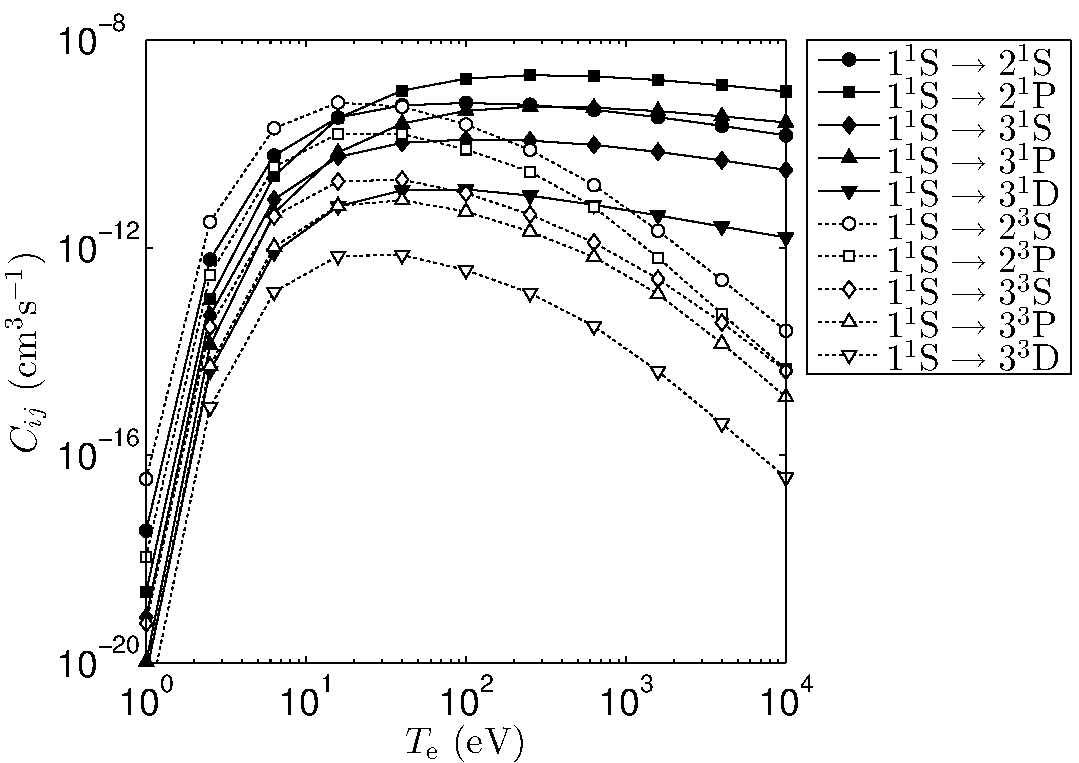
\includegraphics[height=0.35\textheight]{excRate-from-1.pdf}
  \caption{氦原子基态的电子碰撞激发速率系数,计算自 \onlinecite{Ralchenko2008603,NIFS:DATA:059} 的电子碰撞截面数据。}
  \label{fig:chap01:excRate:gs}
\end{figure}

氦原子的能级结构特点决定了其发射光谱适合用来进行托卡马克等离子体的诊断。

首先,氦原子能级结构拥有自旋单重态(singlet)和三重态(triplet)两套电子自旋系统。自旋三重态能级只能通过自旋变化过程激发产生,而自旋单重态能级主要通过自旋守恒过程从基态激发产生,不同自旋系统能级间的电子碰撞跃迁反应截面与相同自旋系统能级间电子碰撞跃迁的反应截面具有不同的随 $T_{\rm e}$ 的变化行为(图 \ref{fig:chap01:excRate:gs}--\ref{fig:chap01:excRate:metasinglet})。对于基态原子,当电子温度高于 $20\,{\rm eV}$ 时,自旋变化和自旋守恒过程的电子碰撞速率系数变化趋势开始有明显的差别(图 \ref{fig:chap01:excRate:gs}),自旋守恒激发过程的速率系数在 $T_{\rm e}$ 为几百电子伏时具有最高值,并且当 $T_{\rm e}$ 在 $50\,{\rm eV}$ 至 $1\,{\rm keV}$ 范围可以视为常数,而自旋变化过程的电子碰撞激发速率系数在 $T_{\rm e}\sim 20\,{\rm eV}$ 时达到最高值,随着 $T_{\rm e}$ 的升高大致按照 $T_{\rm e}^{-2}$ 的速率下降。氦原子亚稳态原子 $2^3{\rm S}$ 和 $2^1{\rm S}$ 的碰撞激发速率系数在图 \ref{fig:chap01:excRate:metatriplet} 和图 \ref{fig:chap01:excRate:metasinglet} 中画出。可见,亚稳态电子碰撞激发速率系数的最高值出现在比基态更低的 $T_{\rm e}$ 处。两亚稳态的自旋守恒激发速率系数分布更为平坦,而自旋变化过程的速率系数在 $T_{\rm e}<10\,{\rm eV}$ 时就开始下降。同时,图 \ref{fig:chap01:excRate:metatriplet} 中画出了 $2^3{\rm S}$ 至 $2^1{\rm S}$ 的电子碰撞跃迁速率系数,它大概是激发至主量子数 $n=3$ 自旋单重态能级速率系数的 $10$ 倍。所以,来自从不同自旋系统能级的谱线强度之比与 $T_{\rm e}$ 有较强的函数关系,而来自相同自旋系统能级的谱线强度比与 $N_{\rm e}$ 具有较强的函数关系,通过测量氦原子谱线辐射可以同时确定等离子体的 $T_{\rm e}$ 和 $N_{\rm e}$ 。

\begin{figure}
  \centering
  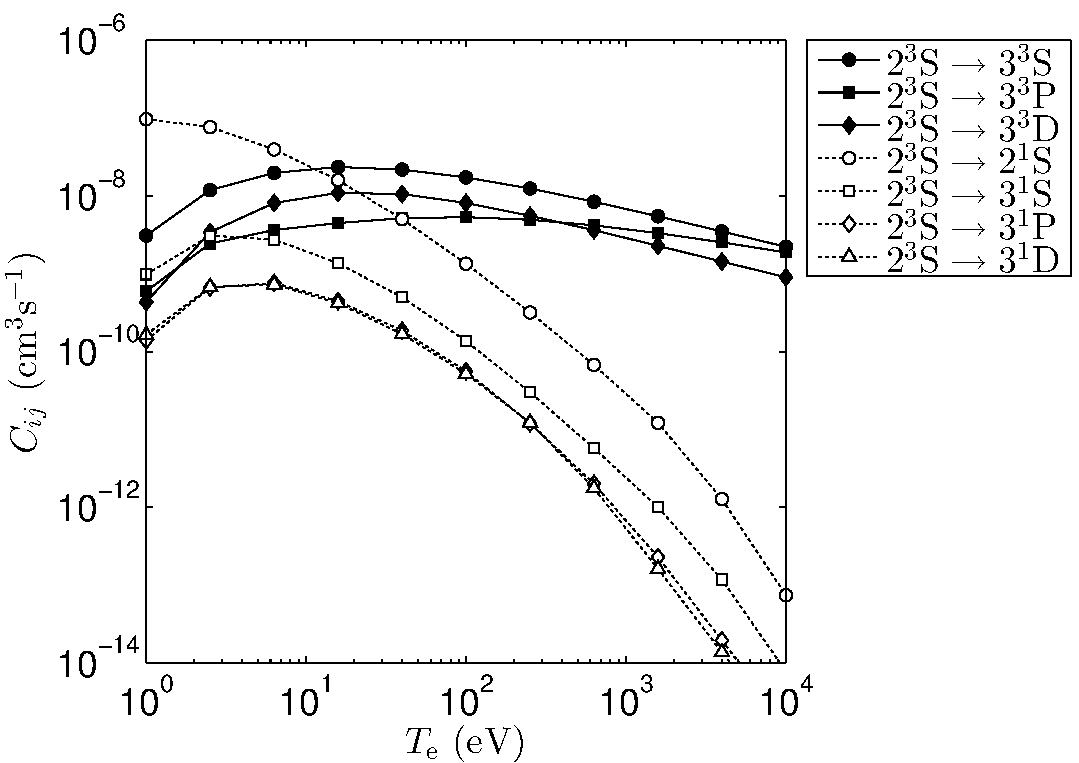
\includegraphics[height=0.35\textheight]{excRate-from-2.pdf}
  \caption{氦原子三重态亚稳态 $2^3{\rm S}$ 的电子碰撞激发速率系数,计算自 \onlinecite{Ralchenko2008603,NIFS:DATA:059} 的电子碰撞截面数据。}
  \label{fig:chap01:excRate:metatriplet}
\end{figure}

其次,在所有原子中,氦原子具有最高的基态电离能 $24.6\,{\rm eV}$。在氦原子束诊断托卡马克等离子体时,诊断束可以达到更深的位置,从而拓宽了诊断范围。

最后,氦为未来聚变等离子体中的固有元素,只需被动地测量氦原子的谱线辐射即可获得等离子体参数信息,不会给等离子体带来新的杂质粒子,即使现阶段大型托卡马克装置中利用氦束进行主动诊断,打入真空室的氦也不会对等离子体本身产生明显的影响\cite{Schmitz2008}。

因此,氦原子的发射光谱诊断(atomic emission spectroscopy)在高温聚变等离子体研究中得到了充分的重视,ITER 装置也已经考虑将氦原子的谱线诊断作为一种重要的诊断手段\cite{Mullane2002}。

\begin{figure}
  \centering
  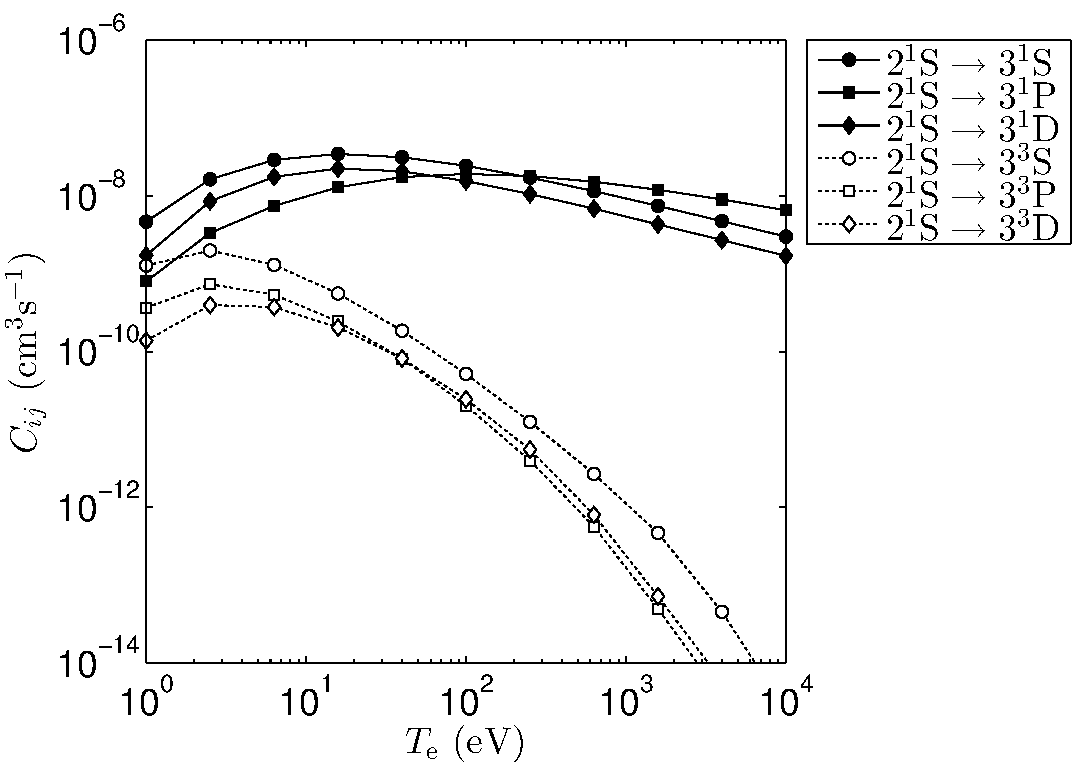
\includegraphics[height=0.35\textheight]{excRate-from-3.pdf}
  \caption{氦原子单重态亚稳态 $2^1{\rm S}$ 的电子碰撞激发速率系数,计算自 \onlinecite{Ralchenko2008603,NIFS:DATA:059} 的电子碰撞截面数据。}
  \label{fig:chap01:excRate:metasinglet}
\end{figure}


\subsection{氦原子发射光谱诊断的研究进展}
\label{sec:chap01:research-history}

最早提出使用自旋单重态和自旋三重态能级谱线辐射强度比方法测量等离子体电子温度的方法时
\cite{Sovie1964-He-coronal,Vries1966-He-coronal},是基于日冕模型(coronal model)的,后来研究中发现此方法只适用于电子密度很低的等离子体, 当 $N_{\rm e}$ 达到 $10^{11}\,{\rm cm}^{-3}$ 以上时,激发态的电子碰撞退激发过程对激发态数密度的影响加剧,此时应该使用碰撞辐射模型(collisional-radiative model)来计算激发态数密度分布\cite{Newe1966-He-CRRecommend}。

人们使用氦束发射光谱(beam emission spectroscopy)诊断等离子体参数是在 TEXTOR\cite{Schweer1992174} 上开始的。后来的类似诊断\cite{Davies1997-HeBES-JET,Field-HeBES-COMPASSD,Hidalgo-HeBES-TJII}
都使用了 TEXTOR 的碰撞辐射模型,该模型中考虑了包括基态在内的主量子数 $n\le 4$ 的共 19 个能级。当氦束为稳态束流时,束流中局域的氦原子激发态数密度保持稳定,只与本地的 $T_{\rm e}$ 和 $N_{\rm e}$ 相关,氦束在等离子体中直线传播,当氦原子被碰撞电离后,即沿磁力线运动而离开束流区域,所以氦离子的复合过程可以忽略,这样用于氦束发射光谱诊断的碰撞辐射模型被大大简化。

后来在 MST 上进行了高速氦束(fast helium beam)发射谱线的诊断研究\cite{Ahn2007-He-BES},并对例如杂质、磁场和离子碰撞等因素对谱线的影响进行了讨论,模型采用了 ADAS\cite{ADAS} 的代码和截面数据,包含了众多能级($n\le 110$),对主量子数能级 $n\le5$ 的能级根据 $nlSL$ 分别处理,将更高能级自旋相同的能级简并。最近 TEXTOR 对模型进行了进一步发展\cite{Schmitz2008},包括了较高的能级粒子,并对重粒子碰撞跃迁和电荷交换过程进行了考虑。而 MAP-II 偏滤器模拟装置\cite{Iida2010-HeBES-MAPII}的束发射光谱诊断工作中使用了 M. Goto 的模型\cite{Goto2003-HeCRM},并对辐射在等离子体中的捕获效应进行了讨论。

\begin{table}
\caption{氦束发射光谱诊断等离子体参数实验及使用的碰撞辐射模型}
{\small nlSL:能级以 nlSL 区分;nS:能级以自旋角动量区分;n:能级仅以主量子数区分;e-He:电子碰撞过程;rad:辐射过程;CX:电荷交换过程;ion-ion/dblion:离子碰撞电离与双电子电离;ion-exc/deexc:离子碰撞激发与退激发;D-tran:氘输运过程;rad-trap:辐射俘获效应。}
\label{tab:chap01:HeBES:CRM}
\begin{center}
\begin{tabular}{llllll}
\toprule[1.5pt]
       装置 & 区域 & 谱线能级 & 包含能级 & 包含过程 & 来源\\
\midrule[1pt]
    TEXTOR & 边界
            & $3^1{\rm D}$, $3^1{\rm S}$, $3^3{\rm S}$
            & $n\le4$
            & e-He, rad
            & \onlinecite{Schweer1992174} \\ \addlinespace[.5em]
    JET & 偏滤器
            & $3^1{\rm D}$, $3^1{\rm S}$, $3^3{\rm S}$
            & $n\le4$
            & e-He, rad
            & \onlinecite{Davies1997-HeBES-JET} \\ \addlinespace[.5em]
  COMPASS-D & 边界
            & $3^1{\rm D}$, $3^1{\rm S}$, $3^3{\rm S}$
            & $n\le4$
            & e-He, rad
            & \onlinecite{Field-HeBES-COMPASSD} \\ \addlinespace[.5em]
      TJ-II & 边界
            & $3^1{\rm D}$, $3^1{\rm S}$, $3^3{\rm S}$
            & $n\le4$
            & e-He, rad
            & \onlinecite{Hidalgo-HeBES-TJII} \\ \addlinespace[.5em]
    MST & 边界
            & $3^1{\rm D}$, $4^1{\rm D}$, $3^1{\rm P}$
            & \makecell[l]{nlSL: $n\le5$,\\
                nS: $6\le n\le 110$}
            & \makecell[l]{e-He, rad, CX\\
                ion-ion/dblion,\\ ion-exc/deexc}
            & \onlinecite{Ahn2007-He-BES} \\ \addlinespace[.5em]
    TEXTOR & 边界
            & $3^1{\rm D}$, $3^1{\rm S}$, $3^3{\rm S}$
            & \makecell[l]{nlSL: $n\le4$,\\
                nS: $5\le n\le 7$,\\
                n: $n=8, 9$, He$^+$}
            & \makecell[l]{e-He, rad, D-CX\\
                D-tran($\Delta n=0$)}
            & \onlinecite{Schmitz2008} \\ \addlinespace[.5em]
    MAP-II & \makecell[l]{偏滤器\\ 模拟装置}
            & \makecell[l]{$3^1{\rm D}$, $3^1{\rm P}$\\
                $4^3{\rm S}$, $3^3{\rm D}$, $3^3{\rm S}$}
            & 与 \onlinecite{Goto2003-HeCRM} 相同
            & \onlinecite{Goto2003-HeCRM}, rad-trap
            & \onlinecite{Iida2010-HeBES-MAPII} \\
\bottomrule[1.5pt]
\end{tabular}
\end{center}
\end{table}

表 \ref{tab:chap01:HeBES:CRM} 列出了用氦束发射光谱作为等离子体诊断手段的一些实验,这些实验主要集中在对边界和偏滤器等离子体的诊断,氦束发射光谱诊断法可以获得很高空间分辨率的 $T_{\rm e}$ 和 $N_{\rm e}$ 参数,对托卡马克等离子体的粒子输运、L--H 转换,MHD 约束行为的研究有很重要的作用。

在氦束发射光谱诊断的碰撞辐射模型处理上,氦原子被电离后便沿磁力线运动离开束流区域,在模型中则一般忽略氦离子对能级数密度的贡献。但是,在氦(或混入氦气)等离子体中,氦离子的影响则不再可以忽略,T. Fujimoto\cite{Fujimoto1979-HeCR} 建立了适用于低温氦气放电等离子体($N_{\rm e}=6.3\times10^{10}\,{\rm cm}^{-3}$, $T_{\rm e}=6\,{\rm eV}$)的碰撞辐射模型。在每种不同的等离子体条件下,添加不同的过程或外界条件的影响,T. Fujimoto 的模型在实验中得到了充分的应用和验证。同时,M. Goto 分别在 1997\cite{Goto1997-HeCRM-WT3} 和2003\cite{Goto2003-HeCRM} 年根据最新的碰撞截面数据对此模型进行了修订和更新。基于此模型在一些等离子体中的诊断应用总结于表 \ref{tab:chap01:FujimotoHeCRM:applications} 中。

\begin{table}
\caption{T. Fujimoto 的碰撞辐射模型在不同等离子体条件下的应用}
{\small wall: 器壁猝熄过程(quenching at wall);meta-meta:亚稳态原子非线性碰撞过程;$\nu$-abs/exc/ion:辐射吸收、激发与电离过程;hot-e:射频加热产生的热电子效应;res-scat:辐射的共振散射效应(resonance scattering of radiation);ionizing condition: 激发态粒子数密度独立于 ${\rm He}^+$ 密度。}
%\vspace{-1.5em}
\label{tab:chap01:FujimotoHeCRM:applications}
\begin{center}
\begin{tabular}{llll}
\toprule[1.5pt]
       装置 & 等离子体条件 & 添加过程或实验技术 & 来源\\
\midrule[1pt]
     - & 辉光放电
            & \makecell[l]{wall, meta-meta,\\ $\nu$-abs/exc/ion}
            & \onlinecite{Fujimoto1979-HeCR} \\ \addlinespace[.5em]
   NAGDIS-I & 氦等离子体
            & \makecell[l]{hot-e, res-scat}
            & \onlinecite{Sasaki1996-HeCRM-NAGDIS} \\ \addlinespace[.5em]
   JT-60U & \makecell[l]{偏滤器再循环氦}
            & \makecell[l]{ionizing condition}
            & \onlinecite{Hirotaka1999-HeCRM-JT60U} \\ \addlinespace[.5em]
   WT-3 & \makecell[l]{10\% 混氦}
            & \makecell[l]{$L-S$ 耦合}
            & \onlinecite{Goto1997-HeCRM-WT3} \\ \addlinespace[.5em]
   LHD & \makecell[l]{混氦}
            & \makecell[l]{$L-S$ 耦合}
            & \onlinecite{Goto2003-HeCRM} \\ \addlinespace[.5em]
  HYBTOK-II & \makecell[l]{氦等离子体}
            & \makecell[l]{CCD 相机 2 维测量}
            & \onlinecite{Ohno2010-HeCRM-2D-measure} \\
  H-1 & \makecell[l]{混氦}
            & \makecell[l]{计算机断层重建}
            & \onlinecite{MaShuiliang2012:Tomography} \\
\bottomrule[1.5pt]
\end{tabular}
\end{center}
\end{table}

从谱线强度比数据中分析出等离子体 $T_{\rm e}$ 和 $N_{\rm e}$ 的过程以碰撞辐射模型对等离子体谱线强度比与$T_{\rm e}$ 和 $N_{\rm e}$ 之间关系的计算为基础
\cite{Fujimoto1979-HeCR,Goto2003-HeCRM,boivin2001},碰撞辐射模型的建立包括选取模型包含的激发态能级,对能级之间电子碰撞反应过程的处理以及这些反应过程的速率系数(反应截面)的计算,在实际工作中,这些因素都会对模型的计算结果产生影响。早期的工作中\cite{Fujimoto1979-HeCR},人们期待在碰撞辐射模型中加入足够多的反应能级和碰撞辐射过程来满足计算结果的有效性,但由于包含的激发态能级不同,以及使用的速率系数精度较低\cite{Summers:IAEAdatarequirement},不同模型的计算结果差别较大
\cite{Boivin2007}。后来,M. Goto\cite{Goto2003-HeCRM}尝试更新模型的反应速率系数以获得精度更高的计算结果,同时 Y. Andrew 等人\cite{Andrew2000PPCFSensitivity}计算了模型中反应速率系数的不确定度对计算结果的影响,在 O. Schmitz 等人\cite{Schmitz2008}的工作中,将氦谱线比的诊断结果与其他诊断手段的结果进行对比来验证谱线比法诊断结果的有效性。

\begin{figure}%[H]
  \centering
  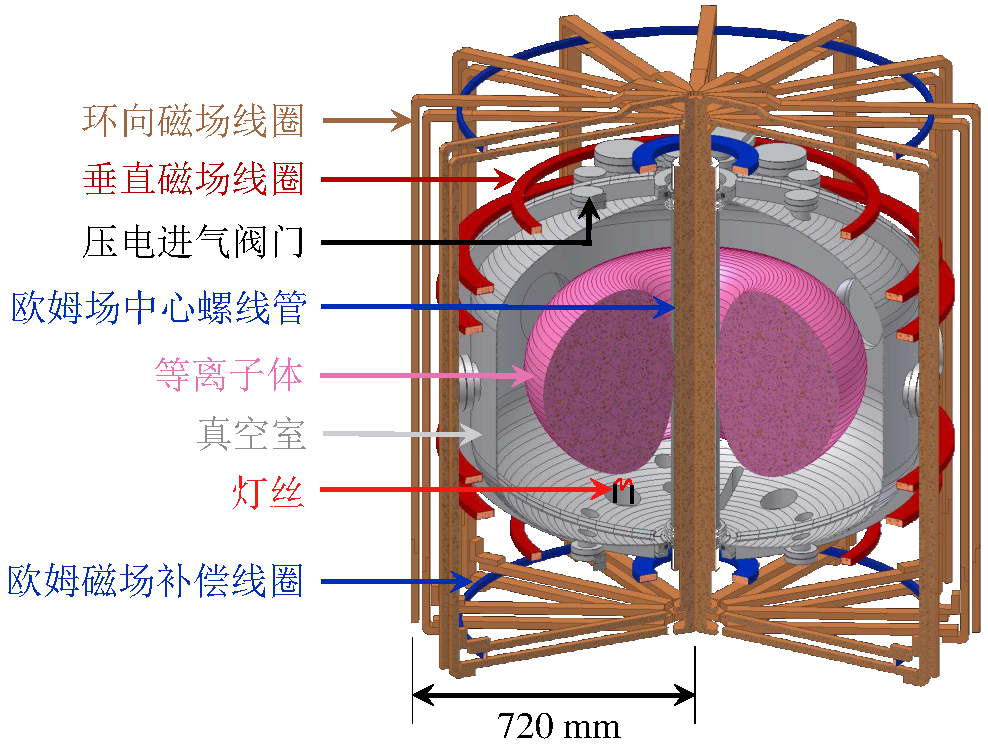
\includegraphics[width=0.8\textwidth]{SUNIST-Sketch-14_cropped.pdf}
  \caption{SUNIST 装置示意图,修改自\onlinecite{sunist:sketch:wiki}}
  \label{fig:chap01:sunist-sketch}
\end{figure}

%\subsection{国内研究现状}
\subsection{国内托卡马克等离子体的光谱诊断研究}

国内的托卡马克研究者也进行了大量的光谱诊断工作。在 CT-6B 装置中,李赞良等人\cite{LiZanliang:CT-6B:Te} 在 1989 年通过氧离子的真空紫外光谱测量了电流上升阶段的电子温度;后来赵庆勋等人\cite{ZhaoQingxun:CT-6B:Rotate}在 1997 年根据 OII $464.2\,{\rm nm}$、CIII $464.7\,{\rm nm}$ 和 ${\rm H}_\alpha$ 谱线的多普勒位移,测量了等离子体极向转动速度的径向分布。在 HT-7 装置上,刘建坤\cite{LiuJiankun2001:HT-7:PDA}等人使用光电二极管阵列,测量了 ${\rm H}_\alpha/{\rm D}_\alpha$ 的光谱,对粒子约束时间进行了系统研究;周倩等人\cite{ZhouQian2005:HT-7:carbon}在 2005 年通过对碳杂质的谱线辐射进行空间分辨测量,研究了碳杂质在径向的输运行为并在 2007 年完善了用于轻杂质粒子输运研究的光谱诊断系统;2010 年 HT-7 上用于电荷交换复合光谱诊断的诊断中心束束系统建成,实现了离子温度剖面分布测量\cite{ShiYuejiang2010:HT-7:CXRS};同时,陈开云等人\cite{ChenKaiyun2009:HT-7:SXTomography} 在 HT-7 上开展了基于断层扫描技术的软 X 射线诊断工作。在 J-TEXT 装置上通过测量软 X 射线辐射进行了反锯齿行为(inverse sawtooth activity)的研究\cite{FengXD2013:J-TEXT:softxray}。 崔正英等人\cite{CuiZhengying:2010:VUV}在 HL-2A 装置上建立了具有空间分辨诊断能力的真空紫外光谱测量系统,可以用于边界杂质和温度分布的测量。在 EAST 装置上,新建立了充气成像系统(gas puffing imaging),此系统可以有效的测量等离子体边界的湍流结构\cite{LiuSC:2012:EASTGPI},利用此系统成功研究了 L--H 转换的中间振荡过程(intermediate oscillatory phase)\cite{XuGS2014:EASTGPI:L-I-H}。

由此可见,虽然国内托卡马克光谱诊断研究众多,但基于碰撞辐射模型,通过测量原子谱线辐射强度比的方法诊断 $T_{\rm e}$ 和 $N_{\rm e}$ 参数的研究在国内尚未见报道。而低温等离子体研究领域,国内的研究者对此进行了大量有意义的研究工作\cite{ZhuXM2010:Review}。通过低温等离子体可见光谱辐射诊断的研究\cite{ZhuXM2009:Thesis} 发现,根据等离子体条件做必要的假设,通过在碰撞辐射模型中包含最主要的粒子和过程,可以对谱线比法诊断等离子体进行有效的指导。

\subsection{SUNIST 装置、等离子体参数范围与诊断需求}

\begin{figure}%[H]
  \centering
  \begin{overpic}[width=0.6\textwidth]{sunist_parram_vs_lineratio_range_2.pdf}
    \put(45,34){氦谱线比法}
	\put(51,45){SUNIST}
  \end{overpic}
  %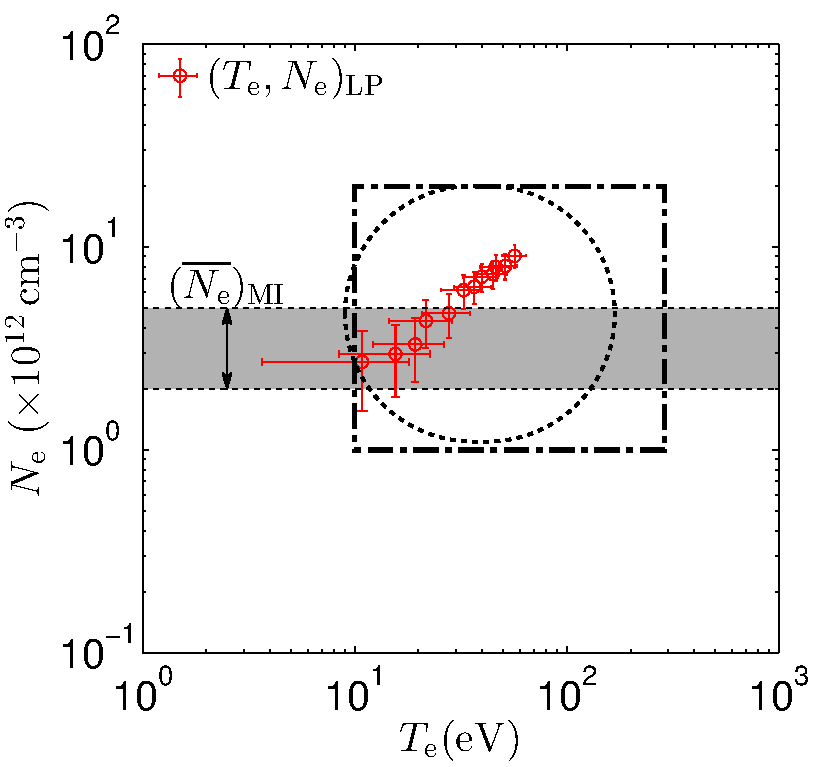
\includegraphics[width=0.6\textwidth]{sunist_parram_vs_lineratio_range_2.pdf}
  \caption{氦谱线比法诊断适用的电子参数范围与 SUNIST 等离子体参数范围估计。$(T_{\rm e},N_{\rm e})_{\rm LP}$ 表示静电探针测量的 SUNIST 边界等离子体参数\cite{WangWH2005:PPCF:Edge};$(\overline{N_{\rm e}})_{\rm MI}$ 表示微波干涉仪测量的电子密度范围值(第 \ref{sec:chap04:lineratio-ne-te} 节)。点划线表示氦原子谱线比法的适用范围;点线表示 SUNIST 等离子体电子参数估计范围。}
  \label{fig:chap01:te-ne-range}
\end{figure}

中国联合球形托卡马克(Sino-UNIted Spherical Tokamak,SUNIST)是我国第一台,也是唯一一台球形托卡马克装置\cite{Heyexi2002:SUNIST},图 \ref{fig:chap01:sunist-sketch} 所示为 SUNIST 装置示意图。

SUNIST 装置的主要参数为:大半径 $R_0=0.3\,{\rm m}$,小半径 $a=0.23\,{\rm m}$,欧姆放电时的等离子体电流 $I_{\rm p}\sim50\,{\rm kA}$,边界电子温度 $T_{\rm e}=20\,{\rm eV}\sim100\,{\rm eV}$ 和电子密度 $N_{\rm e}=1\times10^{12}\,{\rm cm}^{-3}\sim10\times10^{12}\,{\rm cm}^{-3}$\cite{WangWH2005:PPCF:Edge}(SUNIST 放电时的电子参数范围估计如图 \ref{fig:chap01:te-ne-range} 所示),真空室本底气压$p_{\rm gas,b}\sim5\times10^{-5}\,{\rm Pa}$,氦气放电充气气压范围 $p_{\rm gas}=2\times10^{-3}\,{\rm Pa}\sim5\times10^{-3}\,{\rm Pa}$。

%SUNIST 实验中,传统的等离子体电子参数诊断手段也面临着挑战,如静电探针会被高温等离子体烧蚀(图 \ref{fig:chap01:ProbeVapor}),这不但会缩短静电探针的使用寿命,而且会为诊断数据解析带来困难,烧蚀释放的重元素杂质粒子也会污染等离子体;同时,
SUNIST 做为小型球形托卡马克实验装置,研究人员匮乏,所以 SUNIST 装置亟需部署低成本、不干扰等离子体、少维护或免维护的可靠诊断手段。

%\begin{figure}%[H]
%  \centering
%  %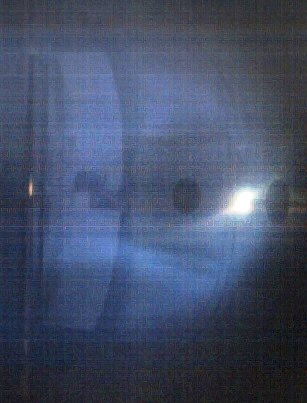
\includegraphics[height=0.3\textheight]{ProbeVapor121123020.jpg}
%  \begin{overpic}[scale=0.7]{ProbeVapor121123020-bw.jpg}
%    \put(1,22){\color{white}{\bf 中心柱}}
%    \put(2,29){\color{white}{$\uparrow$}}
%
%    \put(25,87){\color{white}{\bf 等离子体}}
%    \put(35,80){\color{white}{$\downarrow$}}
%
%    \put(50,59){\color{white}{\bf 静电探针}}
%    \put(67,53){\color{white}{$\downarrow$}}
%
%    \put(50,33){\color{white}{\bf 烧蚀亮点}}
%    \put(58,40){\color{white}{$\uparrow$}}
%  \end{overpic}
%  \caption{SUNIST放电时静电探针烧蚀情况(炮号:121123020)}
%  \label{fig:chap01:ProbeVapor}
%\end{figure}

\subsection{课题意义}
\label{sec:ketiyiyi}

利用等离子体的谱线辐射强度比进行诊断的方法具有不干扰等离子体,光谱测量设备简单且不受复杂电磁环境的影响以及仅需进行相对标定的优点。作为聚变产物,氦在未来聚变堆中是一种固有元素,所以利用氦原子谱线辐射强度比进行电子参数诊断不会为等离子体带入新的杂质,在高温聚变等离子体研究中得到了充分的重视。

然而,根据氦原子的谱线强度分析出 $T_{\rm e}$ 和 $N_{\rm e}$ 是以碰撞辐射模型对氦原子激发态数密度的计算为基础的。原子反应速率系数和碰撞辐射模型中包含的能级以及反应过程是影响碰撞辐射模型计算精度的主要因素。
%现阶段原子反应速率系数(或截面)数据主要有以下三种来源:实验测量
%\cite{Shah1988:ionizaiton-data-measure,Long1970:PhysRevA.1.260,Dixon1976}、
%理论计算\cite{CCCmethod,Sawey199381}与半经验公式拟合\cite{Fujimoto:IPPJ-AM-8},并且有人对此专门做过总结
%\cite{IAEA:Data:vol3,deHeer:INDC,Kato:NIFS:DATA:346}。然而这些数据来源的精度难以保证\cite{Ralchenko2008603},导致不同来源原子反应数据的碰撞辐射其计算结果也不尽相同\cite{Delabie2010:consistency}。%如第 \ref{sec:chap01:research-history} 节所述,
%为了得到更高精度的计算结果,人们往往在碰撞辐射模型中加入更多的能级粒子、反应过程以及可以对原子能级产生影响的因素。但因为使用的截面数据精度不一,导致碰撞辐射模型中包含更多的能级和反应过程时,并不能如预期那样获得更高精度的计算结果(第 \ref{sec:chap02:crm-problem} 节)。
%而且,
碰撞辐射模型中包含着众多的能级粒子和复杂的反应过程,且相互耦合,现并无有效的手段对碰撞截面数据不确定性到粒子数计算误差的传递进行有效计算的手段,也就无法对不同原子反应过程的数据提出具体的精度要求。
随着原子能级的升高,其原子数密度快速下降,在碰撞辐射模型中的重要性也随之下降。随之带来的问题是,在特定的等离子体参数条件下,碰撞辐射模型中包含至多高能级的激发态能级才能满足光谱诊断研究对精度的要求。
%或者由碰撞辐射模型中包含粒子数精简带来的误差会小于由原子反应速率系数精度的限制所带来的误差。

以上问题在托卡马克等离子体氦原子谱线比诊断的文献中鲜有报道。在低温等离子体研究领域,人们意识到这个问题\cite{ZhuXM2009:Thesis},并尝试在碰撞辐射模型中只包含与感兴趣能级粒子相关的主要过程,通过与实验的对比,来验证碰撞辐射模型的有效性。

在高温等离子体氦发射光谱诊断等离子体参数的实验中,适用的等离子体参数范围\cite{Schmitz2008} 为:$20\,{\rm eV}<T_{\rm e}<300\,{\rm eV}$ 与 $10^{12}\,{\rm cm}^{-3}<N_{\rm e}<2\times10^{12}\,{\rm cm}^{-3}$,这与 SUNIST 整个等离子体区域的参数范围一致(如图 \ref{fig:chap01:te-ne-range} 所示)。做为一台小型托卡马克装置,SUNIST 具有实验安排灵活的优势,适合进行诊断原理的验证性研究。
因此,我们在 SUNIST 中开展了氦原子光谱诊断研究。本文将根据 SUNIST 氦放电等离子体的特点建立碰撞辐射模型,研究影响模型计算结果的因素,包括速率系数不确定性和碰撞辐射模型中包含的能级粒子的影响等;验证利用氦原子谱线辐射强度比诊断 SUNIST 等离子体参数物理和技术上的可行性;并且在研究工作中为 SUNIST 完善运行设施,建立起光谱诊断系统,积累光谱诊断经验;同时,也希望为其他托卡马克装置采用此诊断提供参考。%奠定基础。

\section{本文研究思路、内容和结构}

\begin{figure}%[H]
  \centering
  
\includegraphics[width=0.8\textwidth]{research-progress.pdf}
  \caption{本论文研究过程图}
  \label{fig:chap01:research-progress}
\end{figure}

本文以氦放电等离子体的原子发射光谱诊断 $T_{\rm e}$ 和 $N_{\rm e}$ 为对象,完成了碰撞辐射模型的建立、实验系统建设、诊断方法的建立和验证等研究内容。图 \ref{fig:chap01:research-progress} 和图 \ref{fig:chap01:research-relationship} 分别显示的是本论文研究过程图和各部分研究内容之间的关系。

论文首先建立适用于 SUNIST 氦放电等离子体的碰撞辐射模型,然后根据模型对谱线比的预测与实验测量进行对比得到等离子体的 $T_{\rm e}$ 和 $N_{\rm e}$ 参数,最后验证该方法的有效性,并针对影响诊断结果的因素进行讨论。

在碰撞辐射模型方面,首先分析了 SUNIST 等离子体参数下的氦原子激发态数密度分布特点,选定模型粒子数密度方程中包含的激发态能级和反应过程,并选择合适的反应截面数据进行计算。该部分是光谱诊断的基础,为从谱线强度测量数据获得相应等离子体参数提供谱线强度比预测结果。

碰撞辐射模型在特定的等离子体参数空间提供了原子谱线强度比的预测结果,而通过实验数据获得对应参数则是一个反过程。为了获得实验数据,课题工作中建立了相应的光谱诊断设备,对单色仪各项参数进行了标定,并尽最大限度对光电倍增管的信号信号和干扰做了消除减弱。%首先需要对 SUNIST 的放电控制进行优化。同时需要建立起相应的实验测量设备,包括实验数据采集以及光谱诊断设备等。

对发射光谱法诊断手段的验证内容手段有:在诊断得到的等离子体参数下,模型计算的激发态能级数密度和实验测量对比对碰撞辐射模型的复核;影响模型对谱线比预测结果的因素\pozhehao 包括能级的选取、速率系数的不确定性等\pozhehao 的分析;以及光谱测量的弦积分特性带来的误差的分析等。

%论文各部分内容的关系如下(图 \ref{fig:chap01:research-relationship}):1)在给定的等离子体参数空间内,利用碰撞辐射模型给出的粒子数方程计算出谱线比方法感兴趣能级的数密度;2)将有效自发辐射跃迁速率系数与能级数密度相乘,得到氦原子谱线强度,进而计算出谱线强度比在等离子体参数空间的分布;3)把实验测得的谱线数据与光谱仪响应的标定结果相结合,得到实验测量的谱线强度比;4)将碰撞辐射模型计算与实验测量的谱线强度比进行对比,得到等离子体的具体 $T_{\rm e}$ 与 $N_{\rm e}$ 参数;5)在获得的 $T_{\rm e}$ 与 $N_{\rm e}$ 参数下,可以用碰撞辐射模型计算出所有实验中测量的谱线激发态能级的数密度,将其与实验测量数据计算得到的激发态数密度进行对比,复核碰撞辐射模型对等离子体中的碰撞与辐射过程描述。

通过氦原子谱线辐射诊断 $T_{\rm e}$ 和 $N_{\rm e}$ 的工作,本文建立了从模型建立到实验测量,再到数据分析以及对诊断结果进行评估的整体框架。

\begin{figure}%[H]
  \centering
  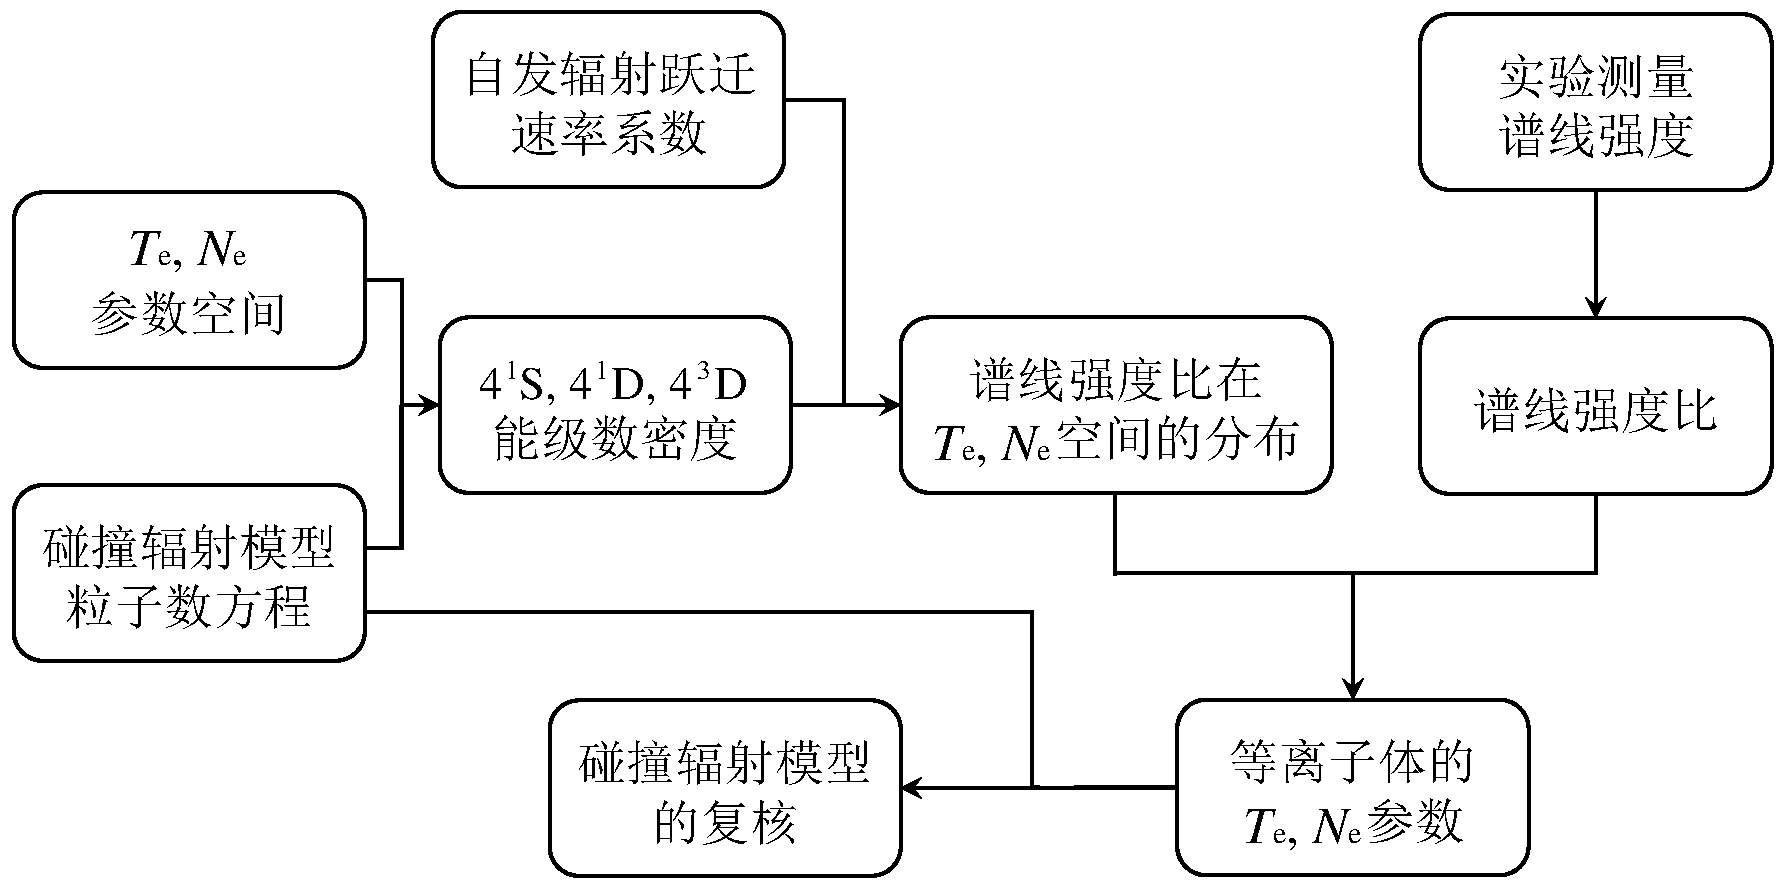
\includegraphics[width=\textwidth]{lineratio-method-rellevelabun.pdf}
  \caption{各部分研究内容的关系}
  \label{fig:chap01:research-relationship}
\end{figure}

本文结构如下:

第 \ref{chap:introduction} 章阐述了托卡马克高温聚变等离子体中光谱发射诊断研究的概况,介绍了本文研究的意义,给出了论文的主要研究内容和安排。

第 \ref{chap:crm-intro} 章从光子产生至被光谱系统检测测量所经历的物理过程出发,分析了影响谱线强度的因素:自发辐射跃迁几率、光子在等离子体内的传输以及自发辐射跃迁上能级激发态粒子数密度。给出了日冕、碰撞辐射模型和局域热平衡三种主要描述等离子体内粒子数密度分布的模型。介绍了高温聚变等离子体研究中使用的碰撞辐射模型的一般处理方法,并在最后指出现阶段氦原子谱线比诊断研究中使用的碰撞辐射模型所存在的一些问题,即反应速率系数不确定性至激发态数密度的传递估计手段不明确,以及模型中应包含的粒子和反应过程缺乏系统研究。

第 \ref{chap:crmodel} 章通过分析 SUNIST 氦放电等离子体内氦原子的特点(如原子能级数密度分布特点、等离子体的光学厚度、杂质影响和多种过程的时间常数等)建立了相应的碰撞辐射模型。通过选取使用前人整理的碰撞反应截面数据,求解了模型结果并与 FLYCHK 代码包的计算结果进行对比。最后,根据 SUNIST 氦放点等离子体的实验测量选取合适的谱线比,建立了氦原子谱线比诊断电子温度和密度的方法。

第 \ref{chap:measureing-system} 章介绍了 SUNIST 上的光谱诊断系统,包括光谱测量系统和测量路径安排,单色仪的谱线准确性、分辨率以及测量系统光谱响应的标定结果等。同时,介绍了降低信号噪声和消除基线干扰的手段,给出了 SUNIST 上基于重复放电的光谱测量手段以及氦原子谱线测量结果。相同的控制条件下 SUNIST 放电重复性的保证是测量的前提,本章也介绍了对提高放电重复性所做的研究,通过设计和安装 SUNIST 进气系统,改善了 SUNIST 放电的重复性。

第 \ref{chap:experiment} 章给出了 SUNIST 氦放电等离子体的光谱测量和等离子体电子温度与密度的诊断结果。通过其他未使用谱线对应激发态能级粒子数密度与碰撞辐射模型计算结果的对比,复核了本文建立的碰撞辐射模型。研究中还观察到弦积分光谱测量诊断的电子密度与微波干涉仪测量的弦平均电子密度的比值与电子参数剖面分布的峰化与否有直接关系、原子谱线强度与磁探针信号具有相同的涨落行为等结果,这为今后丰富和深入光谱诊断研究内容提供了参考和指引。

第 \ref{chap:summary} 章对本课题研究工作进行总结,指出工作的不足之处,并对未来的光谱诊断研究工作进行展望。


% \graphicspath{{figures/chap02/}}

%\chapter{等离子体原子发射谱线与碰撞辐射模型}
\chapter{原子谱线强度比诊断等离子体电子温度与密度概述}
\label{chap:crm-intro}

不同元素原子的能级结构是不相同的,具有不同的光谱辐射。通过对原子发射光谱的测量和分析,不仅可以定性地分析气体成分,还可以定量地分析各种元素的含量。根据不同原子受激发以及发射光谱的难易程度还可以进行等离子参数的诊断测量,例如电子温度 $T_{\rm e}$ 和电子密度 $N_{\rm e}$。

\section{原子谱线强度比诊断电子温度与密度}

原子受到激发后,由高能级 $j$ 跃迁到低能级 $i$ 时,将辐射出一定能量的光子,光子的波长 $\lambda_{ji}$ 由能级间的能量差 $\Delta E$ 决定:
\begin{equation}
  \lambda_{ji} = \frac{h{\rm c}}{\Delta E}
\end{equation}
式中,$h$ 为普朗克常数(Planck Constant),${\rm c}$ 为光速。其光子数辐射率可以写为\cite{Wiese1966:book}:
\begin{equation}
  %\label{}
  \epsilon_{ji}=\frac{1}{4\pi}N_{j}A_{ji}
\end{equation}
其中,$N_j$ 为跃迁上能级 $j$ 的粒子数密度,$A_{ji}$ 为自发辐射跃迁速率系数(爱因斯坦系数)。

假设均匀等离子体条件下,光谱测量系统获得的光子辐射计数率 $I_{\lambda_{ji}}$ 为:
\begin{equation}
  I_{\lambda_{ji}}=\epsilon_{ji}V\Omega T_{\lambda_{ji}}\eta_{\lambda_{ji}}
\end{equation}
其中,$V$ 为光谱仪可观测到的等离子体体积,$\Omega$ 为光谱接收设备所呈的立体角,$T_{\lambda_{ji}}$ 为等离子体的透射率,$\eta_{\lambda_{ji}}$ 为光学探测系统的量子效率。如果同时测量另外一条波长为 $\lambda_{qp}$ 的谱线,则两条谱线的强度比:
\begin{equation}
\label{eq:chap02:line-ratio}
  \frac{I_{\lambda_{ji}}}{I_{\lambda_{qp}}}=
  \frac{\epsilon_{ji}T_{\lambda_{ji}}\eta_{\lambda_{ji}}}{\epsilon_{qp}T_{\lambda_{qp}}\eta_{\lambda_{qp}}}
  =\frac{1}{F_R}\frac{T_{\lambda_{ji}}N_jA_{ji}}{T_{\lambda_{qp}}N_qA_{qp}}
\end{equation}
其中,$F_R$ 为与仪器响应相关的系数,实验中可以进行标定;自发辐射跃迁速率系数可以通过理论计算获得精确的数值,且一般不受等离子体参数的影响(第 \ref{sec:chap02:Aji} 节)。而由于跃迁上能级的粒子数密度 $N_{j}$ 与 $N_{q}$ 随电子温度与密度具有不同的变化趋势,这样通过建立反映原子反应过程的模型,事先计算出谱线比(式 \ref{eq:chap02:line-ratio})随等离子体电子温度与密度的变化趋势,在实验中测量出对应谱线的强度比,即可以根据模型计算结果反推出等离子体的电子温度和密度。

以 Z 箍缩氖等离子体中氖原子的 $K$ 壳层谱线辐射为例\cite{LiJing:WLXB},通过建立描述原子反应过程的碰撞辐射模型,计算出 ${\rm H}_\alpha$ 和 ${\rm I.C.}$ 谱线分别与 ${\rm He}_\alpha$ 谱线的强度比在电子温度--电子密度空间内的分布,其等高线如图 \ref{fig:chap02:lijing-a} 与 \ref{fig:chap02:lijing-b} 所示,其中谱线强度比 ${\rm H}_\alpha/{\rm He}_\alpha$ 主要与电子温度相关,谱线强度比 ${\rm I.C.}/{\rm He}_\alpha$ 主要与电子密度相关。如果在实验中同时测量该两谱线强度比值分别为 $0.53$ 与 $0.15$ 时,即可以同时确定等离子体的电子温度与密度参数,如图 \ref{fig:chap02:lijing-c} 所示。

\begin{figure}%[H]
  \centering
  \begin{subfigure}{0.45\textwidth}
  \begin{overpic}[width=\textwidth]{lijing-a.pdf}
    \put(15,63.5){\mbox{\colorbox{white}{\small\hspace{1em}}}}
    %\put(-2,30){\rotatebox{90}{\mbox{\colorbox{white}{\small\hspace{2em}激发截面 (${\rm m}^2$)\hspace{2em}}}}}
  \end{overpic}
  \caption{谱线强度比 ${\rm H}_\alpha/{\rm He}_\alpha$ 等高线}
  \label{fig:chap02:lijing-a}
  \end{subfigure}
  \hspace{0.03\textwidth}
  \begin{subfigure}{0.45\textwidth}
  \begin{overpic}[width=\textwidth]{lijing-b.pdf}
    \put(86,65){\mbox{\colorbox{white}{\hspace{0.5em}}}}
    %\put(-2,25){\rotatebox{90}{\mbox{\colorbox{white}{\small\hspace{2em}激发速率系数 (${\rm m}^3/{\rm s}$)\hspace{2em}}}}}
  \end{overpic}
  \caption{谱线强度比 ${\rm I.C.}/{\rm He}_\alpha$ 等高线}
  \label{fig:chap02:lijing-b}
  \end{subfigure}
  \\%\hspace{0.03\textwidth}
  \begin{subfigure}{0.45\textwidth}
  \begin{overpic}[width=\textwidth]{lijing-c.pdf}
    %\put(30,0){\mbox{\colorbox{white}{\small\hspace{2em}$T_{\rm e} (${\rm eV}$)$\hspace{2em}}}}
    %\put(-2,25){\rotatebox{90}{\mbox{\colorbox{white}{\small\hspace{2em}激发速率系数 (${\rm m}^3/{\rm s}$)\hspace{2em}}}}}
  \end{overpic}
  \caption{同时确定电子温度和密度的关系曲线}
  \label{fig:chap02:lijing-c}
  \end{subfigure}
  \caption{Z 箍缩氖等离子体中氖 $K$ 壳层的 ${\rm H}_\alpha$ 和 ${\rm I.C.}$ 与 ${\rm He}_\alpha$ 谱线的强度比的模型计算等高线(图 \ref{fig:chap02:lijing-a} 与 \ref{fig:chap02:lijing-b})与两谱线强度比分别为 $0.53$ 和 $0.15$ 时同时确定电子温度与密度的关系曲线(图 \ref{fig:chap02:lijing-c})。图片来自 \onlinecite{LiJing:WLXB}。}
  \label{fig:chap02:lijing}
\end{figure}

%\section{原子发射谱线}
\section{影响原子发射谱线强度的过程}

理论上要计算有多少光子辐射出等离子体区域,需要对以下三个过程进行分析:1)原子激发态自发辐射跃迁几率;2)特定的等离子体条件下原子激发态数密度;3)光子在等离子体中的传播。

\subsection{自发辐射跃迁几率}
\label{sec:chap02:Aji}

自发辐射跃迁几率可以通过原子物理相关理论计算获得,不同的等离子体环境(如温度、密度等)会对原子状态产生影响,但一般来讲等离子体环境对原子激发态自发辐射跃迁几率的影响微乎其微,可以忽略。$j\to i$ 自发辐射跃迁速率系数 $A_{ji}$ 可以由以下方程给出\cite{Kolb1964:A-formular}:
\begin{equation}
  A_{ji}=4.3\times10^7\frac{g_i}{g_j}f_{ij}\Delta E_{ji}^2\,{\rm s}^{-1}
\end{equation}
其中,$g_i$、$g_j$ 和 $\Delta E_{ji}$ 分别为 $i$、$j$ 能级的统计权重和两能级能量差,$f_{ij}$ 为 $i$ 到 $j$ 能级的吸收振子强度(absorption oscillator strength)\cite{Johnson1972:collisionalstrength}。另外,自发辐射跃迁系数也可以在数据库\cite{NISTdatabase}中直接查询获得。

\subsection{描述原子激发态数密度分布的模型}

%现阶段,爱因斯坦系数可以精确获得。而
式 (\ref{eq:chap02:line-ratio}) 中上能级的粒子数 $N_j$ 与 $N_q$ 与等离子体电子温度 $T_{\rm e}$ 和 $N_{\rm e}$ 相关。通过建立原子反应过程模型,事先计算等离子体辐射谱线上能级的粒子数密度与 $T_{\rm e}$ 和 $N_{\rm e}$ 的关系,则可通过测量谱线的强度比反推等离子体的电子温度和密度。

在特定的 $T_{\rm e}$ 和 $N_{\rm e}$ 参数下,通过对等离子体内影响特定原子激发态数密度的反应过程进行研究,以确定此激发态的数密度。这些原子反应过程一般为\cite{atomicprocesses,YuChangxuan:book}:

\begin{enumerate}
  \item 辐射跃迁
    \begin{itemize}
      \item 同步辐射跃迁(spontaneous radiative decay)
      \item 辐射复合(radiative recombination)
      \item 自发电离(autoionization)
      \item 双电子复合(dielectronic capture)
    \end{itemize}
  \item 自由电子碰撞
    \begin{itemize}
      \item 激发(excitation)
      \item 退激发(deexcitation)
      \item 电离(ionization)
      \item 复合(recombination)
    \end{itemize}
  \item 光致过程
    \begin{itemize}
      \item 光致激发(photoexcitation)
      \item 光致退激发(photodeexcitation)
      \item 光致电离(photoionization)
      \item 光致辐射复合(induced radiative recombination)
    \end{itemize}
  \item 重粒子碰撞
    \begin{itemize}
      \item 激发(excitation)
      \item 退激发(deexcitation)
      \item 电离(ionization)
      \item 电荷交换(charge exchange)
    \end{itemize}
\end{enumerate}

原则上,将这些过程的反应速率方程一一列出,并联立求解这些方程即可得到等离子体内各粒子的数密度。

但等离子体中包含了大量的粒子和数目巨大的相互碰撞反应过程,实际工作中不可能将所有反应过程进行描述并求解。实际的研究工作中,人们一般根据等离子体密度高低将等离子体分为三种模型进行描述:日冕模型、碰撞辐射模型和局域热平衡模型。图 \ref{fig:chap02:plasma_model_region} 所示为以拥有三个能级(基态和两个激发态能级)的原子为例,将三种模型的反应过程图像进行示意。

\begin{figure}%[H]
  \centering
  \begin{overpic}[width=0.9\textwidth]{plasma_model_region_used.pdf}
    \put(4,1){\mbox{\colorbox{white}{\hspace{2em}日冕图像\hspace{2em}}}}
    \put(36,1){\mbox{\colorbox{white}{\hspace{2em}碰撞辐射图像\hspace{2em}}}}
    \put(69,1){\mbox{\colorbox{white}{\hspace{2em}局域热平衡图像\hspace{2em}}}}
  \end{overpic}
  %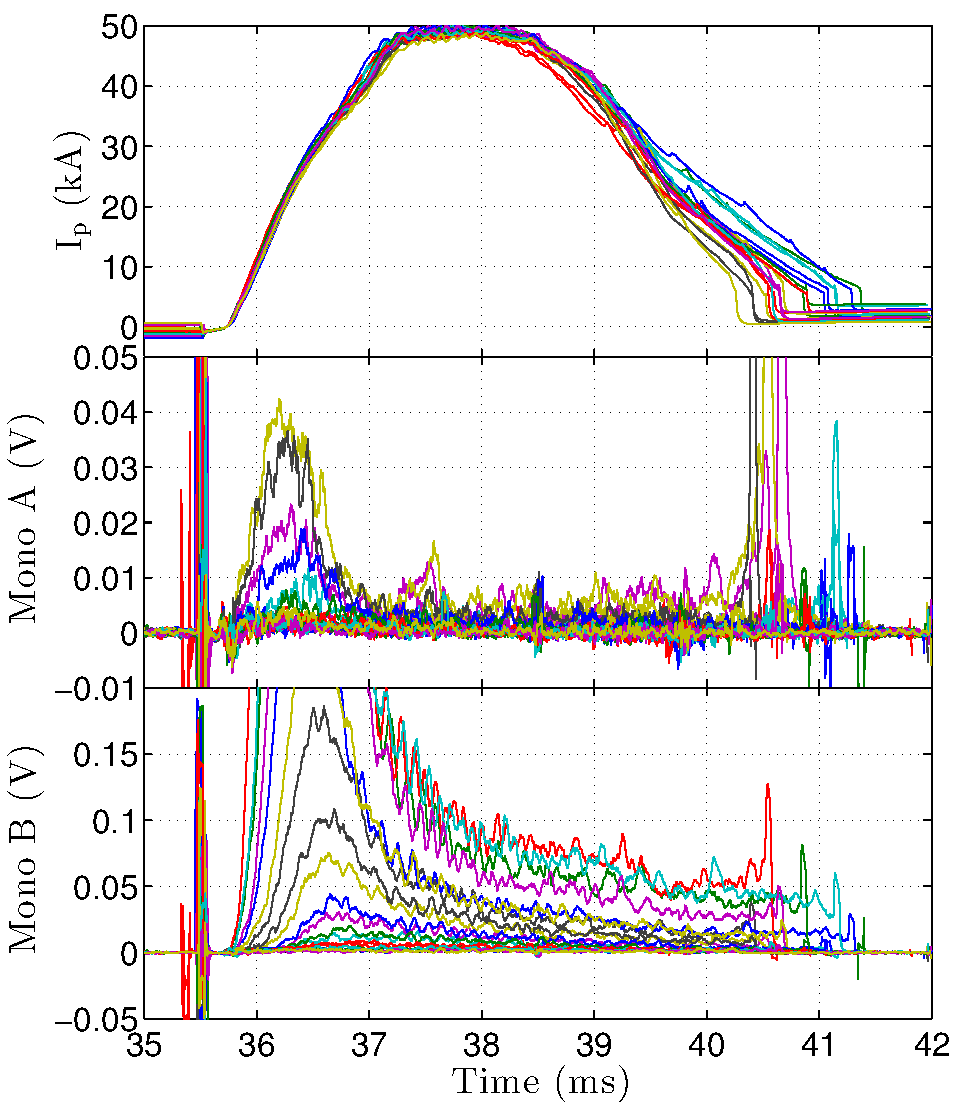
\includegraphics[width=0.7\textwidth]{AH72_BH32.pdf}
  \caption{具有三个能级(基态和两个激发态)原子的日冕图像、碰撞辐射图像和局域热平衡图像示意图。图片来自\onlinecite{Menhart2000:Thesis}。}
  \label{fig:chap02:plasma_model_region}
\end{figure}

\emph{日冕模型}\quad 在低密度等离子体($n<10^{11}\,{\rm cm}^{-3}$)中,等离子体内原子激发态的自发辐射跃迁几率远高于其碰撞损失过程(激发/退激发)的跃迁几率。所以,模型中仅考虑基态的碰撞激发、电离以及激发态的自发辐射跃迁过程。此时,激发态能级粒子的数密度要远低于基态能级的粒子数密度。

\emph{碰撞辐射模型}\quad 当等离子体密度较高时,碰撞过程反应速率增加。此时原子激发态数密度由碰撞和自发辐射过程的相互竞争决定。在碰撞辐射图像中,激发态原子的激发、退激发和电离过程等反应开始变得重要。托卡马克聚变等离子体的密度处在 $10^{11}\,{\rm cm}^{-3}\sim 10^{16}\,{\rm cm}^{-3}$ 区间,其原子反应过程应使用碰撞辐射模型描述。

\emph{局域热平衡模型}\quad 当等离子体密度高于 $10^{18}\,{\rm cm}^{-3}$ 时,碰撞反应过程的速率进一步加大,甚至超过自发辐射跃迁过程,此时激发态原子的自发辐射跃迁过程可以忽略。此时,原子激发态与基态之间处于局域热平衡状态。原子激发态之间和电离态之间的粒子数密度分布分别为麦克斯韦分布和萨哈分布,其分布函数可在 \onlinecite{YuChangxuan:book} 中找到。

\subsection{谱线辐射在等离子体内的传播}

激发态自发辐射跃迁产生的光子在等离子体的传播过程一般需要复杂的辐射输运方程进行描述\cite{Holstein1947:PhysRev.72.1212,Holstein1951:PhysRev.83.1159,Phelps1958:PhysRev.110.1362}。
实际计算中,人们一般采取简化的处理方法,如使用光学厚度和逃逸因子描述等离子体对光子辐射的吸收\cite{Johnson1972:collisionalstrength,boivin2001}。

其中,光学逃逸因子 $\Lambda$(optical escape factor)表示可以逃离等离子体区域的光子与总辐射光子的比例,逃逸因子接近或等于 $1$ 时,等离子体即为光性薄的。平均光学厚度 $\tau_0$(mean optical depth)为等离子体对光谱的指数吸收因子($I=I_0{\rm e}^{-\tau_0}$),当 $\tau_0\le0.01$ 时,对应的等离子体为光性薄的。

%要对逃逸因子和光学厚度进行计算,需要针对每条谱线辐射列出响应的辐射和吸收输运方程。
对于氦等离子体,如果谱线的多普勒展宽为主要展宽机制时\cite{Wiese1966:book},平均光学厚度和光学逃跑因子可以用下列公式计算\cite{Drawin1973:OEF,boivin2001}:
\begin{align}
  \tau_0&=\frac{n_ig_jA_{ji}\lambda_{ji,0}^3r}{8g_i\pi^{3/2}v_{\rm th}} \label{eq:chap02:mod}\\
  \Lambda&=1-\left(\frac{\tau_0}{\sqrt{2}}-\frac{\tau_0^2}{2!\sqrt{3}}+\frac{\tau_0^3}{3!\sqrt{4}}\cdots\frac{(-1)^{n+1}\tau_0^n}{n!\sqrt{n+1}}\right)
\end{align}
其中,$n_i$ 为跃迁低能级的粒子数密度,$g_j$ 和 $g_i$ 分别为跃迁对应高能级和低能级的统计权重,$\lambda_{ji,0}$ 为谱线的中心波长,$v_{\rm th}$ 为氦原子的热速度,$r$ 为等离子体特征尺度(半径)。另外,当谱线的主要展宽机制为非多普勒展宽时,J. He 等人\cite{HeJian2006:ef}计算了氦谱线辐射为洛仑兹(Lorentzian)和沃伊特(Voigt)线形时的逃逸因子。

\section{碰撞辐射模型}

%\subsection{原子反应速率方程}
托卡马克等离子体中的原子反应过程一般由碰撞辐射模型描述,对于等离子体内的某电离态离子的激发态能级粒子 $p$,其数密度 $N_p$ 随时间的变化由下面的速率方程决定:
\begin{equation}
\begin{aligned}
  \frac{{\rm d}N_p}{{\rm d}t}=
  &-\left\{\sum_{q\ne p}C_{pq}N_{\rm e}+\sum_{q<p}A_{pq}+S_{p\nu}N_{\rm e}+r_{p\mu}N_{\rm e}\right\}N_p\\
  &+\left\{\sum_{q\ne p}C_{qp}N_q+\sum_{q>p}A_{qp}N_q\right\}+\left\{S_{\mu p}N_{\mu}+r_{\nu p}N_\nu\right\}N_{\rm e}
\end{aligned}
\end{equation}
其中,$C$、$A$、$S$、$r$ 和 $N$ 分别表示电子碰撞激发或退激发速率系数、自发辐射跃迁几率、电子碰撞电离速率系数、电子碰撞复合速率系数和粒子数密度;下标中 $q$、$\mu$、$\nu$ 和 ${\rm e}$ 分别表示与 $p$ 能级具有相同电离态的 $q$ 激发态能级离子(或原子,下同)、低电离态离子、高电离态离子和电子。可见,对于 $p$ 能级粒子,其主要损失过程包括电子碰撞激发或退激发、电离和复合以及自发辐射跃迁过程;其产生过程也类似地由这些过程决定。

将等离子体内此电离态的基态和亚稳态粒子记为 $\rho$(在碰撞辐射模型中,亚稳态与其他普通激发态粒子的处理没有本质不同,其特性由原子反应过程的速率系数体现),其他激发态粒子记为 $i$,高电离态离子记为 $\nu$,低电离态粒子记为 $\mu$。对每个粒子的数密度 $N$ 列出其速率方程,即可得以下完备的粒子反应速率方程\cite{Summers2006}:
\begin{equation}
\label{eq:chap02:gcr}
\frac{{\rm d}}{{\rm d}t}
\begin{bmatrix}N_\mu\\ N_\rho\\ N_i\\ N_\nu\end{bmatrix}
=
\begin{bmatrix}
	\mathcal{C}_{\mu'} 	& N_{\rm e}\mathcal{R}_{\rho'\mu} & 0 & 0 \\
	N_{\rm e}\mathcal{S}_{\mu'\rho} & \mathcal{C}_{\rho'} & \mathcal{C}_{i'\rho} & N_e\mathcal{R}_{\nu'\rho} \\
	0 & \mathcal{C}_{\rho'i} & \mathcal{C}_{i'} & N_{\rm e}\mathcal{R}_{\nu'i} \\
	0 & N_{\rm e}\mathcal{S}_{\rho'\nu} & N_{\rm e}\mathcal{S}_{i'\nu} & \mathcal{C}_{\nu'}
\end{bmatrix}
\begin{bmatrix}
	N_{\mu'}\\ N_{\rho'}\\ N_{i'}\\ N_{\nu'}
\end{bmatrix}
\end{equation}
其中,方程右侧第一项碰撞辐射矩阵中,$\mathcal{S}$ 与 $\mathcal{R}$ 分别为离子的电离和复合速率系数向量。非对角元素 $\mathcal{C}$ 表示电子碰撞激发/退激发和自发辐射跃迁速率系数向量,以 $\mathcal{C}_{\rho'i}$ 为例:
\begin{equation}
  \mathcal{C}_{\rho'i}=\sum_{\rho'\ne i}C_{\rho'i}N_{\rm e}+\sum_{\rho'>i}A_{\rho'i}
\end{equation}
对角元素表示此粒子的总损失速率,以 $\mathcal{C}_{\rho'}$ 为例:
\begin{equation}
  \mathcal{C}_{\rho'}=-\left\{\left(\mathcal{R}_{\rho'\mu}+\mathcal{S}_{\rho'\nu}\right)N_{\rm e}+\mathcal{C}_{\rho'i}\right\}
\end{equation}
另外,粒子上标 $'$ 表示上一时刻的粒子数密度。

方程 (\ref{eq:chap02:gcr}) 描述了等离子体内各能级粒子(离子)的数密度随时间的变化。其中包含了两个假设:1)模型中只包含只有一个电子得失的电离和复合过程;2)电离和复合过程的产物粒子只处于基态或亚稳态。通过求解此方程可以获得随时间的演化情况,也可以计算系统达到稳态时的结果。对于达到平衡的磁约束聚变等离子体而言,等离子体中粒子碰撞和辐射跃迁过程的时间常数远小于等离子体的粒子约束时间,人们一般采用反应速率方程达到稳态时的计算结果。

%\section{前人在氦原子碰撞辐射模型研究中存在的问题}
\section{氦原子碰撞辐射模型在诊断应用中存在的问题}
\label{sec:chap02:crm-problem}
%\subsection{}

在利用氦原子谱线比诊断托卡马克等离子体 $T_{\rm e}$ 和 $N_{\rm e}$ 的研究中,为了得到更高精度的计算结果,人们不断尝试改进原子反应速率系数的精度,并增加在碰撞辐射模型中包含的能级粒子、反应过程以及可以对原子能级产生影响的因素。但因为使用的截面数据精度不一,导致碰撞辐射模型中包含更多的能级和反应过程时,并不能如预期那样获得更高精度的计算结果(图 \ref{fig:chap02:lineratio-compare-n3})。
%人们不断尝试改进原子反应速率系数的精度,并增加在碰撞辐射模型中包含的能级粒子,以期得到更高精度的激发态粒子数密度计算结果。

\begin{figure}%[H]
  \centering
  \begin{overpic}[width=\textwidth]{lineratio-compare-n3-black.pdf}
  \end{overpic}
  \caption{不同碰撞辐射模型计算的来自 $n=3$ 壳层的谱线比结果对比。(a):$T_{\rm e}=20\,{\rm eV}$ 时,$N_{\rm e}$ 敏感谱线比 $I_{667.8}/I_{728.1}$ 的对比;(b):$N_{\rm e}=1.0\times10^{12}\,{\rm cm}^{-3}$ 时,$T_{\rm e}$ 敏感谱线比 $I_{728.1}/I_{706.7}$ 的对比。模型和数据来源:Schweer1992:来自 \onlinecite{Schweer1992174} ($n\le4$);NIFS($n\le4$):来自 \onlinecite{Sasaki:NIFS:DATA:049};NIFS($n\le20$):来自 \onlinecite{Sasaki:NIFS:DATA:049};Kubo1999:来自 \onlinecite{Hirotaka1999-HeCRM-JT60U},使用 \onlinecite{Fujimoto1979-HeCR} 的模型;Ma2012:来自 \onlinecite{MaShuiliang2012:Tomography},使用 \onlinecite{Goto2003-HeCRM} 的模型;Burgos2012:来自 \onlinecite{burgos2012:PoP};CRM:本文碰撞辐射模型。}
  \label{fig:chap02:lineratio-compare-n3}
\end{figure}


1)原子反应速率系数不确定性

原子反应速率系数(或截面)数据主要有以下三种来源:实验测量
\cite{Shah1988:ionizaiton-data-measure,Long1970:PhysRevA.1.260,Dixon1976}、
理论计算\cite{CCCmethod,Sawey199381}与半经验公式拟合\cite{Fujimoto:IPPJ-AM-8},并且有人对此专门做过总结
\cite{IAEA:Data:vol3,deHeer:INDC,Kato:NIFS:DATA:346}。图 \ref{fig:chap02:xsec-compare} 所示为不同数据来源的电子碰撞激发和速率系数的对比。在碰撞辐射模型方面,人们也在一直将最新的速率系数总结结果应用在计算中,例如,M. Goto\cite{Goto2003-HeCRM} 将以前的碰撞辐射模型\cite{Fujimoto1979-HeCR} 使用的反应速率系数数据进行了更新。然而这些数据来源的精度难以保证\cite{Ralchenko2008603},导致不同来源原子反应数据的碰撞辐射其计算结果也不尽相同\cite{Delabie2010:consistency}。%如第 \ref{sec:chap01:research-history} 节所述,

碰撞辐射模型中包含着数目巨大的激发态能级和复杂的相关反应过程,且各粒子之间通过原子反应相互关联。目前并没有有效的手段可以对速率系数不确定性至激发态数密度计算误差之间的传递进行计算。Y. Andrew 等人\cite{Andrew2000PPCFSensitivity}提出了一种计算方法,在假设碰撞辐射模型中某一过程的速率系数具有不确定性时,对此速率系数进行干扰,并重新求解碰撞辐射模型,以获得该速率系数的不确定性对粒子数密度计算的影响。通过对所有的速率系数进行干扰并重新求解碰撞辐射模型,即可得到模型中各反应过程速率系数的影响。这种方法并不直观,速率系数不确定性至激发态数密度计算误差传递之间的物理意义不明确,且每次都要对碰撞辐射模型进行重新求解,也不能对速率系数精度提出具体的要求。

\begin{figure}%[H]
  \centering
  \begin{subfigure}{0.45\textwidth}
  \begin{overpic}[width=\textwidth]{meta-exc-xsec-compare.pdf}
    \put(30,0){\mbox{\colorbox{white}{\small\hspace{2em}$T_{\rm e} (${\rm eV}$)$\hspace{2em}}}}
    \put(-2,30){\rotatebox{90}{\mbox{\colorbox{white}{\small\hspace{2em}激发截面 (${\rm m}^2$)\hspace{2em}}}}}
  \end{overpic}
  \caption{电子碰撞激发 $2^3{\rm S}\to 3^3{\rm D}$ 的截面}
  \label{fig:chap02:xsec-compare-meta}
  \end{subfigure}
  \hspace{0.03\textwidth}
  \begin{subfigure}{0.45\textwidth}
  \begin{overpic}[width=\textwidth]{l-change-exc-rate-compare.pdf}
    \put(30,0){\mbox{\colorbox{white}{\small\hspace{2em}$T_{\rm e} (${\rm eV}$)$\hspace{2em}}}}
    \put(-2,25){\rotatebox{90}{\mbox{\colorbox{white}{\small\hspace{2em}激发速率系数 (${\rm m}^3/{\rm s}$)\hspace{2em}}}}}
  \end{overpic}
  \caption{电子碰撞激发 $3^3{\rm S}\to 3^3{\rm P}$ 的速率系数}
  \label{fig:chap02:xsec-compare-l-change}
  \end{subfigure}
  \caption{不同数据来源的电子碰撞激发和速率系数数据对比。图片来自
  \onlinecite{Goto1997-HeCRM-WT3},数据来源详见 \onlinecite{Goto1997-HeCRM-WT3} 的参考文献。}
  \label{fig:chap02:xsec-compare}
\end{figure}

2)模型中包含的激发态能级和反应过程

最早人们使用最高包含至 $n=4$ 壳层的碰撞辐射模型\cite{Brosda1993:Thesis,Schweer1992174},后来在模型中增加了 $5\le n\le9$ 的激发态和 ${\rm He}^+$\cite{Schmitz2008},随着模型的发展,包含了越来越多的能级\cite{Ahn2007-He-BES},甚至最高包含到了 $n=500$ 壳层的能级\cite{burgos2012:PoP}。然而,通过将这些模型谱线比的计算结果进行对比(图 \ref{fig:chap02:lineratio-compare-n3})发现,这些模型并没有因为包含了跟多的能级和反应过程而获得高精度的结果。

首先,对于很高激发态的能级,现阶段无法对其电子碰撞激发或电离的截面进行精确的理论计算,实验更是无法进行测量。模型中,只能通过经验上的定标关系来计算,然而这种定标关系的精度是很难保证的。其次,对于高激发态能级,其粒子数密度会急剧减少\cite{Fujimoto1979-HeCR,Griem1964-book},然而在模型中使用低精度的反应截面数据将其包含在计算中,这不但不会带来更高精度的计算结果,反而可能会带来更大的计算误差。目前,在使用相同的速率系数的前提下,在模型中包含不同的能级和反应过程对计算结果影响的研究还鲜有报道。其中,文献  \onlinecite{Sasaki:NIFS:DATA:049} 中给出了模型包含 $n\le4$ 和 $n\le20$ 时不同的计算结果,但没有详细分析模型中包含不同能级粒子时,计算结果将会呈现什么样的趋势。


\section{小结}

本章首先介绍了可同时诊断等离子体电子温度与密度的原子谱线辐射强度比法,然后从光子产生到被光谱测量设备探测接收所经历的物理过程出发,给出影响谱线强度的因素,包括:自发辐射跃迁几率、光子在等离子体内传播过程中的再吸收和激发态粒子数密度。其中,自发辐射跃迁几率系数可以获得高精度的数据,对于光性薄的等离子体,激发态粒子数密度与其电子密度和电子温度参数相关,通过建立描述等离子体内各粒子的原子反应速率方程,即可以求解出在不同的等离子体参数情况下的激发态粒子数密度。通过实验测量来自不同激发态的谱线,根据其谱线强度比,既可以反推出等离子体的电子温度和密度参数。

在实际研究中,人们根据等离子体密度的不同对等离子体内的反应过程进行不同的简化。对高温聚变等离子体,需要使用碰撞辐射模型以计入原子碰撞激发/退激发、电离/复合以及自发辐射跃迁等过程,以求解激发态粒子数密度。然而,原子反应过程速率系数(截面)数据的精度受到很大限制,以致人们在模型中包含越来越多的能级粒子和反应过程,却不能如预期的那样得到更高精度的结果。同时,由于碰撞辐射模型中包含了数目巨大的能级粒子和复杂的反应过程,目前并无有效手段对速率系数不确定性至能级粒子数密度计算误差的传递进行直接的有效计算。一般使用对速率系数进行干扰并再次求解模型的速率方程的方法,这种分析手段并不直观,也不易操作,对不确定性的传递也不能给出明确的物理意义。


%
%
% %%% 其它部分
% \backmatter
% % 插图索引
% \listoffigures
% % 表格索引
% \listoftables
% % 公式索引
% \listofequations
%
%
% % 参考文献
% \bibliographystyle{thubib}
% \bibliography{ref/refs}
%
%
% % 致谢
% %%% Local Variables:
%%% mode: latex
%%% TeX-master: "../main"
%%% End:

\begin{ack}
论文完成之际,回想读博历程。实验进展顺利时的欣喜若狂,理论计算无处入手时的绝望焦躁,熬到深夜周围的一片寂静……一幕幕浮上心头。学习工作中等到了很多人的帮助、支持与鼓励,感激之情无法用语言表达。这里我想用最笨拙的语言表达心中最真挚的感谢。

感谢导师高喆教授给予的教导、支持与帮助。课题研究工作中,高老师给我提出了很多建设性意见,为我明确研究方向提供了指引。并在论文形成撰写过程中付出了很多心血。

感谢蒲以康老师、王文浩老师、谭熠老师、解丽凤老师、彭晓炜老师给予的支持、教导、帮助与鼓励,从他们那里我学到了很多实验方法和技巧。

感谢王龙老师、杨宣宗老师和冯春华老师的关心、爱护与帮助。自本科大学生研究计划开始他们就一直在为我的工作提供帮助和建议,并给予了很多关系和爱护。

感谢张良、曾龙、赵爱慧、刘阳青、姜艳铮、柴忪以及其他师兄弟姐妹的帮助与在实验室的陪伴。

感谢工物系、西南物理研究院、等离子体物理研究所、工程物理研究院给予过我帮助的所有老师和同学。

感谢工作中在仪器制作、安装和调试中给过帮助的所有相关工程技术人员。

感谢我的父母的爱护与支持。尤其感谢张英女士,她的陪伴、支持与照顾是我支持下去的动力。

转眼间何也熙老师离开我们已经 6 年的时间,他为人和蔼,工作敬业,是我学习的榜样。再次对何老师表示深切怀念。

感谢我学习生活中出现过的所有人士。

本课题得到了国家自然科学基金(批准号:10990214、11175103、11261140327、11075092、11005067)和国际热核聚变实验堆(ITER)计划专项课题(批准号:2013GB112001)的资助,在此一并致谢。

感谢 \thuthesis,它的存在让我的论文写作轻松自在了许多,让我的论文格式规整漂亮了许多。
\end{ack}

%
% % 附录
% \begin{appendix}
% \input{data/appendix01}
% \end{appendix}
%
% % 个人简历
% \begin{resume}

  \resumeitem{个人简历}

  1984 年 2 月 10 日出生于河北省深州市。

  2002 年 9 月考入中国科学技术大学近代物理系,2006 年 7 月本科毕业并获得理学学士学位。

  2006 年 9 月免试进入清华大学工程物理系攻读核科学与技术博士学位至今。

  \resumeitem{发表的学术论文} % 发表的和录用的合在一起

  \begin{enumerate}[{[}1{]}]
  \item Huiqiao Xie, Zhe Gao, Yi Tan, et al. Electron temperature and density determination in helium plasmas of SUNIST using the optical emission spectrum line-ratio method. The Joint Meeting of 5th IAEA Technical Meeting on Spherical Tori \& 16th International Workshop on Spherical Torus (ISTW2011) \& 2011 US-Japan Workshop on ST Plasma, 2011: Toki.
  \bigskip
  %\vspace{-0.5em}
  \item Xie Huiqiao, Tan Yi, Ke Rui, et al. Analysis of the gas puffng performance for improving the repeatability of Ohmic discharges in the SUNIST spherical tokamak. In press. (已被 Plasma Science and Technology 录用. SCI 源刊.)
  \item 谢会乔, 谭熠, 刘阳青, 等. SUNIST 氦放电等离子体的碰撞辐射模型及其在谱线比法诊断的应用. (已被物理学报录用. SCI 源刊.)
  \end{enumerate}
%  \resumeitem{研究成果} % 有就写,没有就删除
%  \begin{enumerate}[{[}1{]}]
%  \item 任天令, 杨轶, 朱一平, 等. 硅基铁电微声学传感器畴极化区域控制和电极连接的
%    方法: 中国, CN1602118A. (中国专利公开号.)
%  \item Ren T L, Yang Y, Zhu Y P, et al. Piezoelectric micro acoustic sensor
%    based on ferroelectric materials: USA, No.11/215, 102. (美国发明专利申请号.)
%  \end{enumerate}
\end{resume}

%
% \end{document}
% \end{example}
%
% \subsection{选项}
% \label{sec:option}
% 本模板提供了一些选项以方便使用:
% \begin{description}
% \item[bachelor]
%   如果写本科论文将此选项打开。
%   \begin{example}
% \documentclass[bachelor]{thuthesis}
%   \end{example}
%
% \item[master]
%   如果写硕士论文将此选项打开。
%   \begin{example}
% \documentclass[master]{thuthesis}
%   \end{example}
%
% \item[doctor]
%   如果写博士论文将此选项打开。
%   \begin{example}
% \documentclass[doctor]{thuthesis}
%   \end{example}
%
% \item[postdoctor]
%   如果写博士博士后出站报告将此选项打开。
%   \begin{example}
% \documentclass[postdoctor]{thuthesis}
%   \end{example}
%
% \item[secret]
%   涉秘论文开关。配合另外两个命令 |\secretlevel| 和 |\secretyear| 分别用来指定保
%   密级别和时间。二者默认分别为\textbf{秘密}和当前年份。可以通过:
%   \cs{secretlevel}|{|绝密|}| 和 \cs{secretyear}|{|10|}| 年独立修改。
%   \begin{example}
% \documentclass[bachelor, secret]{thuthesis}
%   \end{example}
%
% \changes{v3.0}{2007/05/12}{不用专门为本科论文生成\textbf{提交}版本了。}
%
% \item[openany, openright]
%   正规出版物的章节出现在奇数页,也就是右手边的页面,这就是 \texttt{openright},
%   也是 \thuthesis 的默认选项。在这种情况下,如果前一章的最后一页也是奇数,那么
%   模板会自动生成一个纯粹的空白页,很多人不是很习惯这种方式,而且学校的格式似乎
%   更倾向于页面连续,那就是通常所说的 \texttt{openany}。{\fangsong 目前所有论文都是
%      openany。}这两个选项不用专门设置,\thuthesis{} 会根据当前论文类型自动选
%   择。
%
% \item[winfonts,adobefonts,nofonts]
%   这些选项用来指导 ctex 宏包/文档类设置选用的中文字体。
%   winfonts 指定使用中易的六款字体(XeTeX 下为四种)。adobefonts 指定使用 Adobe 的
%   四款免费中文字体,nofonts 不提供可用的中文字体,由用户自行设定。
%
% \item[arial]
%   使用真正的 arial 字体。此选项会装载 arial 字体宏包,如果此宏包不存在,就装
%   载Helvet。arialtoc 和 arialtitle 不受 arial 的影响。因为一般的 \TeX{} 发行都
%   没有 arial 字体,所以默认采用 Helvet,因为二者效果非常相似。如果你执着的要
%   用arial 字体,请参看:\href{http://www.mail-archive.com/ctan-ann@dante.de/msg00627.html}{Arial
%     字体}。
%
% \item[arialtoc]
%  目录项(章目录项除外)中的英文是否用 arial 字体。本选项和下一个 \textsl{arialtitle} 都不用用户
%  操心,模板都自动设置好了。
%
% \item[arialtitle]
%  章节标题中英文是否用 arial 字体(默认打开)。
% \end{description}
%
% \subsection{字体配置}
% \label{sec:font-config}
% 正确配置中文字体是使用模板的第一步。模板调用 ctex 宏包,提供如下字体使用方式:
% \begin{itemize}
%   \item 基于传统 CJK 包,使用 latex、pdflatex 编译;
%   \item 基于 xeCJK 包,使用 xelatex 编译。
% \end{itemize}
%
% 第一种方式的字体配置比较繁琐,建议使用 donated 制作的中文字体包(自
% 包含安装方法),请用户自行下载安装,此处不再赘述。本模板推荐使用第二
% 种方法,只要把所需字体放入系统字体文件夹(也可以指定自定义文件夹)即
% 可。用户可以使用 winfonts,adobefonts,nofonts 选项来选择可用的中文字库,
% 缺省情况下为 winfonts 有效,使用中易字体。注意当使用 xelatex 编译时,
% winfonts 只有中易的四款字体(宋体、黑体、楷书和仿宋)可用,而本科生需要用到幼圆,
% 另外 Linux 系统缺少上述字体,这些用户可以通过指定 nofonts 选项,利用 fontname.def
% 文件配置所需字体。使用中易六种字体的配置如下:
% \begin{example}
% \ProvidesFile{fontname.def}
% \setCJKmainfont[BoldFont={SimHei},ItalicFont={KaiTi}]{SimSun}
% \setCJKsansfont{SimHei}
% \setCJKmonofont{FangSong}
% \setCJKfamilyfont{zhsong}{SimSun}
% \setCJKfamilyfont{zhhei}{SimHei}
% \setCJKfamilyfont{zhkai}{KaiTi}
% \setCJKfamilyfont{zhfs}{FangSong}
% \setCJKfamilyfont{zhli}{LiSu}
% \setCJKfamilyfont{zhyou}{YouYuan}
% \newcommand*{\songti}{\CJKfamily{zhsong}} % 宋体
% \newcommand*{\heiti}{\CJKfamily{zhhei}}   % 黑体
% \newcommand*{\kaishu}{\CJKfamily{zhkai}}  % 楷书
% \newcommand*{\fangsong}{\CJKfamily{zhfs}} % 仿宋
% \newcommand*{\lishu}{\CJKfamily{zhli}}    % 隶书
% \newcommand*{\youyuan}{\CJKfamily{zhyou}} % 幼圆
% \end{example}
%
% 对 Windows XP 来说如下,KaiTi 需要替换为 KaiTi\_GB2312,
% FangSong 需要替换为 FangSong\_GB2312。
%
% 宏包中包含了 ``zhfonts.py'' 脚本,为 Linux 用户提供一种交互式的方式
% 从系统中文字体中选择合适的六种字体,最终生成对应的 ``fontname.def''
% 文件。要使用它,只需在命令行输入该脚本的完整路径即可。
%
% 最后,用户可以通过命令
% \begin{shell}
% $ fs-list :lang=zh > zhfonts.txt
% \end{shell}
% 得到系统中现有的中文字体列表,并相应替换上述配置。
%
% \subsection{命令}
% \label{sec:command}
% 模板中的命令分为两类:一是格式控制,二是内容替换。格式控制如字体、字号、字距和
% 行距。内容替换如姓名、院系、专业、致谢等等。其中内容替换命令居多,而且主要集中
% 在封面上,其中有以本科论文为最(比硕士和博士论文多了\textbf{综合论文训练任务书}一
% 页)。首先来看格式控制命令。
%
% \subsubsection{基本控制命令}
% \label{sec:basiccom}
%
% \myentry{字体}
% \DescribeMacro{\songti}
% \DescribeMacro{\fangsong}
% \DescribeMacro{\heiti}
% \DescribeMacro{\kaishu}
% \DescribeMacro{\lishu}
% \DescribeMacro{\youyuan}
% 等分别用来切换宋体、仿宋、黑体、楷体、隶书和幼圆字体。
%
% \begin{example}
% {\songti 乾:元,亨,利贞}
% {\fangsong 初九,潜龙勿用}
% {\heiti 九二,见龙在田,利见大人}
% {\kaishu 九三,君子终日乾乾,夕惕若,厉,无咎}
% {\lishu 九四,或跃在渊,无咎}
% {\heiti 九五,飞龙在天,利见大人}
% {\songti 上九,亢龙有悔}
% {\youyuan 用九,见群龙无首,吉}
% \end{example}
%
% \myentry{字号}
% \DescribeMacro{\chuhao}
% 等命令定义一组字体大小,分别为:
%
% \begin{center}
% \begin{tabular}{lllll}
% \hline
% |\chuhao|&|\xiaochu|&|\yihao|&|\xiaoyi| &\\
% |\erhao|&|\xiaoer|&|\sanhao|&|\xiaosan|&\\
% |\sihao|& |\banxiaosi|&|\xiaosi|&|\dawu|&|\wuhao|\\
% |\xiaowu|&|\liuhao|&|\xiaoliu|&|\qihao|& |\bahao|\\\hline
% \end{tabular}
% \end{center}
%
% 使用方法为:\cs{command}\oarg{num},其中 |command| 为字号命令,|num| 为行距。比
% 如 |\xiaosi[1.5]| 表示选择小四字体,行距 1.5 倍。写作指南要求表格中的字体
% 是 \cs{dawu},模板已经设置好了。
%
% \begin{example}
% {\erhao 二号 \sanhao 三号 \sihao 四号  \qihao 七号}
% \end{example}
%
% \myentry{密级}
% \DescribeMacro{\secretlevel}
% \DescribeMacro{\secretyear}
% 定义秘密级别和年限:
%   \begin{example}
% \secretyear{5}
% \secretlevel{内部}
%   \end{example}
%
% \myentry{引用方式}
% \DescribeMacro{\onlinecite}

% 学校要求的参考文献引用有两种模式:(1)上标模式。比如``同样的工作有很
% 多$^{[1,2]}$\ldots''。(2)正文模式。比如``文[3] 中详细说明了\ldots''。其中上标
% 模式使用远比正文模式频繁,所以为了符合使用习惯,上标模式仍然用常规
% 的 |\cite{key}|,而 |\onlinecite{key}| 则用来生成正文模式。
%
% 关于参考文献模板推荐使用 \BibTeX{},关于中文参考文献需要额外增加一个 Entry: lang,将其设置为 \texttt{zh}
% 用来指示此参考文献为中文,以便 thubib.bst 处理。如:
% \begin{example}
% @INPROCEEDINGS{cnproceed,
%   author    = {王重阳 and 黄药师 and 欧阳峰 and 洪七公 and 段皇帝},
%   title     = {武林高手从入门到精通},
%   booktitle = {第~$N$~次华山论剑},
%   year      = 2006,
%   address   = {西安, 中国},
%   month     = sep,
%   lang      = "zh",
% }
%
% @ARTICLE{cnarticle,
%   AUTHOR  = "贾宝玉 and 林黛玉 and 薛宝钗 and 贾探春",
%   TITLE   = "论刘姥姥食量大如牛之现实意义",
%   JOURNAL = "红楼梦杂谈",
%   PAGES   = "260--266",
%   VOLUME  = "224",
%   YEAR    = "1800",
%   LANG    = "zh",
% }
% \end{example}
%
% \myentry{书脊}
% \DescribeMacro{\shuji}
% 生成装订的书脊,为竖排格式,默认参数为论文中文题目。如果中文题目中没有英文字母,
% 那么直接调用此命令即可。否则,就要像例子里面那样做一些微调(参看模板自带
% 的 shuji.tex)。下面是一个列子:
% \begin{example}
% \documentclass[bachelor]{thuthesis}
% \begin{document}
% \ctitle{论文中文题目}
% \cauthor{中文姓名}
% % |\shuji| 命令需要上面两个变量
% \shuji
%
% % 如果你的中文标题中有英文,那可以指定:
% \shuji[清华大学~\hspace{0.2em}\raisebox{2pt}{\LaTeX}%
% \hspace{-0.25em} 论文模板 \hspace{0.1em}\raisebox{2pt}%
% {v\version}\hspace{-0.25em}样例]
% \end{document}
% \end{example}
%
% \myentry{破折号}
% \DescribeMacro{\pozhehao}
% 中文破折号在 CJK-\LaTeX\ 里没有很好的处理,我们平时输入的都是两个小短线,比如这
% 样,{\heiti 中国——中华人民共和国}。这不符合中文习惯。所以这里定义了一个命令生成更
% 好看的破折号,不过这似乎不是一个好的解决办法。有同学说不能用在 |\section| 等命
% 令中使用,简单的办法是可以提供一个不带破折号的段标题:\cs{section}\oarg{没有破
%   折号精简标题}\marg{带破折号的标题}。
%
%
% \subsubsection{封面命令}
% \label{sec:titlepage}
% 下面是内容替换命令,其中以 |c| 开头的命令跟中文相关,|e| 开头则为对应的英文。
% 这部分的命令数目比较多,但实际上都相当简单,套用即可。
%
% 大多数命令的使用方法都是: \cs{command}\marg{arg},例外者将具体指出。这些命令都
% 在示例文档的 data/cover.tex 中。
%
% \myentry{论文标题}
% \DescribeMacro{\ctitle}
% \DescribeMacro{\etitle}
% \begin{example}
% \ctitle{论文中文题目}
% \etitle{Thesis English Title}
% \end{example}
%
% \myentry{作者姓名}
% \DescribeMacro{\cauthor}
% \DescribeMacro{\eauthor}
% \begin{example}
% \cauthor{中文姓名}
% \eauthor{Your name in PinYin}
% \end{example}
%
% \myentry{申请学位名称}
% \DescribeMacro{\cdegree}
% \DescribeMacro{\edegree}
% \begin{example}
% \cdegree{您要申请什么学位}
% \edegree{degree in English}
% \end{example}
%
% \myentry{院系名称}
% \DescribeMacro{\cdepartment}
% \DescribeMacro{\edepartment}
%
% \cs{cdepartment} 可以加一个可选参数,如:\cs{cdepartmentl}\oarg{精简}\marg{详
%   细},主要针对本科生的\textbf{综合论文训练}部分,因为需要填写的空间有限,最好
% 给出一个详细和精简院系名称,如\textbf{计算机科学与技术}和\textbf{计算机}。
% \begin{example}
% \cdepartment[系名简称]{系名全称}
% \edepartment{Department}
% \end{example}
%
% \myentry{专业名称}
% \DescribeMacro{\cmajor}
% \DescribeMacro{\emajor}
% \begin{example}
% \cmajor{专业名称}
% \emajor{Major in English}
% \end{example}
%
% \DescribeMacro{\cfirstdiscipline}
% \DescribeMacro{\cseconddiscipline}
% \begin{example}
% \cfirstdiscipline{博士后一级学科}
% \cseconddiscipline{博士后二级学科}
% \end{example}
%
% \myentry{导师姓名}
% \DescribeMacro{\csupervisor}
% \DescribeMacro{\esupervisor}
% \begin{example}
% \csupervisor{导师~教授}
% \esupervisor{Supervisor}
% \end{example}
%
% \myentry{副导师姓名}
% \DescribeMacro{\cassosupervisor}
% \DescribeMacro{\eassosupervisor}
% 本科生的辅导教师,硕士的副指导教师。
% \begin{example}
% \cassosupervisor{副导师~副教授}
% \eassosupervisor{Small Boss}
% \end{example}
%
% \myentry{联合导师}
% \DescribeMacro{\ccosupervisor}
% \DescribeMacro{\ecosupervisor}
% 硕士生联合指导教师,博士生联合导师。
% \begin{example}
% \ccosupervisor{联合导师~教授}
% \ecosupervisor{Tiny Boss}
% \end{example}
%
% \myentry{论文成文日期}
% \DescribeMacro{\cdate}
% \DescribeMacro{\edate}
% \DescribeMacro{\postdoctordate}
% 默认为当前时间,也可以自己指定。
% \begin{example}
% \cdate{中文日期}
% \edate{English Date}
% \postdoctordate{2009年7月——2011年7月} % 博士后研究起止日期
% \end{example}
%
% \myentry{博士后封面其它参数}
% \DescribeMacro{\catalognumber}
% \DescribeMacro{\udc}
% \DescribeMacro{\id}
% \begin{example}
% \catalognumber{分类号}
% \udc{udc}
% \id{编号}
% \end{example}
%
% \myentry{摘要}
% \DescribeEnv{cabstract}
% \DescribeEnv{eabstract}
% \begin{example}
% \begin{cabstract}
%  摘要请写在这里...
% \end{cabstract}
% \begin{eabstract}
%  here comes English abstract...
% \end{eabstract}
% \end{example}
%
% \myentry{关键词}
% \DescribeMacro{\ckeywords}
% \DescribeMacro{\ekeywords}
% 关键词用英文逗号分割写入相应的命令中,模板会解析各关键词并生成符合不同论文格式
% 要求的关键词格式。
% \begin{example}
% \ckeywords{关键词 1, 关键词 2}
% \ekeywords{keyword 1, key word 2}
% \end{example}
%
% \subsubsection{其它部分}
% \label{sec:otherparts}
% 论文其它主要部分命令:
%
% \myentry{符号对照表}
% \DescribeEnv{denotation}
% 主要符号表环境。简单定义的一个 list,跟 description 非常类似,使用方法参见示例
% 文件。带一个可选参数,用来指定符号列的宽度(默认为 2.5cm)。
% \begin{example}
% \begin{denotation}
%   \item[E] 能量
%   \item[m] 质量
%   \item[c] 光速
% \end{denotation}
% \end{example}
%
% 如果你觉得符号列的宽度不满意,那可以这样来调整:
% \begin{example}
% \begin{denotation}[1.5cm] % 设置为 1.5cm
%   \item[E] 能量
%   \item[m] 质量
%   \item[c] 光速
% \end{denotation}
% \end{example}
%
% \myentry{索引}
% 插图、表格和公式三个索引命令分别如下,将其插入到期望的位置即可(带星号的命令表
% 示对应的索引表不会出现在目录中):
%
% \begin{center}
% \begin{tabular}{ll}
% \hline
%   {\heiti 命令} & {\heiti 说明} \\\hline
% \cs{listoffigures} & 插图索引\\
% \cs{listoffigures*} & \\\hline
% \cs{listoftables} & 表格索引\\
% \cs{listoftables*} & \\\hline
% \cs{listofequations} & 公式索引\\
% \cs{listofequations*} & \\\hline
% \end{tabular}
% \end{center}
%
% \LaTeX{} 默认支持插图和表格索引,是通过 \cs{caption} 命令完成的,因此它们必须出
% 现在浮动环境中,否则不被计数。
%
% 有的同学不想让某个表格或者图片出现在索引里面,那么请使用命令 \cs{caption*},这
% 个命令不会给表格编号,也就是出来的只有标题文字而没有``表~xx'',``图~xx'',否则
% 索引里面序号不连续就显得不伦不类,这也是 \LaTeX{} 里星号命令默认的规则。
%
% 有这种需求的多是本科同学的英文资料翻译部分,如果你觉得附录中英文原文中的表格和
% 图片显示成``表''和``图''很不协调的话,一个很好的办法还是用 \cs{caption*},参数
% 随便自己写,具体用法请参看示例文档。
%
% 如果你的确想让它编号,但又不想让它出现在索引中的话,那就自己改一改模板的代码吧,
% 我目前不打算给模板增加这种另类命令。
%
% 公式索引为本模板扩展,模板扩展了 \pkg{amsmath} 几个内部命令,使得公式编号样式和
% 自动索引功能非常方便。一般来说,你用到的所有数学环境编号都没问题了,这个可以参
% 看示例文档。如果你有个非常特殊的数学环境需要加入公式索引,那么请使
% 用 \cs{equcaption}\marg{编号}。此命令表示 equation caption,带一个参数,即显示
% 在索引中的编号。因为公式与图表不同,我们很少给一个公式附加一个标题,之所以起这
% 么个名字是因为图表就是通过 \cs{caption} 加入索引的,\cs{equcaption} 完全就是为
% 了生成公式列表,不产生什么标题。
%
% 使用方法如下。假如有一个非 equation 数学环境 mymath,只要在其中写一
% 句 \cs{equcaption} 就可以将它加入公式列表。
% \begin{example}
% \begin{mymath}
%   \label{eq:emc2}\equcaption{\ref{eq:emc2}}
%   E=mc^2
% \end{mymath}
% \end{example}
%
% 当然 mymath 正文中公式的编号需要你自己来做。
%
% 同图表一样,附录中的公式有时候也不希望它跟全文统一编号,而且不希望它出现在公式
% 索引中,目前的解决办法就是利用 \cs{tag*}\marg{公式编号} 来解决。用法很简单,此
% 处不再罗嗦,实例请参看示例文档附录 A 的前两个公式。
%
% \myentry{简历}
% \DescribeEnv{resume}\DescribeMacro{\resumeitem}
% 开启个人简历章节,包括发表文章列表等。其实就是一个 chapter。里面的每个子项目请用命令 |\resumeitem{sub title}|。
%
% 这里就不再列举例子了,请参看示例文档的 data/resume.tex。
%
% \myentry{附录}
% \DescribeEnv{appendix}
% 所有的附录都插到这里来。因为附录会更改默认的 chapter 属性,而后面的{\heiti 个人简
%   历}又需要恢复,所以实现为环境可以保证全局的属性不受影响。
% \begin{example}
% \begin{appendix}
%  \input{data/appendix01}
%  \input{data/appendix02}
% \end{appendix}
% \end{example}
%
% \myentry{致谢声明}
% \DescribeEnv{ack}
% 把致谢做成一个环境更好一些,直接往里面写感谢的话就可以啦!下面是数学系一位同
% 学致谢里的话,拿过来做个广告,多希望每个人都能写这么一句啊!
% \begin{example}
% \begin{ack}
%   ……
%   还要特别感谢计算机系薛瑞尼同学在论文格式和 \LaTeX{} 编译等方面给我的很多帮助!
% \end{ack}
% \end{example}
%
% \myentry{列表环境}
% \DescribeEnv{itemize}
% \DescribeEnv{enumerate}
% \DescribeEnv{description}
% 为了适合中文习惯,模板将这三个常用的列表环境用 \pkg{paralist} 对应的压缩环境替
% 换。一方面满足了多余空间的清楚,另一方面可以自己指定标签的样式和符号。细节请参
% 看 \pkg{paralist} 文档,此处不再赘述。
%
% \changes{v3.0}{2007/05/12}{没有了综合论文训练页面,很多本科论文专用命令就消失了。}
%
% \subsection{数学环境}
% \label{sec:math}
% \thuthesis{} 定义了常用的数学环境:
%
% \begin{center}
% \begin{tabular}{*{7}{l}}\hline
%   axiom & theorem & definition & proposition & lemma & conjecture &\\
%   公理 & 定理 & 定义 & 命题 & 引理 & 猜想 &\\\hline
%   proof & corollary & example & exercise & assumption & remark & problem \\
%   证明 & 推论 & 例子& 练习 & 假设 & 注释 & 问题\\\hline
% \end{tabular}
% \end{center}
%
% 比如:
% \begin{example}
% \begin{definition}
% 道千乘之国,敬事而信,节用而爱人,使民以时。
% \end{definition}
% \end{example}
% 产生(自动编号):\\[5pt]
% \fbox{{\heiti 定义~1.1~~~} {道千乘之国,敬事而信,节用而爱人,使民以时。}}
%
% 列举出来的数学环境毕竟是有限的,如果想用{\heiti 胡说}这样的数学环境,那么很容易定义:
% \begin{example}
% \newtheorem{nonsense}{胡说}[chapter]
% \end{example}
%
% 然后这样使用:
% \begin{example}
% \begin{nonsense}
% 契丹武士要来中原夺武林秘笈。\pozhehao 慕容博
% \end{nonsense}
% \end{example}
% 产生(自动编号):\\[5pt]
% \fbox{{\heiti 胡说~1.1~~~} {契丹武士要来中原夺武林秘笈。\kern0.3ex\rule[0.8ex]{2em}{0.1ex}\kern0.3ex 慕容博}}
%
% \subsection{自定义以及其它}
% \label{sec:othercmd}
% 模板的配置文件 thuthesis.cfg 中定义了很多固定词汇,一般无须修改。如果有特殊需求,
% 推荐在导言区使用 \cs{renewcommand}。当然,导言区里可以直接使用中文。
%
%
% \section{致谢}
% \label{sec:thanks}
% 感谢这些年来一直陪伴 \thuthesis{} 成长的新老同学,大家的需求是模板前
% 进的动力,大家的反馈是模板提高的机会。
% 
% 此版本加入了博士后出站报告的支持,本意为制作一个支持清华所有学位报告
% 的模板,孰料学校于近期对硕士、博士论文规范又有调整,未能及时更新,见
% 谅!
%
% 本人已于近期离开清华,虽不忍模板存此瑕疵,然精力有限,必不能如往日及
% 时升级,还望新的同学能参与或者接手,继续为大家服务。
% 
% \StopEventually{\PrintChanges\PrintIndex}
% \clearpage
%
% \section{实现细节}
%
% \subsection{基本信息}
%    \begin{macrocode}
%<cls>\NeedsTeXFormat{LaTeX2e}[1999/12/01]
%<cls>\ProvidesClass{thuthesis}
%<cfg>\ProvidesFile{thuthesis.cfg}
%<cls|cfg>[2012/07/28 4.8dev Tsinghua University Thesis Template]
%    \end{macrocode}
%
% \subsection{定义选项}
% \label{sec:defoption}
% TODO: 所有的选项用 \pkg{xkeyval} 来重构,现在的太罗唆了。
%
% 定义论文类型以及是否涉密
% \changes{v2.4}{2006/04/14}{添加模板名称命令。}
% \changes{v2.5}{2006/05/19}{增加本科论文的提交选项 submit。}
% \changes{v2.5.1}{2006/05/24}{如果没有设置格式选项,报错。}
% \changes{v2.5.1}{2006/05/26}{submit 只能由本科用。}
% \changes{v2.5.3}{2006/06/03}{submit 选项的一个笔误。}
% \changes{v3.0}{2007/05/12}{删除 submit 选项。}
% \changes{v4.6}{2011/04/26}{增加 postdoctor 选项。}
%    \begin{macrocode}
%<*cls>
\hyphenation{Thu-Thesis}
\def\thuthesis{\textsc{ThuThesis}}
\def\version{4.8dev}
\newif\ifthu@bachelor\thu@bachelorfalse
\newif\ifthu@master\thu@masterfalse
\newif\ifthu@doctor\thu@doctorfalse
\newif\ifthu@postdoctor\thu@postdoctorfalse
\newif\ifthu@secret\thu@secretfalse
\DeclareOption{bachelor}{\thu@bachelortrue}
\DeclareOption{master}{\thu@mastertrue}
\DeclareOption{doctor}{\thu@doctortrue}
\DeclareOption{postdoctor}{\thu@postdoctortrue}
\DeclareOption{secret}{\thu@secrettrue}
%    \end{macrocode}
%
% \changes{v2.5.1}{2006/05/24}{如果选项设置了 dvips,但是用 pdflatex 编译,报错。}
% \changes{v2.6}{2006/06/09}{增加 dvipdfm 选项。}
% \changes{v4.5}{2009/01/03}{增加 xetex, pdftex 选项。}
% \changes{v4.8dev}{2013/03/02}{内部调用 ctex 宏包,自动检测编译引擎}
%
% 如果需要使用 arial 字体,请打开 [arial] 选项
%    \begin{macrocode}
\newif\ifthu@arial
\DeclareOption{arial}{\thu@arialtrue}
%    \end{macrocode}
%
% 目录中英文是否用 arial
%    \begin{macrocode}
\newif\ifthu@arialtoc
\DeclareOption{arialtoc}{\thu@arialtoctrue}
%    \end{macrocode}
% 章节标题中的英文是否用 arial
%    \begin{macrocode}
\newif\ifthu@arialtitle
\DeclareOption{arialtitle}{\thu@arialtitletrue}
%    \end{macrocode}
%
% noraggedbottom 选项
% \changes{4.8dev}{2013/03/05}{增加 noraggedbottom 选项。}
%    \begin{macrocode}
\newif\ifthu@raggedbottom\thu@raggedbottomtrue
\DeclareOption{noraggedbottom}{\thu@raggedbottomfalse}
%    \end{macrocode}
%
% 将选项传递给 ctexbook 类
%    \begin{macrocode}
\DeclareOption*{\PassOptionsToClass{\CurrentOption}{ctexbook}}
%    \end{macrocode}
%
% \cs{ExecuteOptions} 的参数之间用逗号分割,不能有空格。开始不知道,折腾了老半
% 天。
% \changes{v2.5.1}{2006/05/24}{ft,研究生院目录要 times,而教务处要 arial。}
% \changes{v2.5.1}{2006/05/26}{本科 openright,研究生 openany。}
% \changes{v3.1}{2007/10/09}{本科的目录又不要 arial 字体了。}
% \changes{v4.8dev}{2013/03/10}{使用 ctexbook 类,优于调用 ctex 宏包。}
% \changes{v4.8dev}{2013/05/29}{添加 nocap 选项,恢复默认标题样式,模板会进一步定制。}
%    \begin{macrocode}
\ExecuteOptions{utf,arialtitle}
\ProcessOptions\relax
\LoadClass[cs4size,a4paper,openany,nocap,UTF8]{ctexbook}
%    \end{macrocode}
%
% 用户至少要提供一个选项:指定论文类型。
%    \begin{macrocode}
\ifthu@bachelor\relax\else
  \ifthu@master\relax\else
    \ifthu@doctor\relax\else
      \ifthu@postdoctor\relax\else
        \ClassError{thuthesis}%
                   {You have to specify one of thesis options: bachelor, master or doctor.}{}
      \fi
    \fi
  \fi
\fi
%    \end{macrocode}
%
% \subsection{装载宏包}
% \label{sec:loadpackage}
%
% 引用的宏包和相应的定义。
%    \begin{macrocode}
\RequirePackage{ifxetex}
\RequirePackage{ifthen,calc}
%    \end{macrocode}
%
% \AmSTeX{} 宏包,用来排出更加漂亮的公式。
% \changes{v4.8}{2013/03/02}{no need to load amssymb since we use txfonts.}
%    \begin{macrocode}
\RequirePackage{amsmath}
%    \end{macrocode}
%
% 用很爽的 \pkg{txfonts} 替换 \pkg{mathptmx} 宏包,同时用它自带的 typewriter 字
% 体替换 courier。必须出现在 \AmSTeX{} 之后。
% \changes{v3.1}{2007/06/16}{replace mathptmx with txfonts.}
%    \begin{macrocode}
\RequirePackage{txfonts}
%    \end{macrocode}
%
% 图形支持宏包。
%    \begin{macrocode}
\RequirePackage{graphicx}
%    \end{macrocode}
%
% 并排图形。\pkg{subfigure}、\pkg{subfig} 已经不再推荐,用新的 \pkg{subcaption}。
% 浮动图形和表格标题样式。\pkg{caption2} 已经不推荐使用,采用新的 \pkg{caption}。
%    \begin{macrocode}
\RequirePackage[labelformat=simple]{subcaption}
%    \end{macrocode}
%
% \changes{v4.8}{2013/03/02}{no need to load indentfirst directly since we use ctex.}
%
% 更好的列表环境。
% \changes{v2.6.2}{2006/06/18}{去掉 \pkg{paralist} 的 newitem 和 newenum 选项,因为默
% 认是打开的。}
% \changes{v2.6.4}{2006/10/23}{增加 \texttt{neverdecrease} 选项。}
%    \begin{macrocode}
\RequirePackage[neverdecrease]{paralist}
%    \end{macrocode}
%
% raggedbottom,禁止Latex自动调整多余的页面底部空白,并保持脚注仍然在底部。
%    \begin{macrocode}
\ifthu@raggedbottom
  \RequirePackage[bottom]{footmisc}
  \raggedbottom
\fi
%    \end{macrocode}
%
% 中文支持,我们使用 ctex 宏包。
% \changes{v4.5}{2008/01/03}{加入 XeTeX 支持,需要 \pkg{xeCJK}。}
% \changes{v4.8dev}{2013/03/09}{reset baselinestretch after ctex's change.}
% \changes{v4.8dev}{2013/05/28}{在 CJK 模式下用 \pkg{CJKspace} 保留中英文间空格。}
%    \begin{macrocode}
\ifthu@bachelor
  \RequirePackage{CJKfntef}
\fi
\renewcommand{\baselinestretch}{1.0}
\ifxetex
  \xeCJKsetup{AutoFakeBold=true,AutoFakeSlant=true}
  \punctstyle{quanjiao}
  % todo: minor fix of CJKnumb
  \def\CJK@null{\kern\CJKnullspace\Unicode{48}{7}\kern\CJKnullspace}
  \defaultfontfeatures{Mapping=tex-text} % use TeX --
%    \end{macrocode}
% 默认采用中易的四款 (宋,黑,楷,仿宋) 免费字体。本科生还需要隶书,需要手工
% 修改 fontname.def 文件。缺少中文字体的 Linux 用户可以通过 fontname.def 文件定义字体。
%    \begin{macrocode}
  \ifCTEX@nofonts
    % vim: set ft=tex:
% This file is modified from ctex's ctex-xecjk-winfonts.def.

\ProvidesFile{fontname.def}
\setCJKmainfont[BoldFont={SimHei},ItalicFont={KaiTi}]{SimSun}
\setCJKsansfont{SimHei}
\setCJKmonofont{FangSong}

\setCJKfamilyfont{zhsong}{SimSun}
\setCJKfamilyfont{zhhei}{SimHei}
\setCJKfamilyfont{zhkai}{KaiTi}
\setCJKfamilyfont{zhfs}{FangSong}
\setCJKfamilyfont{zhli}{LiSu}
\setCJKfamilyfont{zhyou}{YouYuan}

\newcommand*{\songti}{\CJKfamily{zhsong}}
\newcommand*{\heiti}{\CJKfamily{zhhei}}
\newcommand*{\kaishu}{\CJKfamily{zhkai}}
\newcommand*{\fangsong}{\CJKfamily{zhfs}}
\newcommand*{\lishu}{\CJKfamily{zhli}}
\newcommand*{\youyuan}{\CJKfamily{zhyou}}

  \fi

  \setmainfont{Times New Roman}
  \setsansfont{Arial}
  \setmonofont{Courier New}
\else
  \RequirePackage{CJKspace}
%    \end{macrocode}
% arial 字体需要单独安装,如果不使用 arial 字体,可以用 helvet 字体 |\textsf|
% 模拟,二者基本没有差别。
%    \begin{macrocode}
  \ifthu@arial
    \IfFileExists{arial.sty}%
                 {\RequirePackage{arial}}%
                 {\ClassWarning{thuthesis}{no arial.sty availiable!}}
  \fi
\fi
%    \end{macrocode}
%
% 定理类环境宏包,其中 \pkg{amsmath} 选项用来兼容 \AmSTeX{} 的宏包
%    \begin{macrocode}
\RequirePackage[amsmath,thmmarks,hyperref]{ntheorem}
%    \end{macrocode}
%
% 表格控制
% \changes{v2.6}{2006/06/09}{增加 \pkg{longtable}。}
%    \begin{macrocode}
\RequirePackage{array}
\RequirePackage{longtable}
%    \end{macrocode}
%
% 使用三线表:\cs{toprule},\cs{midrule},\cs{bottomrule}。
%    \begin{macrocode}
\RequirePackage{booktabs}
%    \end{macrocode}
%
% 参考文献引用宏包。
%    \begin{macrocode}
\RequirePackage[numbers,super,sort&compress]{natbib}
%    \end{macrocode}
%
% 生成有书签的 pdf 及其开关,请结合 gbk2uni 避免书签乱码。
% \changes{v2.6}{2006/06/09}{去除 hyperref 选项,等待全局传递。}
%    \begin{macrocode}
\RequirePackage{hyperref}
\ifxetex
  \hypersetup{%
    CJKbookmarks=true}
\else
  \hypersetup{%
    unicode=true,
    CJKbookmarks=false}
\fi
\hypersetup{%
  bookmarksnumbered=true,
  bookmarksopen=true,
  bookmarksopenlevel=1,
  breaklinks=true,
  colorlinks=false,
  plainpages=false,
  pdfpagelabels,
  pdfborder=0 0 0}
%    \end{macrocode}
%
% dvips 模式下网址断字有问题,请手工加载 breakurl 这个宏包解决之。
% \changes{v4.4}{2008/05/12}{修复网址断字。}
% \changes{v4.8}{2013/03/04}{dvips method is deprecated. We ask their users to load it manually.}
%
% 设置 url 样式,与上下文一致
%    \begin{macrocode}
\urlstyle{same}
%</cls>
%    \end{macrocode}
%
%
% \subsection{主文档格式}
% \label{sec:mainbody}
%
% \subsubsection{Three matters}
% 我们的单面和双面模式与常规的不太一样。
% \changes{v2.5.1}{2006/05/23}{本科正文之后页码即用罗马数字,研究生不变。}
% \changes{v2.5.3}{2006/06/03}{第一章永远右开。}
% \changes{v4.4}{2008/05/30}{本科正文后的页码延续前面的阿拉伯数字,不再用罗马数
% 字。}
% \changes{v4.4}{2008/05/30}{本科取消了所有页眉,毫无疑问,在以后的修订中还会加
% 上的,我们等着看。}
%    \begin{macrocode}
%<*cls>
\renewcommand\frontmatter{%
  \if@openright\cleardoublepage\else\clearpage\fi
  \@mainmatterfalse
  \pagenumbering{Roman}
  \pagestyle{thu@empty}}
\renewcommand\mainmatter{%
  \if@openright\cleardoublepage\else\clearpage\fi
  \@mainmattertrue
  \pagenumbering{arabic}
  \ifthu@bachelor\pagestyle{thu@plain}\else\pagestyle{thu@headings}\fi}
\renewcommand\backmatter{%
  \if@openright\cleardoublepage\else\clearpage\fi
  \@mainmattertrue}
%</cls>
%    \end{macrocode}
%
%
% \subsubsection{字体}
% \label{sec:font}
%
% 重定义字号命令
%
% Ref 1:
% \begin{verbatim}
% 参考科学出版社编写的《著译编辑手册》(1994年)
% 七号       5.25pt       1.845mm
% 六号       7.875pt      2.768mm
% 小五       9pt          3.163mm
% 五号      10.5pt        3.69mm
% 小四      12pt          4.2175mm
% 四号      13.75pt       4.83mm
% 三号      15.75pt       5.53mm
% 二号      21pt          7.38mm
% 一号      27.5pt        9.48mm
% 小初      36pt         12.65mm
% 初号      42pt         14.76mm
%
% 这里的 pt 对应的是 1/72.27 inch,也就是 TeX 中的标准 pt
% \end{verbatim}
%
% Ref 2:
% WORD 中的字号对应该关系如下:
% \begin{verbatim}
% 初号 = 42bp = 14.82mm = 42.1575pt
% 小初 = 36bp = 12.70mm = 36.135 pt
% 一号 = 26bp = 9.17mm = 26.0975pt
% 小一 = 24bp = 8.47mm = 24.09pt
% 二号 = 22bp = 7.76mm = 22.0825pt
% 小二 = 18bp = 6.35mm = 18.0675pt
% 三号 = 16bp = 5.64mm = 16.06pt
% 小三 = 15bp = 5.29mm = 15.05625pt
% 四号 = 14bp = 4.94mm = 14.0525pt
% 小四 = 12bp = 4.23mm = 12.045pt
% 五号 = 10.5bp = 3.70mm = 10.59375pt
% 小五 = 9bp = 3.18mm = 9.03375pt
% 六号 = 7.5bp = 2.56mm
% 小六 = 6.5bp = 2.29mm
% 七号 = 5.5bp = 1.94mm
% 八号 = 5bp = 1.76mm
%
% 1bp = 72.27/72 pt
% \end{verbatim}
%
% \begin{macro}{\thu@define@fontsize}
% \changes{v2.6.2}{2006/06/18}{引入此命令重新定义字号。}
% 根据习惯定义字号。用法:
%
% \cs{thu@define@fontsize}\marg{字号名称}\marg{磅数}
%
% 避免了字号选择和行距的紧耦合。所有字号定义时为单倍行距,并提供选项指定行距倍数。
%    \begin{macrocode}
%<*cls>
\newlength\thu@linespace
\newcommand{\thu@choosefont}[2]{%
   \setlength{\thu@linespace}{#2*\real{#1}}%
   \fontsize{#2}{\thu@linespace}\selectfont}
\def\thu@define@fontsize#1#2{%
  \expandafter\newcommand\csname #1\endcsname[1][\baselinestretch]{%
    \thu@choosefont{##1}{#2}}}
%    \end{macrocode}
% \end{macro}
% \begin{macro}{\chuhao}
% \begin{macro}{\xiaochu}
% \begin{macro}{\yihao}
% \begin{macro}{\xiaoyi}
% \begin{macro}{\erhao}
% \begin{macro}{\xiaoer}
% \begin{macro}{\sanhao}
% \begin{macro}{\xiaosan}
% \begin{macro}{\sihao}
% \begin{macro}{\banxiaosi}
% \begin{macro}{\xiaosi}
% \begin{macro}{\dawu}
% \begin{macro}{\wuhao}
% \begin{macro}{\xiaowu}
% \begin{macro}{\liuhao}
% \begin{macro}{\xiaoliu}
% \begin{macro}{\qihao}
% \begin{macro}{\bahao}
%    \begin{macrocode}
\thu@define@fontsize{chuhao}{42bp}
\thu@define@fontsize{xiaochu}{36bp}
\thu@define@fontsize{yihao}{26bp}
\thu@define@fontsize{xiaoyi}{24bp}
\thu@define@fontsize{erhao}{22bp}
\thu@define@fontsize{xiaoer}{18bp}
\thu@define@fontsize{sanhao}{16bp}
\thu@define@fontsize{xiaosan}{15bp}
\thu@define@fontsize{sihao}{14bp}
\thu@define@fontsize{banxiaosi}{13bp}
\thu@define@fontsize{xiaosi}{12bp}
\thu@define@fontsize{dawu}{11bp}
\thu@define@fontsize{wuhao}{10.5bp}
\thu@define@fontsize{xiaowu}{9bp}
\thu@define@fontsize{liuhao}{7.5bp}
\thu@define@fontsize{xiaoliu}{6.5bp}
\thu@define@fontsize{qihao}{5.5bp}
\thu@define@fontsize{bahao}{5bp}
%    \end{macrocode}
% \end{macro}
% \end{macro}
% \end{macro}
% \end{macro}
% \end{macro}
% \end{macro}
% \end{macro}
% \end{macro}
% \end{macro}
% \end{macro}
% \end{macro}
% \end{macro}
% \end{macro}
% \end{macro}
% \end{macro}
% \end{macro}
% \end{macro}
% \end{macro}
%
% 正文小四号 (12pt) 字,行距为固定值 20 磅。
%    \begin{macrocode}
\renewcommand\normalsize{%
  \@setfontsize\normalsize{12bp}{20bp}
  \abovedisplayskip=10bp \@plus 2bp \@minus 2bp
  \abovedisplayshortskip=10bp \@plus 2bp \@minus 2bp
  \belowdisplayskip=\abovedisplayskip
  \belowdisplayshortskip=\abovedisplayshortskip}
%</cls>
%    \end{macrocode}
%
%
% \subsubsection{页面设置}
% \label{sec:layout}
% 本来这部分应该是最容易设置的,但根据格式规定出来的结果跟学校的 WORD 样例相差很
% 大,所以只能微调。
% \changes{v2.4}{2006/04/14}{把页面尺寸写入 dvi,避免有的用户通
%   过 dvips 不指定页面类型而得到古怪的结果。}
% \changes{v4.5.2}{2010/09/19}{研究生页面边距由 3.2cm 改为 3cm。}
% \changes{v4.7}{2012/05/29}{修改本科生页脚间距与样例基本一致。}
%    \begin{macrocode}
%<*cls>
\AtBeginDvi{\special{papersize=\the\paperwidth,\the\paperheight}}
\AtBeginDvi{\special{!%
      \@percentchar\@percentchar BeginPaperSize: a4
      ^^Ja4^^J\@percentchar\@percentchar EndPaperSize}}
\setlength{\textwidth}{\paperwidth}
\setlength{\textheight}{\paperheight}
\setlength\marginparwidth{0cm}
\setlength\marginparsep{0cm}
\ifthu@bachelor
  \addtolength{\textwidth}{-6.4cm}
  \setlength{\topmargin}{2.8cm-1in}
  \setlength{\oddsidemargin}{3.2cm-1in}
  \setlength{\footskip}{1.78cm}
  \setlength{\headsep}{0.6cm}
  \addtolength{\textheight}{-7.8cm}
\else
  \addtolength{\textwidth}{-6cm}
  \setlength{\topmargin}{2.2cm-1in}
  \setlength{\oddsidemargin}{3cm-1in}
  \setlength{\footskip}{0.6cm}
  \setlength{\headsep}{0.2cm}
  \addtolength{\textheight}{-6cm}
\fi
\setlength{\evensidemargin}{\oddsidemargin}
\setlength{\headheight}{20pt}
\setlength{\topskip}{0pt}
\setlength{\skip\footins}{15pt}
%</cls>
%    \end{macrocode}
%
% \subsubsection{页眉页脚}
% \label{sec:headerfooter}
% 新的一章最好从奇数页开始 (openright),所以必须保证它前面那页如果没有内容也必须
% 没有页眉页脚。(code stolen from \pkg{fancyhdr})
%    \begin{macrocode}
%<*cls>
\let\thu@cleardoublepage\cleardoublepage
\newcommand{\thu@clearemptydoublepage}{%
  \clearpage{\pagestyle{empty}\thu@cleardoublepage}}
\let\cleardoublepage\thu@clearemptydoublepage
%    \end{macrocode}
%
% 定义页眉和页脚。chapter 自动调用 thispagestyle{thu@plain},所以要重新定义 thu@plain。
% \changes{v2.0}{2005/12/18}{以前的太乱了,重新整理过清晰多了。}
% \changes{v2.1}{2006/03/01}{彻底放弃 fancyhdr,定义自己的样式。}
% \changes{v2.5}{2006/05/13}{本科的奇偶页眉不同。}
% \changes{v2.5}{2006/05/20}{增加 empty 页面样式。}
% \changes{v4.7}{2012/05/29}{本科页码用小五号字。}
% \begin{macro}{\ps@thu@empty}
% \begin{macro}{\ps@thu@plain}
% \begin{macro}{\ps@thu@headings}
% 定义三种页眉页脚格式:
% \begin{itemize}
% \item \texttt{thu@empty}:页眉页脚都没有
% \item \texttt{thu@plain}:只显示页脚的页码
% \item \texttt{thu@headings}:页眉页脚同时显示
% \end{itemize}
%    \begin{macrocode}
\def\ps@thu@empty{%
  \let\@oddhead\@empty%
  \let\@evenhead\@empty%
  \let\@oddfoot\@empty%
  \let\@evenfoot\@empty}
\def\ps@thu@plain{%
  \let\@oddhead\@empty%
  \let\@evenhead\@empty%
  \def\@oddfoot{\hfil\xiaowu\thepage\hfil}%
  \let\@evenfoot=\@oddfoot}
\def\ps@thu@headings{%
  \def\@oddhead{\vbox to\headheight{%
    \hb@xt@\textwidth{\hfill\wuhao\songti\leftmark\ifthu@bachelor\relax\else\hfill\fi}%
      \vskip2pt\hbox{\vrule width\textwidth height0.4pt depth0pt}}}
  \def\@evenhead{\vbox to\headheight{%
      \hb@xt@\textwidth{\wuhao\songti%
      \ifthu@bachelor\thu@schoolname\thu@bachelor@subtitle%
       \else\hfill\leftmark\fi\hfill}%
      \vskip2pt\hbox{\vrule width\textwidth height0.4pt depth0pt}}}
  \def\@oddfoot{\hfil\wuhao\thepage\hfil}
  \let\@evenfoot=\@oddfoot}
%    \end{macrocode}
% \end{macro}
% \end{macro}
% \end{macro}
%
% 其实可以直接写到 \cs{chapter} 的定义里面。
%    \begin{macrocode}
\renewcommand{\chaptermark}[1]{\@mkboth{\@chapapp\  ~~#1}{}}
%</cls>
%    \end{macrocode}
%
%
% \subsubsection{段落}
% \label{sec:paragraph}
%
% 段落之间的竖直距离
%    \begin{macrocode}
%<*cls>
\setlength{\parskip}{0pt \@plus2pt \@minus0pt}
%    \end{macrocode}
%
% 调整默认列表环境间的距离,以符合中文习惯。
% \changes{v2.5.2}{2006/06/01}{更改默认列表距离。}
% \begin{macro}{thu@item@space}
%    \begin{macrocode}
\def\thu@item@space{%
  \let\itemize\compactitem
  \let\enditemize\endcompactitem
  \let\enumerate\compactenum
  \let\endenumerate\endcompactenum
  \let\description\compactdesc
  \let\enddescription\endcompactdesc}
%</cls>
%    \end{macrocode}
% \end{macro}
%
%
% \subsubsection{脚注}
% \label{sec:footnote}
% \begin{macro}{\MakePerPage}
%   从 perpage.sty 中抽取的代码,使 footnote 按页编号。不再用臃肿的 footmisc。
%    \begin{macrocode}
%<*cls>
\newcommand*\MakePerPage[2][\@ne]{%
  \expandafter\def\csname c@pchk@#2\endcsname{\c@pchk@{#2}{#1}}%
  \newcounter{pcabs@#2}%
  \@addtoreset{pchk@#2}{#2}}
\def\new@pagectr#1{\@newl@bel{pchk@#1}}
\def\c@pchk@#1#2{\z@=\z@
  \begingroup
  \expandafter\let\expandafter\next\csname pchk@#1@\arabic{pcabs@#1}\endcsname
  \addtocounter{pcabs@#1}\@ne
  \expandafter\ifx\csname pchk@#1@\arabic{pcabs@#1}\endcsname\next
  \else \setcounter{#1}{#2}\fi
  \protected@edef\next{%
    \string\new@pagectr{#1}{\arabic{pcabs@#1}}{\noexpand\thepage}}%
  \protected@write\@auxout{}{\next}%
  \endgroup\global\z@}
\MakePerPage{footnote}
%    \end{macrocode}
% \end{macro}
%
% 脚注字体:宋体小五,单倍行距。悬挂缩进 1.5 字符。标号在正文中是上标,在脚注中为
% 正体。默认情况下 \cs{@makefnmark} 显示为上标,同时为脚标和正文所用,所以如果要区
% 分,必须分别定义脚注的标号和正文的标号。
% \changes{v2.1}{2006/03/01}{让脚注它悬挂起来,而且中文中用上标,脚注中用正体。}
% \changes{v2.5}{2006/05/13}{修正 minipage 中的脚注。}
% \changes{v2.5.1}{2006/05/21}{脚注编号使用 \cs{textcircled} 命令,每页允许至多 99 个
% 脚注条目。}
% \begin{macro}{\thu@textcircled}
% 生成带圈的脚注数字。最多处理到 99,当然这个很容易扩展了。
%    \begin{macrocode}
\def\thu@textcircled#1{%
  \ifnum \value{#1} <10 \textcircled{\xiaoliu\arabic{#1}}
  \else\ifnum \value{#1} <100 \textcircled{\qihao\arabic{#1}}\fi
  \fi}
%    \end{macrocode}
% \end{macro}
% \changes{v2.6}{2006/06/09}{脚注改成 1.5 倍行距,漂亮。}
%    \begin{macrocode}
\renewcommand{\thefootnote}{\thu@textcircled{footnote}}
\renewcommand{\thempfootnote}{\thu@textcircled{mpfootnote}}
\def\footnoterule{\vskip-3\p@\hrule\@width0.3\textwidth\@height0.4\p@\vskip2.6\p@}
\let\thu@footnotesize\footnotesize
\renewcommand\footnotesize{\thu@footnotesize\xiaowu[1.5]}
\def\@makefnmark{\textsuperscript{\hbox{\normalfont\@thefnmark}}}
\long\def\@makefntext#1{
  \bgroup
    \newbox\thu@tempboxa
    \setbox\thu@tempboxa\hbox{%
      \hb@xt@ 2em{\@thefnmark\hss}}
    \leftmargin\wd\thu@tempboxa
    \rightmargin\z@
    \linewidth \columnwidth
    \advance \linewidth -\leftmargin
    \parshape \@ne \leftmargin \linewidth
    \footnotesize
    \@setpar{{\@@par}}%
    \leavevmode
    \llap{\box\thu@tempboxa}%
    #1
  \par\egroup}
%</cls>
%    \end{macrocode}
%
%
% \subsubsection{数学相关}
% \label{sec:equation}
% 允许太长的公式断行、分页等。
%    \begin{macrocode}
%<*cls>
\allowdisplaybreaks[4]
\renewcommand\theequation{\ifnum \c@chapter>\z@ \thechapter-\fi\@arabic\c@equation}
%    \end{macrocode}
%
% 公式距前后文的距离由 4 个参数控制,参见 \cs{normalsize} 的定义。
%
% 公式改成 (1-1) 的形式,本科还要在前面加上\textbf{公式}二字,我不知道他们是怎么想的,这
% 忒不好看了。
% \changes{v2.5.1}{2006/05/24}{本科公式编号前添加\textbf{公式}二字。ft,这个需要修 \pkg{amsmath} 极其深入的一个命令。}
% \changes{v2.5.1}{2006/05/24}{教务处居然要本科论文公式全文编号!}
% \changes{v2.5.2}{2006/05/29}{上一个版本忘了把研究生的公式编号排除。}
% \changes{v3.0}{2007/05/12}{本科公式又要取消全文统一编号了,这帮家伙,早就告诉
% 过他们,就是不听。}
% 本科的公式编号太变态了,不得不修改 \pkg{amsmath} 中很深的一个命令 \cs{tagform@}。
% \changes{v2.6.2}{2006/06/19}{根据不同论文格式显示不同公式编号,并自动加入索引。}
% \changes{v4.2}{2008/01/23}{\cs{eqref} 加括号。}
% 同时为了让 \pkg{amsmath} 的 \cs{tag*} 命令得到正确的格式,我们必须修改这些代
% 码。\cs{make@df@tag} 是定义 \cs{tag*} 和 \cs{tag} 内部命令的。
% \cs{make@df@tag@@} 处理 \cs{tag*},我们就改它!
% \begin{verbatim}
% \def\make@df@tag{\@ifstar\make@df@tag@@\make@df@tag@@@}
% \def\make@df@tag@@#1{%
%   \gdef\df@tag{\maketag@@@{#1}\def\@currentlabel{#1}}}
% \end{verbatim}
% \changes{v4.4}{2008/05/30}{变态的本科论文终于去掉了\textbf{公式}二字。}
% \changes{v4.4.4}{2008/06/12}{修复了一个从 v4.3 升级到 v4.4 过程中的丢失公式索引的 bug,原修改代码保留备忘。}
%    \begin{macrocode}
\def\make@df@tag{\@ifstar\thu@make@df@tag@@\make@df@tag@@@}
\def\thu@make@df@tag@@#1{\gdef\df@tag{\thu@maketag{#1}\def\@currentlabel{#1}}}
% redefinitation of tagform brokes eqref!
\renewcommand{\eqref}[1]{\textup{(\ref{#1})}}
\renewcommand\theequation{\ifnum \c@chapter>\z@ \thechapter-\fi\@arabic\c@equation}
%\ifthu@bachelor
%  \def\thu@maketag#1{\maketag@@@{%
%    (\ignorespaces\text{\equationname\hskip0.5em}#1\unskip\@@italiccorr)}}
%  \def\tagform@#1{\maketag@@@{%
%    (\ignorespaces\text{\equationname\hskip0.5em}#1\unskip\@@italiccorr)\equcaption{#1}}}
%\else
\def\thu@maketag#1{\maketag@@@{(\ignorespaces #1\unskip\@@italiccorr)}}
\def\tagform@#1{\maketag@@@{(\ignorespaces #1\unskip\@@italiccorr)\equcaption{#1}}}
%\fi
%    \end{macrocode}
% ^^A 使公式编号随着每开始新的一节而重新开始。
% ^^A \@addtoreset{eqation}{section}
%
% 解决证明环境中方块乱跑的问题。
%    \begin{macrocode}
\gdef\@endtrivlist#1{%  % from \endtrivlist
  \if@inlabel \indent\fi
  \if@newlist \@noitemerr\fi
  \ifhmode
    \ifdim\lastskip >\z@ #1\unskip \par
      \else #1\unskip \par \fi
  \fi
  \if@noparlist \else
    \ifdim\lastskip >\z@
       \@tempskipa\lastskip \vskip -\lastskip
      \advance\@tempskipa\parskip \advance\@tempskipa -\@outerparskip
      \vskip\@tempskipa
    \fi
    \@endparenv
  \fi #1}
%    \end{macrocode}
%
% 定理字样使用黑体,正文使用宋体,冒号隔开
% \changes{v2.6.2}{2006/06/17}{增加问题和猜想两个数学环境。}
% \changes{v4.2}{2008/03/07}{调整证明环境的编号和结尾的方块。}
%    \begin{macrocode}
\theorembodyfont{\songti\rmfamily}
\theoremheaderfont{\heiti\rmfamily}
%</cls>
%<*cfg>
% \theoremsymbol{\ensuremath{\blacksquare}}
\theoremsymbol{\ensuremath{\square}}
%\theoremstyle{nonumberplain}
\newtheorem*{proof}{证明}
\theoremstyle{plain}
\theoremsymbol{}
\theoremseparator{:}
\newtheorem{assumption}{假设}[chapter]
\newtheorem{definition}{定义}[chapter]
\newtheorem{proposition}{命题}[chapter]
\newtheorem{lemma}{引理}[chapter]
\newtheorem{theorem}{定理}[chapter]
\newtheorem{axiom}{公理}[chapter]
\newtheorem{corollary}{推论}[chapter]
\newtheorem{exercise}{练习}[chapter]
\newtheorem{example}{例}[chapter]
\newtheorem{remark}{注释}[chapter]
\newtheorem{problem}{问题}[chapter]
\newtheorem{conjecture}{猜想}[chapter]
%</cfg>
%    \end{macrocode}
%
% \subsubsection{浮动对象以及表格}
% \label{sec:float}
% 设置浮动对象和文字之间的距离
% \changes{v2.6}{2006/06/09}{增加 \cs{floatsep},\cs{@fptop},\cs{@fpsep} 和 \cs{@fpbot}。}
%    \begin{macrocode}
%<*cls>
\setlength{\floatsep}{12bp \@plus4pt \@minus1pt}
\setlength{\intextsep}{12bp \@plus4pt \@minus2pt}
\setlength{\textfloatsep}{12bp \@plus4pt \@minus2pt}
\setlength{\@fptop}{0bp \@plus1.0fil}
\setlength{\@fpsep}{12bp \@plus2.0fil}
\setlength{\@fpbot}{0bp \@plus1.0fil}
%    \end{macrocode}
%
% 下面这组命令使浮动对象的缺省值稍微宽松一点,从而防止幅度对象占据过多的文本页面,
% 也可以防止在很大空白的浮动页上放置很小的图形。
%    \begin{macrocode}
\renewcommand{\textfraction}{0.15}
\renewcommand{\topfraction}{0.85}
\renewcommand{\bottomfraction}{0.65}
\renewcommand{\floatpagefraction}{0.60}
%    \end{macrocode}
%
% 定制浮动图形和表格标题样式
% \begin{itemize}
%   \item 图表标题字体为 11pt, 这里写作大五号
%   \item 去掉图表号后面的冒号。图序与图名文字之间空一个汉字符宽度。
%   \item 图:caption 在下,段前空 6 磅,段后空 12 磅
%   \item 表:caption 在上,段前空 12 磅,段后空 6 磅
% \end{itemize}
% \changes{v2.4}{2006/04/14}{表格内容为 11 磅。}
% \changes{v2.4}{2006/04/14}{图表标题左对齐,取消原先漂亮的 hang 模式。}
% \changes{v2.5}{2006/05/13}{标题上下间距重调,以前没有考虑 \cs{intextsep} 的影响。}
% \changes{v2.5.1}{2006/05/23}{增加 \pkg{subfigure} 和 \pkg{subtable} 的 caption 配置。}
% \changes{v2.5.1}{2006/05/24}{重新定义表格默认字体。}
% \changes{v2.5.3}{2006/06/07}{不管 caption 出现在什么位置,\cs{aboveskip} 总是出现在标题和浮动体之间的距离。}
% \changes{v4.3}{2008/03/11}{子图引用时加括号。}
%    \begin{macrocode}
\let\old@tabular\@tabular
\def\thu@tabular{\dawu[1.5]\old@tabular}
\DeclareCaptionLabelFormat{thu}{{\dawu[1.5]\songti #1~\rmfamily #2}}
\DeclareCaptionLabelSeparator{thu}{\hspace{1em}}
\DeclareCaptionFont{thu}{\dawu[1.5]}
\captionsetup{labelformat=thu,labelsep=thu,font=thu}
\captionsetup[table]{position=top,belowskip={12bp-\intextsep},aboveskip=6bp}
\captionsetup[figure]{position=bottom,belowskip={12bp-\intextsep},aboveskip=6bp}
\captionsetup[sub]{font=thu,skip=6bp}
\renewcommand{\thesubfigure}{(\alph{subfigure})}
\renewcommand{\thesubtable}{(\alph{subtable})}
% \renewcommand{\p@subfigure}{:}
%    \end{macrocode}
% 我们采用 \pkg{longtable} 来处理跨页的表格。同样我们需要设置其默认字体为五号。
% \changes{v2.5.3}{2006/06/08}{增加对 \pkg{longtable} 的处理。}
% \changes{v4.5.1}{2009/01/06}{太好了,不用处理 \pkg{longtable} 的 \cs{caption}
% 了。}
%    \begin{macrocode}
\let\thu@LT@array\LT@array
\def\LT@array{\dawu[1.5]\thu@LT@array} % set default font size
%    \end{macrocode}
%
% \begin{macro}{\hlinewd}
% 简单的表格使用三线表推荐用 \cs{hlinewd}。如果表格比较复杂还是用 \pkg{booktabs} 的命
% 令好一些。
%    \begin{macrocode}
\def\hlinewd#1{%
  \noalign{\ifnum0=`}\fi\hrule \@height #1 \futurelet
    \reserved@a\@xhline}
%</cls>
%    \end{macrocode}
% \end{macro}
%
%
% \subsubsection{中文标题定义}
% \label{sec:theor}
% \changes{v2.5}{2006/05/19}{增加索引名称定义。}
%    \begin{macrocode}
%<*cfg>
\renewcommand\contentsname{目\hspace{1em}录}
\renewcommand\listfigurename{插图索引}
\renewcommand\listtablename{表格索引}
\newcommand\listequationname{公式索引}
\newcommand\equationname{公式}
\renewcommand\bibname{参考文献}
\renewcommand\indexname{索引}
\renewcommand\figurename{图}
\renewcommand\tablename{表}
\newcommand\CJKprepartname{第}
\newcommand\CJKpartname{部分}
\CTEXnumber{\thu@thepart}{\@arabic\c@part}
\newcommand\CJKthepart{\thu@thepart}
\newcommand\CJKprechaptername{第}
\newcommand\CJKchaptername{章}
\newcommand\CJKthechapter{\@arabic\c@chapter}
\renewcommand\chaptername{\CJKprechaptername~\CJKthechapter~\CJKchaptername}
\renewcommand\appendixname{附录}
\ifthu@bachelor
  \newcommand{\cabstractname}{中文摘要}
  \newcommand{\eabstractname}{ABSTRACT}
\else
  \newcommand{\cabstractname}{摘\hspace{1em}要}
  \newcommand{\eabstractname}{Abstract}
\fi
\let\CJK@todaysave=\today
\def\CJK@todaysmall@short{\the\year 年 \the\month 月}
\def\CJK@todaysmall{\CJK@todaysmall@short \the\day 日}
\CTEXdigits{\thu@CJK@year}{\the\year}
\CTEXnumber{\thu@CJK@month}{\the\month}
\CTEXnumber{\thu@CJK@day}{\the\day}
\def\CJK@todaybig@short{\thu@CJK@year{}年\thu@CJK@month{}月}
\def\CJK@todaybig{\CJK@todaybig@short{}\thu@CJK@day{}日}
\def\CJK@today{\CJK@todaysmall}
\renewcommand\today{\CJK@today}
\newcommand\CJKtoday[1][1]{%
  \ifcase#1\def\CJK@today{\CJK@todaysave}
    \or\def\CJK@today{\CJK@todaysmall}
    \or\def\CJK@today{\CJK@todaybig}
  \fi}
%</cfg>
%    \end{macrocode}
%
%
% \subsubsection{章节标题}
% \label{sec:titleandtoc}
% 如果章节题目中的英文要使用 arial,那么就加上 \cs{sffamily}
%    \begin{macrocode}
%<*cls>
\ifthu@arialtitle
  \def\thu@title@font{\sffamily}
\fi
%    \end{macrocode}
%
% \begin{macro}{\chapter}
% 章序号与章名之间空一个汉字符 黑体三号字,居中书写,单倍行距,段前空 24 磅,段
% 后空 18 磅。
%
% 本科要求:段前段后间距 30/20 pt,行距 20pt。但正文章节 30pt 的话和样例效果不一致。
% \changes{v2.5}{2006/05/13}{取消 \pkg{titlesec} 宏包,用基本 \LaTeX{} 命令格式化标题。}
% \changes{v2.5.1}{2006/05/23}{让 \cs{chapter*} 自动 \cs{markboth}。}
% \changes{v3.1}{2006/06/16}{英文摘要标题要搞特殊化,ft!}
%    \begin{macrocode}
\renewcommand\chapter{%
  \if@openright\cleardoublepage\else\clearpage\fi\phantomsection%
  \ifthu@bachelor\thispagestyle{thu@plain}%
  \else\thispagestyle{thu@headings}\fi%
  \global\@topnum\z@%
  \@afterindenttrue%
  \secdef\@chapter\@schapter}
\def\@chapter[#1]#2{%
  \ifnum \c@secnumdepth >\m@ne
   \if@mainmatter
     \refstepcounter{chapter}%
     \addcontentsline{toc}{chapter}{\protect\numberline{\@chapapp}#1}%TODO: shit
   \else
     \addcontentsline{toc}{chapter}{#1}%
   \fi
  \else
    \addcontentsline{toc}{chapter}{#1}%
  \fi
  \chaptermark{#1}%
  \@makechapterhead{#2}}
\def\@makechapterhead#1{%
  \ifthu@bachelor\vspace*{24bp}\else\vspace*{20bp}\fi%
  {\parindent \z@ \centering
    \csname thu@title@font\endcsname\heiti\ifthu@bachelor\xiaosan\else\sanhao[1]\fi
    \ifnum \c@secnumdepth >\m@ne
      \@chapapp\hskip1em
    \fi
    #1\par\nobreak
    \ifthu@bachelor\vskip 20bp\else\vskip 24bp\fi}}
\def\@schapter#1{%
  \@makeschapterhead{#1}
  \@afterheading}
\def\@makeschapterhead#1{%
  \ifthu@bachelor\vspace*{30bp}\else\vspace*{20bp}\fi%
  {\parindent \z@ \centering
   \csname thu@title@font\endcsname\heiti\sanhao[1]
   \ifthu@bachelor\xiaosan\else
     \def\@tempa{#1}
     \def\@tempb{\eabstractname}
     \ifx\@tempa\@tempb\bfseries\fi
   \fi
   \interlinepenalty\@M
   #1\par\nobreak
    \ifthu@bachelor\vskip 20bp\else\vskip 24bp\fi}}
%    \end{macrocode}
% \end{macro}
%
% \begin{macro}{\thu@chapter*}
% \changes{v2.5.2}{2006/05/29}{定义自己的 \cs{thu@chapter*}。}
% 默认的 \cs{chapter*} 很难同时满足研究生院和本科生的论文要求。本科论文要求所有
% 的章都出现在目录里,比如摘要、Abstract、主要符号表等,所以可以简单的扩展默认
%  \cs{chapter*} 实现这个目的。但是研究生又不要这些出现在目录中,而且致谢和声明
% 部分的章名、页眉和目录都不同,所以我想定义一个功能强悍的 \cs{thu@chapter*} 专
% 门处理他们的变态要求。
%
% \cs{thu@chapter*}\oarg{tocline}\marg{title}\oarg{header}: tocline 是出现在目录
% 中的条目,如果为空则此 chapter 不出现在目录中,如果省略表示目录出现 title;
% title 是章标题;header 是页眉出现的标题,如果忽略则取 title。通过这个宏我才真
% 正体会到 \TeX{} macro 的力量!
%    \begin{macrocode}
\newcounter{thu@bookmark}
\def\thu@chapter*{%
  \@ifnextchar [ % ]
    {\thu@@chapter}
    {\thu@@chapter@}}
\def\thu@@chapter@#1{\thu@@chapter[#1]{#1}}
\def\thu@@chapter[#1]#2{%
  \@ifnextchar [ % ]
    {\thu@@@chapter[#1]{#2}}
    {\thu@@@chapter[#1]{#2}[]}}
\def\thu@@@chapter[#1]#2[#3]{%
  \if@openright\cleardoublepage\else\clearpage\fi
  \phantomsection
  \def\@tmpa{#1}
  \def\@tmpb{#3}
  \ifx\@tmpa\@empty
    \addtocounter{thu@bookmark}\@ne
    \pdfbookmark[0]{#2}{thuchapter.\thethu@bookmark}
  \else
    \addcontentsline{toc}{chapter}{#1}
  \fi
  \chapter*{#2}
  \ifx\@tmpb\@empty
    \@mkboth{#2}{#2}
  \else
    \@mkboth{#3}{#3}
  \fi}
%    \end{macrocode}
% \end{macro}
% \begin{macro}{\section}
% 一级节标题,例如:2.1  实验装置与实验方法
% 节标题序号与标题名之间空一个汉字符(下同)。
% 采用黑体四号(14pt)字居左书写,行距为固定值 20 磅,段前空 24 磅,段后空 6 磅。
%
% 本科:25/12 pt,行距 18pt
% \changes{v4.4}{2008/06/04}{调整段前距为 -20bp 而不是原来的 -24bp。本科的混帐例
% 子!}
%    \begin{macrocode}
\renewcommand\section{\@startsection {section}{1}{\z@}%
                     {\ifthu@bachelor -25bp\else -24bp\fi\@plus -1ex \@minus -.2ex}%
                     {\ifthu@bachelor 12bp\else 6bp\fi \@plus .2ex}%
                     {\csname thu@title@font\endcsname\heiti\sihao[1.429]}}
%    \end{macrocode}
% \end{macro}
%
% \begin{macro}{\subsection}
% 二级节标题,例如:2.1.1 实验装置
% 采用黑体 13pt (本科生是 14pt) 字居左书写,行距为固定值 20 磅,段前空 12 磅,段后空 6 磅。
% \changes{v4.4}{2008/06/04}{修改本科生模板的二级节标题为小四而不是半小四。}
% \changes{v4.4}{2008/06/04}{调整段前距为 -12bp 而不是原来的 -16bp。}
%    \begin{macrocode}
\renewcommand\subsection{\@startsection{subsection}{2}{\z@}%
                        {\ifthu@bachelor -12bp\else -16bp\fi\@plus -1ex \@minus -.2ex}%
                        {6bp \@plus .2ex}%
                        {\csname thu@title@font\endcsname\heiti\ifthu@bachelor\xiaosi[1.667]\else\banxiaosi[1.538]\fi}}
%    \end{macrocode}
% \end{macro}
%
% \begin{macro}{\subsubsection}
% 三级节标题,例如:2.1.2.1 归纳法
% 采用黑体小四号(12pt)字居左书写,行距为固定值 20 磅,段前空 12 磅,段后空 6 磅。
% \changes{v4.4}{2008/06/04}{调整段前距为 -12bp 而不是原来的 -16bp。}
%    \begin{macrocode}
\renewcommand\subsubsection{\@startsection{subsubsection}{3}{\z@}%
                           {\ifthu@bachelor -12bp\else -16bp\fi\@plus -1ex \@minus -.2ex}%
                           {6bp \@plus .2ex}%
                           {\csname thu@title@font\endcsname\heiti\xiaosi[1.667]}}
%</cls>
%    \end{macrocode}
% \end{macro}
%
%
% \subsubsection{目录格式}
% \label{sec:toc}
% 最多涉及 4 层,即: x.x.x.x。\par
% chapter(0), section(1), subsection(2), subsubsection(3)
% \changes{v3.1}{2007/10/09}{博士论文目录只出现到第 3 级标题即可。}
%    \begin{macrocode}
%<*cls>
\setcounter{secnumdepth}{3}
\ifthu@doctor
  \setcounter{tocdepth}{2}
\else
  \setcounter{tocdepth}{3}
\fi
%    \end{macrocode}
%
% 每章标题行前空 6 磅,后空 0 磅。如果使用目录项中英文要使用 Arial,那么就加上 \cs{sffamily}。
% 章节名中英文用 Arial 字体,页码仍用 Times。
% \changes{v2.0}{2005/12/18}{附录的目录项需要调整一下。以及公式编号方式等等。}
% \changes{v2.5}{2006/05/13}{取消 \pkg{titletoc} 宏包,用 \cs{dottedtocline} 调整
%   目录。}
% \changes{v2.5.1}{2006/05/23}{减小目录项中的导引小点跟页码之间的留白。}
% \changes{v2.5.2}{2006/05/29}{用 \cs{thu@chapter*} 改写目录命令。}
% \changes{v3.0}{2007/05/12}{缩小目录中标题与页码之间\textbf{点}之间的距离。}
% \changes{v4.0}{2007/11/08}{本科研究生目录字号行距都不同。}
% \changes{v4.4}{2008/06/04}{本科生目录字号改回\cs{xiaosi}\oarg{1.8}。}
% \changes{v4.4}{2008/06/04}{本科生目录缩进要求不同。}
% \changes{v4.4}{2008/06/18}{本科章目录项一直用黑体 (Arial)。}
% \begin{macro}{\tableofcontents}
%   目录生成命令。
%    \begin{macrocode}
\renewcommand\tableofcontents{%
  \thu@chapter*[]{\contentsname}
  \ifthu@bachelor\xiaosi[1.8]\else\xiaosi[1.65]\fi\@starttoc{toc}\normalsize}
\ifthu@arialtoc
  \def\thu@toc@font{\sffamily}
\fi
\def\@pnumwidth{2em} % 这个参数没用了
\def\@tocrmarg{2em}
\def\@dotsep{1} % 目录点间的距离
\def\@dottedtocline#1#2#3#4#5{%
  \ifnum #1>\c@tocdepth \else
    \vskip \z@ \@plus.2\p@
    {\leftskip #2\relax \rightskip \@tocrmarg \parfillskip -\rightskip
    \parindent #2\relax\@afterindenttrue
    \interlinepenalty\@M
    \leavevmode
    \@tempdima #3\relax
    \advance\leftskip \@tempdima \null\nobreak\hskip -\leftskip
    {\csname thu@toc@font\endcsname #4}\nobreak
    \leaders\hbox{$\m@th\mkern \@dotsep mu\hbox{.}\mkern \@dotsep mu$}\hfill
    \nobreak{\normalfont \normalcolor #5}%
    \par}%
  \fi}
\renewcommand*\l@chapter[2]{%
  \ifnum \c@tocdepth >\m@ne
    \addpenalty{-\@highpenalty}%
    \vskip 4bp \@plus\p@
    \setlength\@tempdima{4em}%
    \begingroup
      \parindent \z@ \rightskip \@pnumwidth
      \parfillskip -\@pnumwidth
      \leavevmode
      \advance\leftskip\@tempdima
      \hskip -\leftskip
      {\ifthu@bachelor\sffamily\else\csname thu@toc@font\endcsname\fi\heiti #1} % numberline is called here, and it uses \@tempdima
      \leaders\hbox{$\m@th\mkern \@dotsep mu\hbox{.}\mkern \@dotsep mu$}\hfill
      \nobreak{\normalfont\normalcolor #2}\par
      \penalty\@highpenalty
    \endgroup
  \fi}
\renewcommand*\l@section{\@dottedtocline{1}{\ifthu@bachelor 1.0em\else 1.2em\fi}{2.1em}}
\renewcommand*\l@subsection{\@dottedtocline{2}{\ifthu@bachelor 1.6em\else 2em\fi}{3em}}
\renewcommand*\l@subsubsection{\@dottedtocline{3}{\ifthu@bachelor 2.4em\else 3.5em\fi}{3.8em}}
%</cls>
%    \end{macrocode}
% \end{macro}
%
%
% \subsubsection{封面和封底}
% \label{sec:cover}
% \begin{macro}{\thu@define@term}
% 方便的定义封面的一些替换命令。
% \changes{v2.6.2}{2006/06/18}{引入 \cs{thu@define@term} 定义封面命令。}
% \changes{v3.1}{2006/06/16}{重新定义摘要为环境,long 选项不需要了。}
%    \begin{macrocode}
%<*cls>
\def\thu@define@term#1{
  \expandafter\gdef\csname #1\endcsname##1{%
    \expandafter\gdef\csname thu@#1\endcsname{##1}}
  \csname #1\endcsname{}}
%    \end{macrocode}
% \end{macro}
%
% \changes{v2.0}{2005/12/18}{增加了封面密级,增加博士封面支持}
% \changes{v4.6}{2011/04/27}{增加博士后相关指令。}
%
% \begin{macro}{\catalognumber}
% \begin{macro}{\udc}
% \begin{macro}{\id}
% \begin{macro}{\secretlevel}
% \begin{macro}{\secretyear}
% \begin{macro}{\ctitle}
% \begin{macro}{\cdegree}
% \begin{macro}{\cdepartment}
% \begin{macro}{\caffil}
% \begin{macro}{\cmajor}
% \begin{macro}{\cfirstdiscipline}
% \begin{macro}{\cseconddiscipline}
% \begin{macro}{\csubject}
% \begin{macro}{\cauthor}
% \begin{macro}{\csupervisor}
% \begin{macro}{\cassosupervisor}
% \begin{macro}{\ccosupervisor}
% \begin{macro}{\cdate}
% \begin{macro}{\postdoctordate}
% \begin{macro}{\etitle}
% \begin{macro}{\edegree}
% \begin{macro}{\edepartment}
% \begin{macro}{\eaffil}
% \begin{macro}{\emajor}
% \begin{macro}{\esubject}
% \begin{macro}{\eauthor}
% \begin{macro}{\esupervisor}
% \begin{macro}{\eassosupervisor}
% \begin{macro}{\ecosupervisor}
% \begin{macro}{\edate}
%   \changes{v2.5}{2006/05/20}{院系和专业分别改名用 department 和 major,代替原来
%     的 affil 和 subject。}
% \changes{v2.6.2}{2006/06/18}{改正 groupmembers 的拼写错误。}
%    \begin{macrocode}
\thu@define@term{catalognumber}
\thu@define@term{udc}
\thu@define@term{id}
\thu@define@term{secretlevel}
\thu@define@term{secretyear}
\thu@define@term{ctitle}
\thu@define@term{cdegree}
\newcommand\cdepartment[2][]{\def\thu@cdepartment@short{#1}\def\thu@cdepartment{#2}}
\def\caffil{\cdepartment} % todo: for compatibility
\def\thu@cdepartment@short{}
\def\thu@cdepartment{}
\thu@define@term{cmajor}
\def\csubject{\cmajor} % todo: for compatibility
\thu@define@term{cfirstdiscipline}
\thu@define@term{cseconddiscipline}
\thu@define@term{cauthor}
\thu@define@term{csupervisor}
\thu@define@term{cassosupervisor}
\thu@define@term{ccosupervisor}
\thu@define@term{cdate}
\thu@define@term{postdoctordate}
\thu@define@term{etitle}
\thu@define@term{edegree}
\thu@define@term{edepartment}
\def\eaffil{\edepartment} % todo: for compability
\thu@define@term{emajor}
\def\esubject{\emajor} % todo: for compability
\thu@define@term{eauthor}
\thu@define@term{esupervisor}
\thu@define@term{eassosupervisor}
\thu@define@term{ecosupervisor}
\thu@define@term{edate}
%    \end{macrocode}
% \end{macro}
% \end{macro}
% \end{macro}
% \end{macro}
% \end{macro}
% \end{macro}
% \end{macro}
% \end{macro}
% \end{macro}
% \end{macro}
% \end{macro}
% \end{macro}
% \end{macro}
% \end{macro}
% \end{macro}
% \end{macro}
% \end{macro}
% \end{macro}
% \end{macro}
% \end{macro}
% \end{macro}
% \end{macro}
% \end{macro}
% \end{macro}
% \end{macro}
% \end{macro}
% \end{macro}
% \end{macro}
% \end{macro}
% \end{macro}
%
% 封面、摘要、版权、致谢格式定义。
% \begin{environment}{cabstract}
% \begin{environment}{eabstract}
% 摘要最好以环境的形式出现(否则命令的形式会导致开始结束的括号距离太远,我不喜
% 欢),这就必须让环境能够自己保存内容留待以后使用。ctt 上找到两种方法:1)使用
%  \pkg{amsmath} 中的 \cs{collect@body},但是此宏没有定义为 long,不能直接用。
% 2)利用 \LaTeX{} 中环境和对应命令间的命名关系以及参数分隔符的特点非常巧妙地实
% 现了这个功能,其不足是不能嵌套环境。由于摘要部分经常会用到诸如 itemize 类似
% 的环境,所以我们不得不选择第一种负责的方法。以下是修改 \pkg{amsmath} 代码部分:
% \changes{v3.1}{2006/06/17}{重新定义摘要成为环境,Great!}
%    \begin{macrocode}
\long\@xp\def\@xp\collect@@body\@xp#\@xp1\@xp\end\@xp#\@xp2\@xp{%
  \collect@@body{#1}\end{#2}}
\long\@xp\def\@xp\push@begins\@xp#\@xp1\@xp\begin\@xp#\@xp2\@xp{%
  \push@begins{#1}\begin{#2}}
\long\@xp\def\@xp\addto@envbody\@xp#\@xp1\@xp{%
  \addto@envbody{#1}}
%    \end{macrocode}
%
% 使用 \cs{collect@body} 来构建摘要环境。
%    \begin{macrocode}
\newcommand{\thu@@cabstract}[1]{\long\gdef\thu@cabstract{#1}}
\newenvironment{cabstract}{\collect@body\thu@@cabstract}{}
\newcommand{\thu@@eabstract}[1]{\long\gdef\thu@eabstract{#1}}
\newenvironment{eabstract}{\collect@body\thu@@eabstract}{}
%    \end{macrocode}
% \end{environment}
% \end{environment}
%
% \begin{macro}{\thu@parse@keywords}
%   不同论文格式关键词之间的分割不太相同,我们用 \cs{ckeywords} 和
%    \cs{ekeywords} 来收集关键词列表,然后用本命令来生成符合要求的格式。
%   \cs{expandafter} 都快把我整晕了。
%    \begin{macrocode}
\def\thu@parse@keywords#1{
  \expandafter\gdef\csname thu@#1\endcsname{} % todo: need or not?
  \expandafter\gdef\csname #1\endcsname##1{
    \@for\reserved@a:=##1\do{
      \expandafter\ifx\csname thu@#1\endcsname\@empty\else
        \expandafter\g@addto@macro\csname thu@#1\endcsname{\ignorespaces\csname thu@#1@separator\endcsname}
      \fi
      \expandafter\expandafter\expandafter\g@addto@macro%
        \expandafter\csname thu@#1\expandafter\endcsname\expandafter{\reserved@a}}}}
%    \end{macrocode}
% \end{macro}
% \begin{macro}{\ckeywords}
% \begin{macro}{\ekeywords}
% 利用 \cs{thu@parse@keywords} 来定义,内部通过 \cs{thu@ckeywords} 来引用。
% \changes{v3.1}{2007/06/16}{增强的关键词命令。}
%    \begin{macrocode}
\thu@parse@keywords{ckeywords}
\thu@parse@keywords{ekeywords}
%</cls>
%    \end{macrocode}
% \end{macro}
% \end{macro}
%
% \changes{v1.4rc1}{2005/12/14}{I have to put all chinese chars into cfg,
% otherwise they would not appear.}
% \changes{v2.5.1}{2006/05/25}{硕士封面的冒号前居然有点小距离!}
% \changes{v3.1}{2007/10/09}{去掉配置文件中的 \cs{hfill}。}
% \changes{v3.1}{2007/10/09}{\textbf{内部}密级前面要五角星了。}
% \changes{v4.0}{2007/11/08}{\textbf{内部}密级前面终究还是不要五角星了。}
% \changes{v4.4.2}{2008/06/05}{本科生格式终于也开始用空格作为关键字分隔符了。}
% \changes{v4.4.2}{2008/06/07}{本科生签名之间距离改为 \cs{hskip1em}。}
% \changes{v4.5.2}{2010/05/29}{本科论文日期具体到日。}
% \changes{v4.6}{2011/04/26}{增加博士后相关配置。}
% \changes{v4.7}{2012/05/27}{修正本科生作者信息名称。}
% \changes{v4.7}{2012/05/27}{本科生关键字也用分号分割了。}
%    \begin{macrocode}
%<*cfg>
\def\thu@ckeywords@separator{;}
\def\thu@ekeywords@separator{;}
\def\thu@catalog@number@title{分类号}
\def\thu@id@title{编号}
\def\thu@title@sep{:}
\ifthu@postdoctor
  \def\thu@secretlevel{密级}
\else
  \def\thu@secretlevel{秘密}
\fi
\def\thu@secretyear{\the\year}
\def\thu@schoolname{清华大学}
\def\thu@postdoctor@report@title{博士后研究报告}
\def\thu@bachelor@subtitle{综合论文训练}
\def\thu@bachelor@title@pre{题目}
\def\thu@postdoctor@date@title{研究起止日期}
\ifthu@postdoctor
  \def\thu@author@title{博士后姓名}
\else
  \ifthu@bachelor
    \def\thu@author@title{姓名}
  \else
    \def\thu@author@title{研究生}
  \fi
\fi
\def\thu@postdoctor@first@discipline@title{流动站(一级学科)名称}
\def\thu@postdoctor@second@discipline@title{专\hspace{1em}业(二级学科)名称}
\def\thu@secretlevel@inner{内部}
\def\thu@secret@content{%
  \ifx\thu@secretlevel\thu@secretlevel@inner\relax\else ★\fi%
  \hspace{2em}\thu@secretyear\hspace{1em}年}
\def\thu@apply{(申请清华大学\thu@cdegree 学位论文)}
\ifthu@bachelor
  \def\thu@department@title{系别}
  \def\thu@major@title{专业}
\else
  \def\thu@department@title{培养单位}
  \def\thu@major@title{学科}
\fi
\ifthu@postdoctor
  \def\thu@supervisor@title{合作导师}
\else
  \def\thu@supervisor@title{指导教师}
\fi
\ifthu@bachelor
  \def\thu@assosuper@title{辅导教师}
\else
  \def\thu@assosuper@title{副指导教师}
\fi
\def\thu@cosuper@title{%
  \ifthu@doctor 联合导师\else \ifthu@master 联合指导教师\fi\fi}
\cdate{\ifthu@bachelor\CJK@todaysmall\else\CJK@todaybig@short\fi}
\edate{\ifcase \month \or January\or February\or March\or April\or May%
       \or June\or July \or August\or September\or October\or November
       \or December\fi\unskip,\ \ \the\year}
\newcommand{\thu@authtitle}{关于学位论文使用授权的说明}
\newcommand{\thu@authorization}{%
\ifthu@bachelor
本人完全了解清华大学有关保留、使用学位论文的规定,即:学校有权保留学位
论文的复印件,允许该论文被查阅和借阅;学校可以公布该论文的全部或部分内
容,可以采用影印、缩印或其他复制手段保存该论文。
\else
本人完全了解清华大学有关保留、使用学位论文的规定,即:

清华大学拥有在著作权法规定范围内学位论文的使用权,其中包括:(1)已获学位的研究生
必须按学校规定提交学位论文,学校可以采用影印、缩印或其他复制手段保存研究生上交的
学位论文;(2)为教学和科研目的,学校可以将公开的学位论文作为资料在图书馆、资料
室等场所供校内师生阅读,或在校园网上供校内师生浏览部分内容\ifthu@master 。\else ;
(3)根据《中华人民共和国学位条例暂行实施办法》,向国家图书馆报送可以公开的学位
论文。\fi

本人保证遵守上述规定。
\fi}
\newcommand{\thu@authorizationaddon}{%
  \ifthu@bachelor(涉密的学位论文在解密后应遵守此规定)\else (保密的论文在解密后应遵守此规定)\fi}
\newcommand{\thu@authorsig}{\ifthu@bachelor 签\hskip1em名:\else 作者签名:\fi}
\newcommand{\thu@teachersig}{导师签名:}
\newcommand{\thu@frontdate}{%
  日\ifthu@bachelor\hspace{1em}\else\hspace{2em}\fi 期:}
\newcommand{\thu@ckeywords@title}{关键词:}
%</cfg>
%    \end{macrocode}
%
%
% \begin{macro}{\thu@first@titlepage}
% 论文封面第一页!
%
% 题名使用一号黑体字,一行写不下时可分两行写,并采用 1.25 倍行距。
% 申请学位的学科门类: 小二号宋体字。
% 中文封面页边距:
%  上- 6.0 厘米,下- 5.5 厘米,左- 4.0 厘米,右- 4.0 厘米,装订线 0 厘米;
% \changes{v2.5.1}{2006/05/21}{本科封面标题调整微小的空隙。}
% \changes{v2.5.1}{2006/05/21}{本科封面标题第二行的横线上移一点。}
% \changes{v2.5.2}{2006/05/29}{研究生论文标题中英文用 arial 字体。}
% \changes{v2.6}{2006/06/09}{本科生题目加长,最多 24 个字。}
% \changes{v4.6}{2011/04/26}{增加博士后封面。}
% \changes{v4.7}{2011/11/28}{硕士中文封面不再需要英文标题。}
% \changes{v4.7}{2012/05/30}{本科生题目下划线长度自动适应字数。}
%
%    \begin{macrocode}
%<*cls>
\newcommand\thu@underline[2][6em]{\hskip1pt\underline{\hb@xt@ #1{\hss#2\hss}}\hskip3pt}
\newlength{\thu@title@width}
\def\thu@put@title#1{\makebox{\hb@xt@\thu@title@width{#1}}}
\def\thu@first@titlepage{%
  \ifthu@postdoctor\thu@first@titlepage@postdoctor\else\thu@first@titlepage@other\fi}
\newcommand{\thu@first@titlepage@postdoctor}{
  \begin{center}
    \setlength{\thu@title@width}{3em}
    \vspace*{1cm}
    \begingroup\wuhao[1.5]%
    \thu@put@title{\thu@catalog@number@title}\thu@underline\thu@catalognumber\hfill%
    \thu@put@title{\thu@secretlevel}\expandafter\thu@underline\ifthu@secret\thu@secret@content\else\relax\fi\par
    \thu@put@title{U D C}\thu@underline\thu@udc\hfill%
    \thu@put@title{\thu@id@title}\thu@underline\thu@id\par\vskip3cm\endgroup
    \begingroup\heiti
      {\xiaochu\ziju{1}\thu@schoolname}\par\vskip2cm
      {\xiaoyi\ziju{1}\thu@postdoctor@report@title}\par\vskip3cm
      {\sanhao[1.5]\thu@ctitle}\par\vskip2cm
      {\xiaoer\thu@cauthor}
    \endgroup
    \par\vskip3cm
    {\xiaosan[1.5]\ziju{1}\thu@schoolname\par\vskip0.5em\CJK@todaysmall@short}
  \end{center}
  \cleardoublepage
  \begin{center}
    \vspace*{2cm}
    {\sihao\heiti\thu@ctitle\par\thu@etitle}\par
    \parbox[t][7cm][b]{\textwidth-6cm}{\sihao[1.5]%
      \setlength{\thu@title@width}{11em}
      \setlength{\extrarowheight}{6pt}
      \ifxetex % todo: ugly codes
        \begin{tabular}{p{\thu@title@width}@{}l@{\extracolsep{8pt}}l}
      \else
        \begin{tabular}{p{\thu@title@width}l@{}l}
      \fi
          \thu@put@title{\thu@author@title}     & \thu@title@sep & \thu@cauthor \\
          \thu@put@title{\thu@postdoctor@first@discipline@title}      & \thu@title@sep & \thu@cfirstdiscipline\\
          \thu@put@title{\thu@postdoctor@second@discipline@title}      & \thu@title@sep & \thu@cseconddiscipline\\
          \thu@put@title{\thu@supervisor@title} & \thu@title@sep & \thu@csupervisor\\
        \end{tabular}}
    \vskip2cm
    {\sihao\thu@postdoctor@date@title\hskip1em\underline\thu@postdoctordate}
  \end{center}}
\newcommand*{\getcmlength}[1]{\strip@pt\dimexpr0.035146\dimexpr#1\relax\relax}
\newcommand{\thu@first@titlepage@other}{
  \begin{center}
    \vspace*{-1.3cm}
    \parbox[b][2.4cm][t]{\textwidth}{%
      \ifthu@secret\hfill{\sihao\thu@secretlevel\thu@secret@content}\else\rule{1cm}{0cm}\fi}
    \ifthu@bachelor
      \vskip0.45cm
      {\yihao\lishu\ziju{0.3846}\thu@schoolname}
      \par\vskip1.5cm
      {\xiaochu\heiti\ziju{0.5}\thu@bachelor@subtitle}
      \vskip2.2cm
      \noindent\heiti\xiaoer\thu@bachelor@title@pre\thu@title@sep
      \parbox[t]{12cm}{%
      \ignorespaces\yihao[1.55]%
      \renewcommand{\CJKunderlinebasesep}{0.25cm}%
      \renewcommand{\ULthickness}{1.3pt}%
      \def\CJKunderlinecolor{}%
      \CJKunderline*{\thu@ctitle}}
      \vskip1.3cm
    \else
      \vskip0.8cm
      \parbox[t][9cm][t]{\paperwidth-8cm}{
      \renewcommand{\baselinestretch}{1.3}
      \begin{center}
      \yihao[1.2]{\sffamily\heiti\thu@ctitle}\par
      \par\vskip 18bp
      \xiaoer[1] \textrm{\thu@apply}
      \end{center}}
    \fi
%    \end{macrocode}
%
% 作者及导师信息部分使用三号仿宋字
% \changes{v2.0}{2005/12/20}{封面的培养单位,学科等内容字距自动调整。}
% \changes{v2.1}{2006/02/29}{增加本科部分。}
% \changes{v2.6.2}{2006/06/17}{如果本科生没有辅导教师则不显示。}
% \changes{v3.1}{2007/10/09}{重新放置封面表格的提示元素。}
% \changes{v4.4.3}{2008/06/09}{修改本科生论文封面格式以符合新样例。}
%    \begin{macrocode}
    \ifthu@bachelor
      \vskip1cm
      \parbox[t][7.0cm][t]{\textwidth}{{\sanhao[1.8]
        \hspace*{1.65cm}\fangsong
          \setlength{\thu@title@width}{4em}
          \setlength{\extrarowheight}{6pt}
          \ifxetex % todo: ugly codes
            \begin{tabular}{p{\thu@title@width}@{}l@{\extracolsep{8pt}}l}
          \else
            \begin{tabular}{p{\thu@title@width}l@{}l}
          \fi
              \thu@put@title{\thu@department@title} & \thu@title@sep & \thu@cdepartment\\
              \thu@put@title{\thu@major@title}      & \thu@title@sep & \thu@cmajor\\
              \thu@put@title{\thu@author@title}     & \thu@title@sep & \thu@cauthor \\
              \thu@put@title{\thu@supervisor@title}         & \thu@title@sep & \thu@csupervisor\\
              \ifx\thu@cassosupervisor\@empty\else
                \thu@put@title{\thu@assosuper@title}        & \thu@title@sep & \thu@cassosupervisor\\
              \fi
            \end{tabular}
        }}
    \else
      \vskip 5bp
      \parbox[t][7.8cm][t]{\textwidth}{{\sanhao[1.5]
        \begin{center}\fangsong
          \setlength{\thu@title@width}{5em}
          \setlength{\extrarowheight}{4pt}
          \ifxetex % todo: ugly codes
            \begin{tabular}{p{\thu@title@width}@{}c@{\extracolsep{8pt}}l}
          \else 
            \begin{tabular}{p{\thu@title@width}c@{\extracolsep{4pt}}l}
          \fi
              \thu@put@title{\thu@department@title}  & \thu@title@sep & {\ziju{0.1875}\thu@cdepartment}\\
              \thu@put@title{\thu@major@title}       & \thu@title@sep & {\ziju{0.1875}\thu@cmajor}\\
              \thu@put@title{\thu@author@title}      & \thu@title@sep & {\ziju{0.6875}\thu@cauthor}\\
              \thu@put@title{\thu@supervisor@title}  & \thu@title@sep & {\ziju{0.6875}\thu@csupervisor}\\
              \ifx\thu@cassosupervisor\@empty\else
                \thu@put@title{\thu@assosuper@title} & \thu@title@sep & {\ziju{0.6875}\thu@cassosupervisor}\\
              \fi
              \ifx\thu@ccosupervisor\@empty\else
                \thu@put@title{\thu@cosuper@title}   & \thu@title@sep & {\ziju{0.6875}\thu@ccosupervisor}\\
              \fi
            \end{tabular}
        \end{center}}}
      \fi
%    \end{macrocode}
%
% 论文成文打印的日期,用三号宋体汉字,不用阿拉伯数字
% 本科:论文成文打印的日期用阿拉伯数字,采用小四号宋体
% \changes{v4.4.3}{2008/06/09}{修改本科生论文封面日期格式以符合新样例。}
%    \begin{macrocode}
     \begin{center}
       {\ifthu@bachelor\vskip-1.0cm\hskip-1.2cm\xiaosi\else\vskip-0.5cm\sanhao\fi \songti \thu@cdate}
     \end{center}
    \end{center}} % end of titlepage
%    \end{macrocode}
% \end{macro}
%
% \begin{macro}{\thu@doctor@engcover}
% 研究生论文英文封面部分。
% \changes{v4.2}{2008/01/23}{博士英文封面补充联合导师。}
% \changes{v4.7}{2011/11/28}{硕士生新增英文封面。}
%    \begin{macrocode}
\newcommand{\thu@engcover}{%
  \def\thu@master@art{Master of Arts}
  \def\thu@master@sci{Master of Science}
  \def\thu@doctor@phi{Doctor of Philosophy}
  \newif\ifthu@professional
  \thu@professionalfalse
  \ifthu@master
    \ifx\thu@edegree\thu@master@art\relax\else
      \ifx\thu@edegree\thu@master@sci\relax\else
        \thu@professionaltrue\fi\fi\fi
  \ifthu@doctor
    \ifx\thu@edegree\thu@doctor@phi\relax\else
      \thu@professionaltrue\fi\fi
  \begin{center}
    \vspace*{0.2cm}
    \parbox[t][5.2cm][t]{\paperwidth-7.2cm}{
      \renewcommand{\baselinestretch}{1.5}
      \begin{center}
        \erhao[1.1]\bfseries\sffamily\thu@etitle
      \end{center}}
    \parbox[t][][t]{\paperwidth-7.2cm}{
      \renewcommand{\baselinestretch}{1.3}
      \begin{center}
        \sanhao
        \ifthu@master Thesis \else Dissertation \fi
        Submitted to\\
        {\bfseries Tsinghua University}\\
        in partial fulfillment of the requirement\\
        for the \ifthu@professional professional \fi
        degree of\\
        {\bfseries\sffamily\thu@edegree}
        \ifthu@professional\relax\else
          \\in\\[3bp]
          {\bfseries\sffamily\thu@emajor}
        \fi
      \end{center}}
    \parbox[t][][b]{\paperwidth-7.2cm}{
      \renewcommand{\baselinestretch}{1.3}
      \begin{center}
        \sanhao\sffamily by\\[3bp]
        \bfseries\thu@eauthor
        \ifthu@professional
          \ifx\thu@emajor\empty\relax\else
            \\(~\thu@emajor~)
        \fi\fi
      \end{center}}
    \par\vspace{0.9cm}
    \parbox[t][2.1cm][t]{\paperwidth-7.2cm}{
      \renewcommand{\baselinestretch}{1.2}\xiaosan\centering
      \begin{tabular}{rl}
        \ifthu@master Thesis \else Dissertation \fi
        Supervisor : & \thu@esupervisor\\
        \ifx\thu@eassosupervisor\@empty
          \else Associate Supervisor : & \thu@eassosupervisor\\\fi
        \ifx\thu@ecosupervisor\@empty
          \else Cooperate Supervisor : & \thu@ecosupervisor\\\fi
      \end{tabular}}
    \parbox[t][2cm][b]{\paperwidth-7.2cm}{
    \begin{center}
      \sanhao\bfseries\sffamily\thu@edate
    \end{center}}
  \end{center}}
%    \end{macrocode}
% \end{macro}
% \changes{4.0}{2007/11/08}{研究生的授权部分调整了一下,不知道老师为什么总爱修改
% 那些无关紧要的格式,郁闷。感谢 PMHT@newsmth 的认真比对。}
% \changes{4.4.2}{2008/06/07}{修改本科生的授权部分,按照 2008 年的新样例。}
% \begin{macro}{\thu@authorization@mk}
% 封面中论文授权部分。
%    \begin{macrocode}
\newcommand{\thu@authorization@mk}{%
  \ifthu@bachelor\vspace*{0.5cm}\else\vspace*{0.72cm}\fi % shit code!
  \begin{center}\erhao\heiti\thu@authtitle\end{center}
  \ifthu@bachelor\vskip5pt\else\vskip40pt\sihao[2.03]\fi\par
  \thu@authorization\par
  \textbf{\thu@authorizationaddon}\par
  \ifthu@bachelor\vskip0.7cm\else\vskip1.0cm\fi
  \ifthu@bachelor
    \indent\mbox{\thu@authorsig\thu@underline\relax%
    \thu@teachersig\thu@underline\relax\thu@frontdate\thu@underline\relax}
  \else
    \begingroup
      \parindent0pt\xiaosi
      \hspace*{1.5cm}\thu@authorsig\thu@underline[7em]\relax\hfill%
                     \thu@teachersig\thu@underline[7em]\relax\hspace*{1cm}\\[3pt]
      \hspace*{1.5cm}\thu@frontdate\thu@underline[7em]\relax\hfill%
                     \thu@frontdate\thu@underline[7em]\relax\hspace*{1cm}
    \endgroup
  \fi}
%    \end{macrocode}
% \end{macro}
%
%
% \begin{macro}{\makecover}
% \changes{v2.1}{2006/02/29}{分成几个小模块来搞,不然这个 macro 太大了,看不过来。}
%    \begin{macrocode}
\newcommand{\makecover}{
  \phantomsection
  \pdfbookmark[-1]{\thu@ctitle}{ctitle}
  \normalsize%
  \begin{titlepage}
%    \end{macrocode}
%
% 论文封面第一页!
%    \begin{macrocode}
    \thu@first@titlepage
%    \end{macrocode}
%
% \changes{v2.5}{2006/05/19}{本科论文评语位置调整。}
% \changes{v3.0}{2007/05/12}{本科论文评语取消。}
% \changes{v4.7}{2011/11/28}{硕士论文也需要英文封面。}
%
% 研究生论文需要增加英文封面
%    \begin{macrocode}
    \ifthu@bachelor\relax\else
      \ifthu@postdoctor\relax\else
        \cleardoublepage\thu@engcover
    \fi\fi
%    \end{macrocode}
%
% 授权说明
% \changes{v3.0}{2007/05/12}{本科论文授权图片扫描取消。}
% \changes{v4.5.2}{2010/05/29}{本科封面和授权说明之间不要空白页。}
% \changes{v4.6}{2011/05/29}{博士后报告无授权说明。}
%    \begin{macrocode}
    \ifthu@postdoctor\relax\else%
      \ifthu@bachelor\clearpage\else\cleardoublepage\fi%
      \ifthu@bachelor\thu@authorization@mk\else%
      \begin{list}{}{%
        \topsep\z@%
        \listparindent\parindent%
        \parsep\parskip%
        \setlength{\leftmargin}{0.9mm}%
        \setlength{\rightmargin}{0.9mm}}%
      \item[]\thu@authorization@mk%
      \end{list}\fi%
    \fi
  \end{titlepage}
%    \end{macrocode}
%
% \changes{v2.5}{2006/05/16}{综合论文训练在授权说明之后。}
% \changes{v3.0}{2007/05/12}{本科综合论文训练在电子版中取消。}
%
% 中英文摘要
%    \begin{macrocode}
  \normalsize
  \thu@makeabstract
  \let\@tabular\thu@tabular}
%</cls>
%    \end{macrocode}
% \end{macro}
%
% \subsubsection{摘要格式}
% \label{sec:abstractformat}
%
% \begin{macro}{\thu@makeabstract}
% 中文摘要部分的标题为\textbf{摘要},用黑体三号字。
% \changes{v2.5.1}{2006/05/24}{我靠,教务处又不要正文前的页眉了,ft!}
% \changes{v2.5.1}{2006/05/24}{不管是哪种论文格式,摘要都要右开。}
% \changes{v2.5.2}{2006/05/29}{在研究生论文中,摘要不出现在目录中,但是要在书签中出现。}
% \changes{v2.5.3}{2006/06/03}{\cs{pagenumber} 会自动设置页码为 1。}
% \changes{v2.6.3}{2006/06/30}{为本科正确设置目录及以后的页码。}
% \changes{v4.5.2}{2010/05/29}{本科论文摘要亦无需右开。}
%    \begin{macrocode}
%<*cls>
\newcommand{\thu@makeabstract}{%
  \ifthu@bachelor\clearpage\else\cleardoublepage\fi
  \thu@chapter*[]{\cabstractname} % no tocline
  \ifthu@bachelor
    \pagestyle{thu@plain}
  \else
    \pagestyle{thu@headings}
  \fi
  \pagenumbering{Roman}
%    \end{macrocode}
%
% 摘要内容用小四号字书写,两端对齐,汉字用宋体,外文字用 Times New Roman 体,
% 标点符号一律用中文输入状态下的标点符号。
% \changes{v3.1}{2007/06/16}{研究生关键词不再沉底。}
%    \begin{macrocode}
  \thu@cabstract
%    \end{macrocode}
% 每个关键词之间空两个汉字符宽度, 且为悬挂缩进
% \changes{v2.6.2}{2006/06/17}{取消最后一列的空白。}
% \changes{v2.6.2}{2006/06/20}{取消 tabular 环境,用 \cs{hangindent} 实现关键词
% 悬挂缩进,英文摘要同。}
% \changes{v4.4.2}{2008/06/05}{本科生格式中文关键词采用首行缩进且无悬挂缩进。}
%    \begin{macrocode}
  \vskip12bp
  \setbox0=\hbox{{\heiti\thu@ckeywords@title}}
  \ifthu@bachelor\indent\else\noindent\hangindent\wd0\hangafter1\fi
    \box0\thu@ckeywords
%    \end{macrocode}
%
% 英文摘要部分的标题为 \textbf{Abstract},用 Arial 体三号字。研究生的英文摘要要求
% 非常怪异:虽然正文前的封面部分为右开,但是英文摘要要跟中文摘要连
% 续。\changes{v.2.5.1}{2006/05/28}{研究生封面英文摘要连续。}
%    \begin{macrocode}
  \thu@chapter*[]{\eabstractname} % no tocline
%    \end{macrocode}
%
% 摘要内容用小四号 Times New Roman。
%    \begin{macrocode}
  \thu@eabstract
%    \end{macrocode}
%
% 每个关键词之间空四个英文字符宽度
% \changes{v2.4}{2006/04/14}{It is \textbf{Key words}, but not \textbf{Key
% Words}.}
% \changes{v2.6.2}{2006/06/17}{取消最后一列的空白。}
% \changes{v2.6.4}{2006/10/23}{\textbf{Keywords} but not \textbf{Key words}.}
% \changes{v3.0}{2007/05/13}{\textbf{Key words} but not
% \textbf{Keywords}. What are you doing?}
% \changes{v4.4.2}{2008/06/05}{Bachelor English abstract format requires
% indent and no hang-indent.}
% \changes{v4.7}{2012/06/02}{Bachelor sample uses Keywords w/o space \texttt{-\_-}}
%    \begin{macrocode}
  \vskip12bp
  \setbox0=\hbox{\textbf{\ifthu@bachelor Keywords:\else Key words:\fi\enskip}}
  \ifthu@bachelor\indent\else\noindent\hangindent\wd0\hangafter1\fi
    \box0\thu@ekeywords}
%</cls>
%    \end{macrocode}
% \end{macro}
%
% \subsubsection{主要符号表}
% \label{sec:denotationfmt}
% \begin{environment}{denotation}
% 主要符号对照表\changes{v2.0e}{2005/12/18}{主要符号表定义为一个 list,用起来方便。}
% \changes{v2.4}{2006/04/14}{为主要符号表环境增加一个可选参数,调节符号列的宽度。}
%    \begin{macrocode}
%<*cfg>
\newcommand{\thu@denotation@name}{主要符号对照表}
%</cfg>
%<*cls>
\newenvironment{denotation}[1][2.5cm]{
  \thu@chapter*[]{\thu@denotation@name} % no tocline
  \noindent\begin{list}{}%
    {\vskip-30bp\xiaosi[1.6]
     \renewcommand\makelabel[1]{##1\hfil}
     \setlength{\labelwidth}{#1} % 标签盒子宽度
     \setlength{\labelsep}{0.5cm} % 标签与列表文本距离
     \setlength{\itemindent}{0cm} % 标签缩进量
     \setlength{\leftmargin}{\labelwidth+\labelsep} % 左边界
     \setlength{\rightmargin}{0cm}
     \setlength{\parsep}{0cm} % 段落间距
     \setlength{\itemsep}{0cm} % 标签间距
    \setlength{\listparindent}{0cm} % 段落缩进量
    \setlength{\topsep}{0pt} % 标签与上文的间距
   }}{\end{list}}
%</cls>
%    \end{macrocode}
% \end{environment}
%
%
% \subsubsection{致谢以及声明}
% \label{sec:ackanddeclare}
%
% \begin{environment}{ack}
% \changes{v2.4}{2006/04/14}{调整\textbf{致谢}等中间的距离。}
%    \begin{macrocode}
%<*cfg>
\newcommand{\thu@ackname}{致\hspace{1em}谢}
\newcommand{\thu@declarename}{声\hspace{1em}明}
\newcommand{\thu@declaretext}{本人郑重声明:所呈交的学位论文,是本人在导师指导下
  ,独立进行研究工作所取得的成果。尽我所知,除文中已经注明引用的内容外,本学位论
  文的研究成果不包含任何他人享有著作权的内容。对本论文所涉及的研究工作做出贡献的
  其他个人和集体,均已在文中以明确方式标明。}
\newcommand{\thu@signature}{签\hspace{1em}名:}
\newcommand{\thu@backdate}{日\hspace{1em}期:}
%</cfg>
%    \end{macrocode}
%
% \changes{v2.0}{2005/12/19}{将致谢定义为一个环境更合适,里面也不用像以前段首需
% 要自己缩进。}
% \changes{v1.5}{2005/12/16}{在那些不显示编号的章节前面先执行一次
%  \cs{cleardoublepage},使新开章节的页码到达正确的状态。否则会因为 \cs{addcontentsline}
% 在 chapter 之前而导致目录页码错误。}
% 定义致谢与声明环境。
% \changes{v2.5}{2006/05/16}{ft,本科论文要求致谢声明分页,但是研究生的不分!}
% \changes{v2.5.2}{2006/05/29}{研究生致谢右开。}
% \changes{v2.5.2}{2006/05/30}{研究生致谢题目是致谢,目录是致谢与声明。}
% \changes{v2.6.3}{2006/07/01}{重画双虚线,自适应页面宽度。}
% \changes{v4.5.2}{2010/09/19}{研究生论文的致谢和声明终于分开了。}
%    \begin{macrocode}
%<*cls>
\newenvironment{ack}{%
    \thu@chapter*{\thu@ackname}
  }
%    \end{macrocode}
% 声明部分
% \changes{v3.0}{2007/05/12}{本科论文声明部分图片扫描取消。}
%    \begin{macrocode}
  {
    \ifthu@postdoctor\relax\else%
     \thu@chapter*{\thu@declarename}
     \par{\xiaosi\parindent2em\thu@declaretext}\vskip2cm
       {\xiaosi\hfill\thu@signature\thu@underline[2.5cm]\relax%
        \thu@backdate\thu@underline[2.5cm]\relax}%
    \fi
  }
%</cls>
%    \end{macrocode}
% \end{environment}
%
% \subsubsection{索引部分}
% \label{sec:threeindex}
% \changes{v2.5}{2006/05/18}{增加插图、表格和公式索引。}
% \changes{v2.5}{2006/05/19}{为了让索引中能出现\textbf{图 xxx},不得不修改 \LaTeX
%   内部命令 \cs{@caption}。}
% \changes{v2.6.4}{2006/10/23}{增加 \cs{listoffigures*},\cs{listoftables*}。}
% \changes{v4.5.1}{2009/01/06}{更优雅的插图/表格索引,避免跟 \pkg{caption} 包冲
% 突。\cs{thu@listof} 相应修改。}
% \begin{macro}{\listoffigures}
% \begin{macro}{\listoffigures*}
% \begin{macro}{\listoftables}
% \begin{macro}{\listoftables*}
%    \begin{macrocode}
%<*cls>
\def\thu@starttoc#1{% #1: float type, prepend type name in \listof*** entry.
  \let\oldnumberline\numberline
  \def\numberline##1{\oldnumberline{\csname #1name\endcsname\hskip.4em ##1}}
  \@starttoc{\csname ext@#1\endcsname}
  \let\numberline\oldnumberline}
\def\thu@listof#1{% #1: float type
  \@ifstar
    {\thu@chapter*[]{\csname list#1name\endcsname}\thu@starttoc{#1}}
    {\thu@chapter*{\csname list#1name\endcsname}\thu@starttoc{#1}}}
\renewcommand\listoffigures{\thu@listof{figure}}
\renewcommand*\l@figure{\@dottedtocline{1}{0em}{4em}}
\renewcommand\listoftables{\thu@listof{table}}
\let\l@table\l@figure
%    \end{macrocode}
% \end{macro}
% \end{macro}
% \end{macro}
% \end{macro}
%
% \begin{macro}{\equcaption}
% \changes{v2.6.2}{2006/06/19}{此命令配合 \pkg{amsmath} 命令基本可以满足所有
% 公式需要。}
%   本命令只是为了生成公式列表,所以这个 caption 是假的。如果要编号最好用
%    equation 环境,如果是其它编号环境,请手动添加添加 \cs{equcaption}。
% 用法如下:
%
% \cs{equcaption}\marg{counter}
%
% \marg{counter} 指定出现在索引中的编号,一般取 \cs{theequation},如果你是用
%  \pkg{amsmath} 的 \cs{tag},那么默认是 \cs{tag} 的参数;除此之外可能需要你
% 手工指定。
%
% \changes{v2.5}{2006/05/19}{将公式编号写入临时文件以便生成公式列表。}
% \changes{v2.5.3}{2006/06/03}{取消 \cs{equcaption} 的参数}
%    \begin{macrocode}
\def\ext@equation{loe}
\def\equcaption#1{%
  \addcontentsline{\ext@equation}{equation}%
                  {\protect\numberline{#1}}}
%    \end{macrocode}
% \end{macro}
%
% \begin{macro}{\listofequations}
% \begin{macro}{\listofequations*}
% \LaTeX{}默认没有公式索引,此处定义自己的 \cs{listofequations}。
% \changes{v2.5}{2006/05/19}{增加公式索引命令。}
% \changes{v2.5.1}{2006/05/26}{公式索引项 numwidth 增加。}
% \changes{v2.6.4}{2006/10/23}{增加 \cs{listofequations*}。}
%    \begin{macrocode}
\newcommand\listofequations{\thu@listof{equation}}
\let\l@equation\l@figure
%</cls>
%    \end{macrocode}
% \end{macro}
% \end{macro}
%
%
% \subsubsection{参考文献}
% \label{sec:ref}
%
% \begin{macro}{\onlinecite}
% 正文引用模式。依赖于 \pkg{natbib} 宏包,修改其中的命令。
%    \begin{macrocode}
%<*cls>
\bibpunct{[}{]}{,}{s}{}{,}
\renewcommand\NAT@citesuper[3]{\ifNAT@swa%
  \unskip\kern\p@\textsuperscript{\NAT@@open #1\NAT@@close}%
  \if*#3*\else\ (#3)\fi\else #1\fi\endgroup}
\DeclareRobustCommand\onlinecite{\@onlinecite}
\def\@onlinecite#1{\begingroup\let\@cite\NAT@citenum\citep{#1}\endgroup}
%    \end{macrocode}
% \end{macro}
%
% 参考文献的正文部分用五号字。
% 行距采用固定值 16 磅,段前空 3 磅,段后空 0 磅。
% 本科生要求固定行距 17pt,段前后间距 3pt。
%
% \begin{macro}{\thudot}
% 研究生参考文献条目最后可加点,图书文献一般不加。
% 本科生未作说明。
% 只好定义一个东西来拙劣地处理了,
% 本来这个命令通过 \texttt{@preamble} 命令放到 bib 文件中是最省事的,但是那
% 样的话很多人肯定不知道该怎么做了。
% \changes{v3.1}{2007/06/19}{引入 cs{thudot} 来自动完成参考文献最后的点。}
%    \begin{macrocode}
\def\thudot{\ifthu@bachelor\else\unskip.\fi}
%    \end{macrocode}
% \end{macro}
% \begin{macro}{thumasterbib}
% \begin{macro}{thuphdbib}
%   本科生和研究生模板要求外文硕士论文参考文献显示``[Master Thesis]'',而博士模板
%   则于 2007 年冬要求显示为``[M]''。对应的外文博士论文参考文献分别显示为``[Phd
%   Thesis]''和``[D]''。
%   研究生写作指南(201109)要求:
%   中文硕士学位论文标注``[硕士学位论文]'',
%   中文博士学位论文标注``[博士学位论文]'',外文学位论文标注``[D]''。
%   本科生写作指南未指定,参考文献著录格式文档中对中外文学位论文都标注``[D]''。
% \changes{v4.7}{2012/05/29}{修改两个宏使其对应不同的中文论文需求。}
%    \begin{macrocode}
\def\thumasterbib{\ifthu@bachelor [D]\else [硕士学位论文]\fi}
\def\thuphdbib{\ifthu@bachelor [D]\else [博士学位论文]\fi}
%    \end{macrocode}
% \end{macro}
% \end{macro}
% \begin{environment}{thebibliography}
% 修改默认的 thebibliography 环境,增加一些调整代码。
% \changes{v2.4}{2006/04/15}{参考文献间距调小一点,label 长度增加一点,以便让超过
%  100 的参考文献更好地对齐。}
% \changes{v2.5}{2006/05/13}{参考文献序号靠左,而不是靠右。}
% \changes{v2.6.4}{2006/10/23}{调整参考文献标签宽度,使得条目增多时仍能对齐。}
%    \begin{macrocode}
\renewenvironment{thebibliography}[1]{%
   \thu@chapter*{\bibname}%
   \wuhao[1.5]
   \list{\@biblabel{\@arabic\c@enumiv}}%
        {\renewcommand{\makelabel}[1]{##1\hfill}
         \settowidth\labelwidth{1.1cm}
         \setlength{\labelsep}{0.4em}
         \setlength{\itemindent}{0pt}
         \setlength{\leftmargin}{\labelwidth+\labelsep}
         \addtolength{\itemsep}{-0.7em}
         \usecounter{enumiv}%
         \let\p@enumiv\@empty
         \renewcommand\theenumiv{\@arabic\c@enumiv}}%
    \sloppy\frenchspacing
    \clubpenalty4000
    \@clubpenalty \clubpenalty
    \widowpenalty4000%
    \interlinepenalty4000%
    \sfcode`\.\@m}
   {\def\@noitemerr
     {\@latex@warning{Empty `thebibliography' environment}}%
    \endlist\frenchspacing}
%</cls>
%    \end{macrocode}
% \end{environment}
%
%
% \subsubsection{附录}
% \label{sec:appendix}
%
% \begin{environment}{appendix}
%    \begin{macrocode}
%<*cls>
\let\thu@appendix\appendix
\renewenvironment{appendix}{%
  \thu@appendix
  \gdef\@chapapp{\appendixname~\thechapter}
  %\renewcommand\theequation{\ifnum \c@chapter>\z@ \thechapter-\fi\@arabic\c@equation}
  }{}
%</cls>
%    \end{macrocode}
% \end{environment}
%
% \subsubsection{个人简历}
% \changes{v1.5}{2005/12/16}{增加个人简历章节的命令,去掉主文件中需要重新
% 定义 \cs{cleardoublepage} 和自己写 \cs{markboth},\cs{addcontentsline} 的部分。}
%
% 定义个人简历章节标题
% \begin{environment}{resume}
% 个人简历发表文章等。
% \changes{v2.0}{2005/12/18}{最后决定将 resume 定义为环境。这样与前面的主要符号
% 表、致谢等对应。}
% \changes{v2.5.2}{2006/05/29}{研究生的个人介绍要右开。}
% \changes{v4.6}{2011/05/02}{支持可选参数,自己定义简历章节标题。}
%    \begin{macrocode}
%<*cls>
\newenvironment{resume}[1][\thu@resume@title]{%
  \thu@chapter*{#1}}{}
%</cls>
%    \end{macrocode}
% \end{environment}
%
% \begin{macro}{\resumeitem}
% 个人简历里面会出现的以发表文章,在投文章等。
% \changes{v2.5.1}{2006/05/23}{ft,教务处和研究生院非要搞的不一样!}
%    \begin{macrocode}
%<*cfg>
\ifthu@bachelor
  \newcommand{\thu@resume@title}{在学期间参加课题的研究成果}
\else
  \newcommand{\thu@resume@title}{个人简历、在学期间发表的学术论文与研究成果}
\fi
%</cfg>
%<*cls>
\newcommand{\resumeitem}[1]{\vspace{24pt}{\sihao\heiti\centerline{#1}}\par\vspace{6pt}}
%</cls>
%    \end{macrocode}
% \end{macro}
%
% \subsubsection{书脊}
% \label{sec:shuji}
% \begin{macro}{\shuji}
% 单独使用书脊命令会在新的一页产生竖排书脊。
% \changes{v4.5}{2009/01/04}{简化代码,同时支持 xelatex。}
%    \begin{macrocode}
%<*cls>
\newcommand{\shuji}[1][\thu@ctitle]{
  \newpage\thispagestyle{empty}\fangsong\xiaosan\ziju{0.4}
  \hfill\rotatebox{-90}{\hb@xt@ \textheight{#1\hfill\thu@cauthor}}}
%</cls>
%    \end{macrocode}
% \end{macro}
%
% \subsubsection{索引}
%
% 生成索引的一些命令,虽然我们暂时还用不到。
%    \begin{macrocode}
%<*cls>
\iffalse
\newcommand{\bs}{\symbol{'134}}%Print backslash
% \newcommand{\bs}{\ensuremath{\mathtt{\backslash}}}%Print backslash
% Index entry for a command (\cih for hidden command index
\newcommand{\cih}[1]{%
  \index{commands!#1@\texttt{\bs#1}}%
  \index{#1@\texttt{\hspace*{-1.2ex}\bs #1}}}
\newcommand{\ci}[1]{\cih{#1}\texttt{\bs#1}}
% Package
\newcommand{\pai}[1]{%
  \index{packages!#1@\textsf{#1}}%
  \index{#1@\textsf{#1}}%
  \textsf{#1}}
% Index entry for an environment
\newcommand{\ei}[1]{%
  \index{environments!\texttt{#1}}%
  \index{#1@\texttt{#1}}%
  \texttt{#1}}
% Indexentry for a word (Word inserted into the text)
\newcommand{\wi}[1]{\index{#1}#1}
\fi
%</cls>
%    \end{macrocode}
%
% \subsubsection{自定义命令和环境}
% \label{sec:userdefine}
%
% \begin{macro}{\pozhehao}
% 定义破折号。两个字宽,ex 差不多是当前字体的一半高度,所以通过 \cs{rule} 可以简单
% 的完成破折号绘制。
% \changes{v2.1}{2006/01/12}{稍微加宽一点。同时把名字改为\textbf{破折号}:\cs{pozhehao}}
%    \begin{macrocode}
%<*cls>
\newcommand{\pozhehao}{\kern0.3ex\rule[0.8ex]{2em}{0.1ex}\kern0.3ex}
%</cls>
%    \end{macrocode}
% \end{macro}
%
%
% \subsubsection{其它}
% \label{sec:other}
%
% 在模板文档结束时即装入配置文件,这样用户就能在导言区进行相应的修改,否则
% 必须在 document 开始后才能,感觉不好。
% \changes{v2.5}{2006/05/13}{不用 \cs{CJKcaption},在导言区直接引入配置文件。}
%    \begin{macrocode}
%<*cls>
\AtEndOfClass{%%
%% This is file `thuthesis.cfg',
%% generated with the docstrip utility.
%%
%% The original source files were:
%%
%% thuthesis.dtx  (with options: `cfg')
%% 
%% This is a generated file.
%% 
%% Copyright (C) 2005-2014 by Xue Ruini <xueruini@gmail.com>
%% 
%% This file may be distributed and/or modified under the
%% conditions of the LaTeX Project Public License, either version 1.3a
%% of this license or (at your option) any later version.
%% The latest version of this license is in:
%% 
%% http://www.latex-project.org/lppl.txt
%% 
%% and version 1.3a or later is part of all distributions of LaTeX
%% version 2004/10/01 or later.
%% 
%% 
%% This is the configuration file of the thuthesis package with LaTeX2e.
%% 

\ProvidesFile{thuthesis.cfg}
[2012/07/28 4.8dev Tsinghua University Thesis Template]
\theoremsymbol{\ensuremath{\square}}
\newtheorem*{proof}{证明}
\theoremstyle{plain}
\theoremsymbol{}
\theoremseparator{:}
\newtheorem{assumption}{假设}[chapter]
\newtheorem{definition}{定义}[chapter]
\newtheorem{proposition}{命题}[chapter]
\newtheorem{lemma}{引理}[chapter]
\newtheorem{theorem}{定理}[chapter]
\newtheorem{axiom}{公理}[chapter]
\newtheorem{corollary}{推论}[chapter]
\newtheorem{exercise}{练习}[chapter]
\newtheorem{example}{例}[chapter]
\newtheorem{remark}{注释}[chapter]
\newtheorem{problem}{问题}[chapter]
\newtheorem{conjecture}{猜想}[chapter]
\renewcommand\contentsname{目\hspace{1em}录}
\renewcommand\listfigurename{插图索引}
\renewcommand\listtablename{表格索引}
\newcommand\listequationname{公式索引}
\newcommand\equationname{公式}
\renewcommand\bibname{参考文献}
\renewcommand\indexname{索引}
\renewcommand\figurename{图}
\renewcommand\tablename{表}
\newcommand\CJKprepartname{第}
\newcommand\CJKpartname{部分}
\CTEXnumber{\thu@thepart}{\@arabic\c@part}
\newcommand\CJKthepart{\thu@thepart}
\newcommand\CJKprechaptername{第}
\newcommand\CJKchaptername{章}
\newcommand\CJKthechapter{\@arabic\c@chapter}
\renewcommand\chaptername{\CJKprechaptername~\CJKthechapter~\CJKchaptername}
\renewcommand\appendixname{附录}
\ifthu@bachelor
  \newcommand{\cabstractname}{中文摘要}
  \newcommand{\eabstractname}{ABSTRACT}
\else
  \newcommand{\cabstractname}{摘\hspace{1em}要}
  \newcommand{\eabstractname}{Abstract}
\fi
\let\CJK@todaysave=\today
\def\CJK@todaysmall@short{\the\year 年 \the\month 月}
\def\CJK@todaysmall{\CJK@todaysmall@short \the\day 日}
\CTEXdigits{\thu@CJK@year}{\the\year}
\CTEXnumber{\thu@CJK@month}{\the\month}
\CTEXnumber{\thu@CJK@day}{\the\day}
\def\CJK@todaybig@short{\thu@CJK@year{}年\thu@CJK@month{}月}
\def\CJK@todaybig{\CJK@todaybig@short{}\thu@CJK@day{}日}
\def\CJK@today{\CJK@todaysmall}
\renewcommand\today{\CJK@today}
\newcommand\CJKtoday[1][1]{%
  \ifcase#1\def\CJK@today{\CJK@todaysave}
    \or\def\CJK@today{\CJK@todaysmall}
    \or\def\CJK@today{\CJK@todaybig}
  \fi}
\def\thu@ckeywords@separator{;}
\def\thu@ekeywords@separator{;}
\def\thu@catalog@number@title{分类号}
\def\thu@id@title{编号}
\def\thu@title@sep{:}
\ifthu@postdoctor
  \def\thu@secretlevel{密级}
\else
  \def\thu@secretlevel{秘密}
\fi
\def\thu@secretyear{\the\year}
\def\thu@schoolname{清华大学}
\def\thu@postdoctor@report@title{博士后研究报告}
\def\thu@bachelor@subtitle{综合论文训练}
\def\thu@bachelor@title@pre{题目}
\def\thu@postdoctor@date@title{研究起止日期}
\ifthu@postdoctor
  \def\thu@author@title{博士后姓名}
\else
  \ifthu@bachelor
    \def\thu@author@title{姓名}
  \else
    \def\thu@author@title{研究生}
  \fi
\fi
\def\thu@postdoctor@first@discipline@title{流动站(一级学科)名称}
\def\thu@postdoctor@second@discipline@title{专\hspace{1em}业(二级学科)名称}
\def\thu@secretlevel@inner{内部}
\def\thu@secret@content{%
  \ifx\thu@secretlevel\thu@secretlevel@inner\relax\else ★\fi%
  \hspace{2em}\thu@secretyear\hspace{1em}年}
\def\thu@apply{(申请清华大学\thu@cdegree 学位论文)}
\ifthu@bachelor
  \def\thu@department@title{系别}
  \def\thu@major@title{专业}
\else
  \def\thu@department@title{培养单位}
  \def\thu@major@title{学科}
\fi
\ifthu@postdoctor
  \def\thu@supervisor@title{合作导师}
\else
  \def\thu@supervisor@title{指导教师}
\fi
\ifthu@bachelor
  \def\thu@assosuper@title{辅导教师}
\else
  \def\thu@assosuper@title{副指导教师}
\fi
\def\thu@cosuper@title{%
  \ifthu@doctor 联合导师\else \ifthu@master 联合指导教师\fi\fi}
\cdate{\ifthu@bachelor\CJK@todaysmall\else\CJK@todaybig@short\fi}
\edate{\ifcase \month \or January\or February\or March\or April\or May%
       \or June\or July \or August\or September\or October\or November
       \or December\fi\unskip,\ \ \the\year}
\newcommand{\thu@authtitle}{关于学位论文使用授权的说明}
\newcommand{\thu@authorization}{%
\ifthu@bachelor
本人完全了解清华大学有关保留、使用学位论文的规定,即:学校有权保留学位
论文的复印件,允许该论文被查阅和借阅;学校可以公布该论文的全部或部分内
容,可以采用影印、缩印或其他复制手段保存该论文。
\else
本人完全了解清华大学有关保留、使用学位论文的规定,即:

清华大学拥有在著作权法规定范围内学位论文的使用权,其中包括:(1)已获学位的研究生
必须按学校规定提交学位论文,学校可以采用影印、缩印或其他复制手段保存研究生上交的
学位论文;(2)为教学和科研目的,学校可以将公开的学位论文作为资料在图书馆、资料
室等场所供校内师生阅读,或在校园网上供校内师生浏览部分内容\ifthu@master 。\else ;
(3)根据《中华人民共和国学位条例暂行实施办法》,向国家图书馆报送可以公开的学位
论文。\fi

本人保证遵守上述规定。
\fi}
\newcommand{\thu@authorizationaddon}{%
  \ifthu@bachelor(涉密的学位论文在解密后应遵守此规定)\else (保密的论文在解密后应遵守此规定)\fi}
\newcommand{\thu@authorsig}{\ifthu@bachelor 签\hskip1em名:\else 作者签名:\fi}
\newcommand{\thu@teachersig}{导师签名:}
\newcommand{\thu@frontdate}{%
  日\ifthu@bachelor\hspace{1em}\else\hspace{2em}\fi 期:}
\newcommand{\thu@ckeywords@title}{关键词:}
\newcommand{\thu@denotation@name}{主要符号对照表}
\newcommand{\thu@ackname}{致\hspace{1em}谢}
\newcommand{\thu@declarename}{声\hspace{1em}明}
\newcommand{\thu@declaretext}{本人郑重声明:所呈交的学位论文,是本人在导师指导下
  ,独立进行研究工作所取得的成果。尽我所知,除文中已经注明引用的内容外,本学位论
  文的研究成果不包含任何他人享有著作权的内容。对本论文所涉及的研究工作做出贡献的
  其他个人和集体,均已在文中以明确方式标明。}
\newcommand{\thu@signature}{签\hspace{1em}名:}
\newcommand{\thu@backdate}{日\hspace{1em}期:}
\ifthu@bachelor
  \newcommand{\thu@resume@title}{在学期间参加课题的研究成果}
\else
  \newcommand{\thu@resume@title}{个人简历、在学期间发表的学术论文与研究成果}
\fi
\endinput
%%
%% End of file `thuthesis.cfg'.
}
%    \end{macrocode}
%
% \begin{macro}{\thu@setup@pdfinfo}
% 设置一些 pdf 文档信息,依赖于 \pkg{hyperref} 宏包。
%    \begin{macrocode}
\def\thu@setup@pdfinfo{%
  \hypersetup{%
    pdftitle={\thu@ctitle},
    pdfauthor={\thu@cauthor},
    pdfsubject={\thu@cdegree},
    pdfkeywords={\thu@ckeywords},
    pdfcreator={\thu@cauthor},
    pdfproducer={\thuthesis}}}
%    \end{macrocode}
% \end{macro}
%
% 应用对列表环境的修改。
%    \begin{macrocode}
\AtEndOfClass{\sloppy\thu@item@space}
%</cls>
%    \end{macrocode}
%
% \Finale
%
% \iffalse
%    \begin{macrocode}
%<*dtx-style>
\ProvidesPackage{dtx-style}

\RequirePackage{calc}
\RequirePackage{array,longtable}
\RequirePackage{fancybox,fancyvrb}
\RequirePackage{xcolor}
\RequirePackage{ifxetex}

\ifxetex
  \RequirePackage[nofonts,UTF8,hyperref]{ctex}
  % vim: set ft=tex:
% This file is modified from ctex's ctex-xecjk-winfonts.def.

\ProvidesFile{fontname.def}
\setCJKmainfont[BoldFont={SimHei},ItalicFont={KaiTi}]{SimSun}
\setCJKsansfont{SimHei}
\setCJKmonofont{FangSong}

\setCJKfamilyfont{zhsong}{SimSun}
\setCJKfamilyfont{zhhei}{SimHei}
\setCJKfamilyfont{zhkai}{KaiTi}
\setCJKfamilyfont{zhfs}{FangSong}
\setCJKfamilyfont{zhli}{LiSu}
\setCJKfamilyfont{zhyou}{YouYuan}

\newcommand*{\songti}{\CJKfamily{zhsong}}
\newcommand*{\heiti}{\CJKfamily{zhhei}}
\newcommand*{\kaishu}{\CJKfamily{zhkai}}
\newcommand*{\fangsong}{\CJKfamily{zhfs}}
\newcommand*{\lishu}{\CJKfamily{zhli}}
\newcommand*{\youyuan}{\CJKfamily{zhyou}}

\else
  \RequirePackage[winfonts,UTF8,hyperref]{ctex}
  \RequirePackage{txfonts}
\fi
\RequirePackage{hyperref}
\ifxetex
  \hypersetup{%
    CJKbookmarks=true}
\else
  \hypersetup{%
    unicode=true,
    CJKbookmarks=false}
\fi
\hypersetup{%
  bookmarksnumbered=true,
  bookmarksopen=true,
  bookmarksopenlevel=1,
  breaklinks=true,
  linkcolor=blue,
  plainpages=false,
  pdfpagelabels,
  pdfborder=0 0 0}
\RequirePackage{url}
\RequirePackage{indentfirst}

\setlength{\parskip}{4pt plus1pt minus0pt}
\setlength{\topsep}{0pt}
\setlength{\partopsep}{0pt}
\setlength{\parindent}{20pt}
\addtolength{\oddsidemargin}{-1cm}
\advance\textwidth 1.5cm
\addtolength{\topmargin}{-1cm}
\addtolength{\headsep}{0.3cm}
\addtolength{\textheight}{2.3cm}

\renewcommand{\baselinestretch}{1.3}
\setlength{\shadowsize}{3pt}
\def\DescribeOption#1{\SpecialOptionIndex{#1}}
\def\SpecialOptionIndex#1{\index{#1\actualchar\textbf{#1}}}
\renewenvironment{description}
  {\list{}{\setlength\labelwidth{2cm}%
           \setlength\labelsep{3pt}%
           \setlength\leftmargin{\labelwidth+\labelsep}%
           \addtolength{\itemsep}{3pt}%
           \renewcommand\makelabel[1]{%
             \shadowbox{\color{blue!90}\texttt##1}\DescribeOption{##1}}}
  }{\endlist}
\DefineVerbatimEnvironment{example}{Verbatim}%
  {frame=single,framerule=0.3mm,rulecolor=\color{red!75!green!50!blue},%
   fillcolor=\color{red!75!green!50!blue!15},framesep=2mm,baselinestretch=1.2,%
   fontsize=\small,gobble=1}
\DefineVerbatimEnvironment{shell}{Verbatim}%
  {frame=single,framerule=0.3mm,rulecolor=\color{red!85!green!60},%
   fillcolor=\color{red!85!green!10},framesep=2mm,fontsize=\small,gobble=1}
\long\def\myentry#1{\vskip5pt\par\noindent\llap{{\color{blue}\fangsong #1}}\marginpar{\strut}\hskip\parindent}
\def\tableofcontents{\renewcommand{\baselinestretch}{1.0}\@starttoc{toc}}
\def\DescribeMacro{\Describe@Macro}
\def\Describe@Macro#1{\PrintDescribeMacro{#1}\SpecialUsageIndex{#1}}
\def\PrintDescribeMacro#1{{\color{-red!75!green!50!blue!55}\MacroFont \string #1\hskip1em}}
\def\ps@headings{%
  \let\@oddfoot\@empty
  \def\@oddhead{\vbox{%
    \hb@xt@ \textwidth{\llap{\fbox{\rightmark\rule[-2pt]{0pt}{13pt}}}\hfil\thepage}%
    \vskip-0.7pt%
    \hb@xt@ \textwidth{\hrulefill}}}
  \let\@evenfoot\@oddfoot
  \let\@evenhead\@oddhead
  \let\@mkboth\markboth
  \def\sectionmark##1{%
    \markright{\ifnum \c@secnumdepth >\m@ne
      \thesection\quad
      \fi
      ##1}}
  \def\subsectionmark##1{%
    \markright{\ifnum \c@secnumdepth >\m@ne
      \thesubsection\quad
      \fi
      ##1}}
  \def\subsubsectionmark##1{%
    \markright{\ifnum \c@secnumdepth >\m@ne
      \thesubsubsection\quad
      \fi
      ##1}}}
\renewcommand\section{\@startsection{section}{1}{\z@}%
                                    {-3.5ex \@plus -1ex \@minus -.2ex}%
                                    {2.3ex \@plus.2ex}%
                                    {\normalfont\Large\bfseries}}

\renewcommand\subsection{\@startsection{subsection}{2}{\z@}%
                                       {-3.25ex\@plus -1ex \@minus -.2ex}%
                                       {1.5ex \@plus .2ex}%
                                       {\normalfont\large\bfseries}}
\renewcommand\subsubsection{\@startsection{subsubsection}{3}{\z@}%
                                          {-3.25ex\@plus -1ex \@minus -.2ex}%
                                          {1.5ex \@plus .2ex}%
                                          {\normalfont\normalsize\bfseries}}
\renewcommand\paragraph{\@startsection{paragraph}{4}{\z@}%
                                      {3.25ex \@plus1ex \@minus.2ex}%
                                      {-1em}%
                                      {\normalfont\normalsize\bfseries}}
\renewcommand\subparagraph{\@startsection{subparagraph}{5}{\parindent}%
                                         {3.25ex \@plus1ex \@minus .2ex}%
                                         {-1em}%
                                         {\normalfont\normalsize\bfseries}}
\pagestyle{empty}
%</dtx-style>
%    \end{macrocode}
% \fi
%
\endinput
